% concatenated from main.tex, arxiv-style.tex, header/math-commands.tex, header/custom-defs.tex, header/debug.tex, paper/abstract.tex, paper/intro.tex, paper/prelim.tex, paper/hardness-pls.tex, paper/hardness-cls.tex, paper/experiment.tex, paper/conclusion.tex, appendix/betweenness-high.tex, appendix/triplet_tree.tex, appendix/non-betweenness.tex, appendix/Contrastive.tex, appendix/experiment-table.tex
\documentclass{article}
% \usepackage{newtxtext}


% if you need to pass options to natbib, use, e.g.:
%     \PassOptionsToPackage{numbers, compress}{natbib}
% before loading neurips_2025


% ready for submission
% \usepackage{neurips_2025}
\usepackage[letterpaper, left=1in, right=1in, top=1in, bottom=1in]{geometry}
\usepackage{paralist}
\usepackage{xparse}

\usepackage[dvipsnames]{xcolor}
\usepackage[colorlinks=true, linkcolor=green!70!black, citecolor=green!70!black,urlcolor=black,breaklinks=true]{hyperref}
\usepackage{microtype}

% \usepackage{algorithm}


 \usepackage{natbib}
 \bibliographystyle{plainnat}
 \bibpunct{(}{)}{;}{a}{,}{,}


\usepackage{amsthm}
\usepackage{mathtools}
\usepackage{amsmath}
\usepackage{bbm}
\usepackage{amsfonts}
\usepackage{amssymb}
\let\vec\undefined
% \usepackage{MnSymbol} %

\usepackage{xpatch}


\theoremstyle{definition}  %
\newtheorem{exercise}{Exercise}
\newtheorem{claim}{Claim}
\newtheorem{lemma}{Lemma}
\newtheorem{conjecture}{Conjecture}
\newtheorem{corollary}{Corollary}
\newtheorem{proposition}{Proposition}
\newtheorem{fact}{Fact}
\newtheorem{assumption}{Assumption}
\newtheorem{problem}{Problem}
\newtheorem{question}{Question}
\newtheorem{model}{Model}
\theoremstyle{plain}
\newtheorem{remark}{Remark}
\newtheorem{example}{Example}
\newtheorem{theorem}{Theorem}
\newtheorem{observation}{Observation}

\newtheorem{definition}{Definition}
\newtheorem{openproblem}{Open Problem}

\numberwithin{observation}{section}


\numberwithin{claim}{section}
\numberwithin{fact}{section}
\numberwithin{lemma}{section}
\numberwithin{proposition}{section}
\numberwithin{theorem}{section}
\numberwithin{corollary}{section}
\numberwithin{definition}{section}


\xpatchcmd{\proof}{\itshape}{\normalfont\proofnameformat}{}{}
\newcommand{\proofnameformat}{\bfseries}

\newcommand{\notimplies}{\nRightarrow}

\makeatletter
\newcommand{\neutralize}[1]{\expandafter\let\csname c@#1\endcsname\count@}
\makeatother
\newenvironment{thmmod}[2]
  {\renewcommand{\thetheorem}{\ref*{#1}#2}%
   \neutralize{theorem}\phantomsection
   \begin{theorem}}
   {\end{theorem}}

   \newenvironment{lemmod}[2]
  {\renewcommand{\thelemma}{\ref*{#1}#2}%
   \neutralize{lemma}\phantomsection
   \begin{lemma}}
  {\end{lemma}}


\usepackage{prettyref}
\newcommand{\pref}[1]{\prettyref{#1}}
\newcommand{\pfref}[1]{Proof of \prettyref{#1}}
\newcommand{\savehyperref}[2]{\texorpdfstring{\hyperref[#1]{#2}}{#2}}
\newrefformat{eq}{\savehyperref{#1}{\textup{(\ref*{#1})}}}
\newrefformat{eqn}{\savehyperref{#1}{Equation~\ref*{#1}}}
\newrefformat{lem}{\savehyperref{#1}{Lemma~\ref*{#1}}}
\newrefformat{def}{\savehyperref{#1}{Definition~\ref*{#1}}}
\newrefformat{line}{\savehyperref{#1}{line~\ref*{#1}}}
\newrefformat{thm}{\savehyperref{#1}{Theorem~\ref*{#1}}}
\newrefformat{corr}{\savehyperref{#1}{Corollary~\ref*{#1}}}
\newrefformat{cor}{\savehyperref{#1}{Corollary~\ref*{#1}}}
\newrefformat{sec}{\savehyperref{#1}{Section~\ref*{#1}}}
\newrefformat{app}{\savehyperref{#1}{Appendix~\ref*{#1}}}
\newrefformat{ass}{\savehyperref{#1}{Assumption~\ref*{#1}}}
\newrefformat{asm}{\savehyperref{#1}{Assumption~\ref*{#1}}}
\newrefformat{ex}{\savehyperref{#1}{Example~\ref*{#1}}}
\newrefformat{fig}{\savehyperref{#1}{Figure~\ref*{#1}}}
\newrefformat{alg}{\savehyperref{#1}{Algorithm~\ref*{#1}}}
\newrefformat{rem}{\savehyperref{#1}{Remark~\ref*{#1}}}
\newrefformat{conj}{\savehyperref{#1}{Conjecture~\ref*{#1}}}
\newrefformat{prop}{\savehyperref{#1}{Proposition~\ref*{#1}}}
\newrefformat{proto}{\savehyperref{#1}{Protocol~\ref*{#1}}}
\newrefformat{prob}{\savehyperref{#1}{Problem~\ref*{#1}}}
\newrefformat{claim}{\savehyperref{#1}{Claim~\ref*{#1}}}
\newrefformat{op}{\savehyperref{#1}{Open Problem~\ref*{#1}}}
\newrefformat{fact}{\savehyperref{#1}{Fact~\ref*{#1}}}

\newrefformat{prog}{\savehyperref{#1}{\textup{(\ref*{#1})}}}
% \renewcommand{\pref}[1]{\Cref{#1}}
% For Cref/cref
\newcommand{\vec}[1]{\bm{#1}}



% to compile a preprint version, e.g., for submission to arXiv, add add the
% [preprint] option:
%     \usepackage[preprint]{neurips_2025}


% to compile a camera-ready version, add the [final] option, e.g.:
%     \usepackage[final]{neurips_2025}


% to avoid loading the natbib package, add option nonatbib:
%    \usepackage[nonatbib]{neurips_2025}


\usepackage[utf8]{inputenc} % allow utf-8 input
\usepackage[T1]{fontenc}    % use 8-bit T1 fonts
% \usepackage[hidelinks, colorlinks = true, linkcolor=blue, citecolor=green]{hyperref}
\usepackage{url}            % simple URL typesetting
\usepackage{booktabs}       % professional-quality tables
\usepackage{multirow}
\usepackage{multicol}
\usepackage{amsmath, amsfonts, amssymb, amsthm}
\usepackage{nicefrac}       % compact symbols for 1/2, etc.
\usepackage{microtype}      % microtypography
\usepackage{xcolor}         % colors


\usepackage[ruled]{algorithm2e} % For algorithms
\renewcommand{\algorithmcfname}{ALGORITHM}
\SetAlFnt{\small}
\SetAlCapFnt{\small}
\SetAlCapNameFnt{\small}
\SetAlCapHSkip{0pt}
\IncMargin{-\parindent}


%\usepackage{soul}

\newcommand{\declarecolor}[2]{\definecolor{#1}{RGB}{#2}\expandafter\newcommand\csname #1\endcsname[1]{\textcolor{#1}{##1}}}
\declarecolor{White}{255, 255, 255}
\declarecolor{Black}{0, 0, 0}
\declarecolor{Maroon}{128, 0, 0}
\declarecolor{Coral}{255, 127, 80}
\declarecolor{Red}{182, 21, 21}
\declarecolor{LimeGreen}{50, 205, 50}
\declarecolor{DarkGreen}{0, 80, 0}
\declarecolor{Purple}{146, 42, 158}
\declarecolor{Navy}{0, 0, 128}
\declarecolor{LightBlue}{84, 101, 202}
\definecolor{mydarkblue}{rgb}{0,0.08,0.45}
\hypersetup{ %
    pdftitle={},
    pdfkeywords={},
    pdfborder=0 0 0,
    pdfpagemode=UseNone,
    colorlinks=true,
    linkcolor=Navy,
    citecolor=DarkGreen,
    filecolor=Purple,
    urlcolor=Black,
}

\usepackage{authblk}

% \usepackage{MnSymbol}

%%%%% NEW MATH DEFINITIONS %%%%%

% \usepackage{amsmath,amsfonts,bm}
\usepackage{multirow,array}
\usepackage{diagbox}

% Highlight a newly defined term
\newcommand{\newterm}[1]{{\bf #1}}
% Add your math macros here
\newcommand{\lnorm}{\left\lVert}
\newcommand{\rnorm}{\right\rVert}
\newcommand{\matA}{\mat{A}}
\newcommand{\vecb}{\vec{b}}


% Random variables
\def\reta{{\textnormal{$\eta$}}}
\def\ra{{\textnormal{a}}}
\def\rb{{\textnormal{b}}}
\def\rc{{\textnormal{c}}}
\def\rd{{\textnormal{d}}}
\def\re{{\textnormal{e}}}
\def\rf{{\textnormal{f}}}
\def\rg{{\textnormal{g}}}
\def\rh{{\textnormal{h}}}
\def\ri{{\textnormal{i}}}
\def\rj{{\textnormal{j}}}
\def\rk{{\textnormal{k}}}
\def\rl{{\textnormal{l}}}
% rm is already a command, just don't name any random variables m
\def\rn{{\textnormal{n}}}
\def\ro{{\textnormal{o}}}
\def\rp{{\textnormal{p}}}
\def\rq{{\textnormal{q}}}
\def\rr{{\textnormal{r}}}
\def\rs{{\textnormal{s}}}
\def\rt{{\textnormal{t}}}
\def\ru{{\textnormal{u}}}
\def\rv{{\textnormal{v}}}
\def\rw{{\textnormal{w}}}
\def\rx{{\textnormal{x}}}
\def\ry{{\textnormal{y}}}
\def\rz{{\textnormal{z}}}

% Random vectors
\def\rvepsilon{{\mathbf{\epsilon}}}
\def\rvtheta{{\mathbf{\theta}}}
\def\rva{{\mathbf{a}}}
\def\rvb{{\mathbf{b}}}
\def\rvc{{\mathbf{c}}}
\def\rvd{{\mathbf{d}}}
\def\rve{{\mathbf{e}}}
\def\rvf{{\mathbf{f}}}
\def\rvg{{\mathbf{g}}}
\def\rvh{{\mathbf{h}}}
\def\rvu{{\mathbf{i}}}
\def\rvj{{\mathbf{j}}}
\def\rvk{{\mathbf{k}}}
\def\rvl{{\mathbf{l}}}
\def\rvm{{\mathbf{m}}}
\def\rvn{{\mathbf{n}}}
\def\rvo{{\mathbf{o}}}
\def\rvp{{\mathbf{p}}}
\def\rvq{{\mathbf{q}}}
\def\rvr{{\mathbf{r}}}
\def\rvs{{\mathbf{s}}}
\def\rvt{{\mathbf{t}}}
\def\rvu{{\mathbf{u}}}
\def\rvv{{\mathbf{v}}}
\def\rvw{{\mathbf{w}}}
\def\rvx{{\mathbf{x}}}
\def\rvy{{\mathbf{y}}}
\def\rvz{{\mathbf{z}}}

% Elements of random vectors
\def\erva{{\textnormal{a}}}
\def\ervb{{\textnormal{b}}}
\def\ervc{{\textnormal{c}}}
\def\ervd{{\textnormal{d}}}
\def\erve{{\textnormal{e}}}
\def\ervf{{\textnormal{f}}}
\def\ervg{{\textnormal{g}}}
\def\ervh{{\textnormal{h}}}
\def\ervi{{\textnormal{i}}}
\def\ervj{{\textnormal{j}}}
\def\ervk{{\textnormal{k}}}
\def\ervl{{\textnormal{l}}}
\def\ervm{{\textnormal{m}}}
\def\ervn{{\textnormal{n}}}
\def\ervo{{\textnormal{o}}}
\def\ervp{{\textnormal{p}}}
\def\ervq{{\textnormal{q}}}
\def\ervr{{\textnormal{r}}}
\def\ervs{{\textnormal{s}}}
\def\ervt{{\textnormal{t}}}
\def\ervu{{\textnormal{u}}}
\def\ervv{{\textnormal{v}}}
\def\ervw{{\textnormal{w}}}
\def\ervx{{\textnormal{x}}}
\def\ervy{{\textnormal{y}}}
\def\ervz{{\textnormal{z}}}

% Random matrices
\def\rmA{{\mathbf{A}}}
\def\rmB{{\mathbf{B}}}
\def\rmC{{\mathbf{C}}}
\def\rmD{{\mathbf{D}}}
\def\rmE{{\mathbf{E}}}
\def\rmF{{\mathbf{F}}}
\def\rmG{{\mathbf{G}}}
\def\rmH{{\mathbf{H}}}
\def\rmI{{\mathbf{I}}}
\def\rmJ{{\mathbf{J}}}
\def\rmK{{\mathbf{K}}}
\def\rmL{{\mathbf{L}}}
\def\rmM{{\mathbf{M}}}
\def\rmN{{\mathbf{N}}}
\def\rmO{{\mathbf{O}}}
\def\rmP{{\mathbf{P}}}
\def\rmQ{{\mathbf{Q}}}
\def\rmR{{\mathbf{R}}}
\def\rmS{{\mathbf{S}}}
\def\rmT{{\mathbf{T}}}
\def\rmU{{\mathbf{U}}}
\def\rmV{{\mathbf{V}}}
\def\rmW{{\mathbf{W}}}
\def\rmX{{\mathbf{X}}}
\def\rmY{{\mathbf{Y}}}
\def\rmZ{{\mathbf{Z}}}

% Elements of random matrices
\def\ermA{{\textnormal{A}}}
\def\ermB{{\textnormal{B}}}
\def\ermC{{\textnormal{C}}}
\def\ermD{{\textnormal{D}}}
\def\ermE{{\textnormal{E}}}
\def\ermF{{\textnormal{F}}}
\def\ermG{{\textnormal{G}}}
\def\ermH{{\textnormal{H}}}
\def\ermI{{\textnormal{I}}}
\def\ermJ{{\textnormal{J}}}
\def\ermK{{\textnormal{K}}}
\def\ermL{{\textnormal{L}}}
\def\ermM{{\textnormal{M}}}
\def\ermN{{\textnormal{N}}}
\def\ermO{{\textnormal{O}}}
\def\ermP{{\textnormal{P}}}
\def\ermQ{{\textnormal{Q}}}
\def\ermR{{\textnormal{R}}}
\def\ermS{{\textnormal{S}}}
\def\ermT{{\textnormal{T}}}
\def\ermU{{\textnormal{U}}}
\def\ermV{{\textnormal{V}}}
\def\ermW{{\textnormal{W}}}
\def\ermX{{\textnormal{X}}}
\def\ermY{{\textnormal{Y}}}
\def\ermZ{{\textnormal{Z}}}

% Vectors
\def\vzero{{\bm{0}}}
\def\vone{{\bm{1}}}
% \def\vmu{{\bm{\mu}}}
% \def\vtheta{{\bm{\theta}}}
\def\va{{\bm{a}}}
\def\vb{{\bm{b}}}
\def\vc{{\bm{c}}}
\def\vd{{\bm{d}}}
\def\ve{{\bm{e}}}
\def\vf{{\bm{f}}}
\def\vg{{\bm{g}}}
\def\vh{{\bm{h}}}
\def\vi{{\bm{i}}}
\def\vj{{\bm{j}}}
\def\vk{{\bm{k}}}
\def\vl{{\bm{l}}}
\def\vm{{\bm{m}}}
\def\vn{{\bm{n}}}
\def\vo{{\bm{o}}}
\def\vp{{\bm{p}}}
\def\vq{{\bm{q}}}
\def\vr{{\bm{r}}}
\def\vs{{\bm{s}}}
\def\vt{{\bm{t}}}
\def\vu{{\bm{u}}}
\def\vv{{\bm{v}}}
\def\vw{{\bm{w}}}
\def\vx{{\bm{x}}}
\def\vy{{\bm{y}}}
\def\vz{{\bm{z}}}

% Elements of vectors
\def\evalpha{{\alpha}}
\def\evbeta{{\beta}}
\def\evepsilon{{\epsilon}}
\def\evlambda{{\lambda}}
\def\evomega{{\omega}}
\def\evmu{{\mu}}
\def\evpsi{{\psi}}
\def\evsigma{{\sigma}}
\def\evtheta{{\theta}}
\def\eva{{a}}
\def\evb{{b}}
\def\evc{{c}}
\def\evd{{d}}
\def\eve{{e}}
\def\evf{{f}}
\def\evg{{g}}
\def\evh{{h}}
\def\evi{{i}}
\def\evj{{j}}
\def\evk{{k}}
\def\evl{{l}}
\def\evm{{m}}
\def\evn{{n}}
\def\evo{{o}}
\def\evp{{p}}
\def\evq{{q}}
\def\evr{{r}}
\def\evs{{s}}
\def\evt{{t}}
\def\evu{{u}}
\def\evv{{v}}
\def\evw{{w}}
\def\evx{{x}}
\def\evy{{y}}
\def\evz{{z}}

% Matrix
% \def\mA{{\bm{A}}}
% \def\mB{{\bm{B}}}
% \def\mC{{\bm{C}}}
% \def\mD{{\bm{D}}}
% \def\mE{{\bm{E}}}
% \def\mF{{\bm{F}}}
% \def\mG{{\bm{G}}}
% \def\mH{{\bm{H}}}
% \def\mI{{\bm{I}}}
% \def\mJ{{\bm{J}}}
% \def\mK{{\bm{K}}}
% \def\mL{{\bm{L}}}
% \def\mM{{\bm{M}}}
% \def\mN{{\bm{N}}}
% \def\mO{{\bm{O}}}
% \def\mP{{\bm{P}}}
% \def\mQ{{\bm{Q}}}
% \def\mR{{\bm{R}}}
% \def\mS{{\bm{S}}}
% \def\mT{{\bm{T}}}
% \def\mU{{\bm{U}}}
% \def\mV{{\bm{V}}}
% \def\mW{{\bm{W}}}
% \def\mX{{\bm{X}}}
% \def\mY{{\bm{Y}}}
% \def\mZ{{\bm{Z}}}
% \def\mBeta{{\bm{\beta}}}
% \def\mPhi{{\bm{\Phi}}}
% \def\mLambda{{\bm{\Lambda}}}
% \def\mSigma{{\bm{\Sigma}}}

% Tensor
\DeclareMathAlphabet{\mathsfit}{\encodingdefault}{\sfdefault}{m}{sl}
\SetMathAlphabet{\mathsfit}{bold}{\encodingdefault}{\sfdefault}{bx}{n}
\newcommand{\tens}[1]{\bm{\mathsfit{#1}}}
\def\tA{{\tens{A}}}
\def\tB{{\tens{B}}}
\def\tC{{\tens{C}}}
\def\tD{{\tens{D}}}
\def\tE{{\tens{E}}}
\def\tF{{\tens{F}}}
\def\tG{{\tens{G}}}
\def\tH{{\tens{H}}}
\def\tI{{\tens{I}}}
\def\tJ{{\tens{J}}}
\def\tK{{\tens{K}}}
\def\tL{{\tens{L}}}
\def\tM{{\tens{M}}}
\def\tN{{\tens{N}}}
\def\tO{{\tens{O}}}
\def\tP{{\tens{P}}}
\def\tQ{{\tens{Q}}}
\def\tR{{\tens{R}}}
\def\tS{{\tens{S}}}
\def\tT{{\tens{T}}}
\def\tU{{\tens{U}}}
\def\tV{{\tens{V}}}
\def\tW{{\tens{W}}}
\def\tX{{\tens{X}}}
\def\tY{{\tens{Y}}}
\def\tZ{{\tens{Z}}}


% Graph
\def\gA{{\mathcal{A}}}
\def\gB{{\mathcal{B}}}
\def\gC{{\mathcal{C}}}
\def\gD{{\mathcal{D}}}
\def\gE{{\mathcal{E}}}
\def\gF{{\mathcal{F}}}
\def\gG{{\mathcal{G}}}
\def\gH{{\mathcal{H}}}
\def\gI{{\mathcal{I}}}
\def\gJ{{\mathcal{J}}}
\def\gK{{\mathcal{K}}}
\def\gL{{\mathcal{L}}}
\def\gM{{\mathcal{M}}}
\def\gN{{\mathcal{N}}}
\def\gO{{\mathcal{O}}}
\def\gP{{\mathcal{P}}}
\def\gQ{{\mathcal{Q}}}
\def\gR{{\mathcal{R}}}
\def\gS{{\mathcal{S}}}
\def\gT{{\mathcal{T}}}
\def\gU{{\mathcal{U}}}
\def\gV{{\mathcal{V}}}
\def\gW{{\mathcal{W}}}
\def\gX{{\mathcal{X}}}
\def\gY{{\mathcal{Y}}}
\def\gZ{{\mathcal{Z}}}

% Sets
\def\sA{{\mathbb{A}}}
\def\sB{{\mathbb{B}}}
\def\sC{{\mathbb{C}}}
\def\sD{{\mathbb{D}}}
% Don't use a set called E, because this would be the same as our symbol
% for expectation.
\def\sF{{\mathbb{F}}}
\def\sG{{\mathbb{G}}}
\def\sH{{\mathbb{H}}}
\def\sI{{\mathbb{I}}}
\def\sJ{{\mathbb{J}}}
\def\sK{{\mathbb{K}}}
\def\sL{{\mathbb{L}}}
\def\sM{{\mathbb{M}}}
\def\sN{{\mathbb{N}}}
\def\sO{{\mathbb{O}}}
\def\sP{{\mathbb{P}}}
\def\sQ{{\mathbb{Q}}}
\def\sR{{\mathbb{R}}}
\def\sS{{\mathbb{S}}}
\def\sT{{\mathbb{T}}}
\def\sU{{\mathbb{U}}}
\def\sV{{\mathbb{V}}}
\def\sW{{\mathbb{W}}}
\def\sX{{\mathbb{X}}}
\def\sY{{\mathbb{Y}}}
\def\sZ{{\mathbb{Z}}}

% Entries of a matrix
\def\emLambda{{\Lambda}}
\def\emA{{A}}
\def\emB{{B}}
\def\emC{{C}}
\def\emD{{D}}
\def\emE{{E}}
\def\emF{{F}}
\def\emG{{G}}
\def\emH{{H}}
\def\emI{{I}}
\def\emJ{{J}}
\def\emK{{K}}
\def\emL{{L}}
\def\emM{{M}}
\def\emN{{N}}
\def\emO{{O}}
\def\emP{{P}}
\def\emQ{{Q}}
\def\emR{{R}}
\def\emS{{S}}
\def\emT{{T}}
\def\emU{{U}}
\def\emV{{V}}
\def\emW{{W}}
\def\emX{{X}}
\def\emY{{Y}}
\def\emZ{{Z}}
\def\emSigma{{\Sigma}}

% entries of a tensor
% Same font as tensor, without \bm wrapper
\newcommand{\etens}[1]{\mathsfit{#1}}
\def\etLambda{{\etens{\Lambda}}}
\def\etA{{\etens{A}}}
\def\etB{{\etens{B}}}
\def\etC{{\etens{C}}}
\def\etD{{\etens{D}}}
\def\etE{{\etens{E}}}
\def\etF{{\etens{F}}}
\def\etG{{\etens{G}}}
\def\etH{{\etens{H}}}
\def\etI{{\etens{I}}}
\def\etJ{{\etens{J}}}
\def\etK{{\etens{K}}}
\def\etL{{\etens{L}}}
\def\etM{{\etens{M}}}
\def\etN{{\etens{N}}}
\def\etO{{\etens{O}}}
\def\etP{{\etens{P}}}
\def\etQ{{\etens{Q}}}
\def\etR{{\etens{R}}}
\def\etS{{\etens{S}}}
\def\etT{{\etens{T}}}
\def\etU{{\etens{U}}}
\def\etV{{\etens{V}}}
\def\etW{{\etens{W}}}
\def\etX{{\etens{X}}}
\def\etY{{\etens{Y}}}
\def\etZ{{\etens{Z}}}


\newcommand{\calA}{\ensuremath{\mathcal{A}}}
\newcommand{\calB}{\ensuremath{\mathcal{B}}}
\newcommand{\calC}{\ensuremath{\mathcal{C}}}
\newcommand{\calD}{\ensuremath{\mathcal{D}}}
\newcommand{\calE}{\ensuremath{\mathcal{E}}}
\newcommand{\calF}{\ensuremath{\mathcal{F}}}
\newcommand{\calG}{\ensuremath{\mathcal{G}}}
\newcommand{\calH}{\ensuremath{\mathcal{H}}}
\newcommand{\calI}{\ensuremath{\mathcal{I}}}
\newcommand{\calJ}{\ensuremath{\mathcal{J}}}
\newcommand{\calK}{\ensuremath{\mathcal{K}}}
\newcommand{\calL}{\ensuremath{\mathcal{L}}}
\newcommand{\calM}{\ensuremath{\mathcal{M}}}
\newcommand{\calN}{\ensuremath{\mathcal{N}}}
\newcommand{\calO}{\ensuremath{\mathcal{O}}}
\newcommand{\calP}{\ensuremath{\mathcal{P}}}
\newcommand{\calQ}{\ensuremath{\mathcal{Q}}}
\newcommand{\calR}{\ensuremath{\mathcal{R}}}
\newcommand{\calS}{\ensuremath{\mathcal{S}}}
\newcommand{\calT}{\ensuremath{\mathcal{T}}}
\newcommand{\calU}{\ensuremath{\mathcal{U}}}
\newcommand{\calV}{\ensuremath{\mathcal{V}}}
\newcommand{\calW}{\ensuremath{\mathcal{W}}}
\newcommand{\calX}{\ensuremath{\mathcal{X}}}
\newcommand{\calY}{\ensuremath{\mathcal{Y}}}
\newcommand{\calZ}{\ensuremath{\mathcal{Z}}}



\newcommand{\vxstar}{\vx^*}
\newcommand{\vystar}{\vy^*}

\newcommand{\Amax}{\mat{A}_{\max}}
\newcommand{\Amin}{\mat{A}_{\min}}

% \newcommand{\E}{\mathbb{E}}
\newcommand{\Ls}{\mathcal{L}}
%\newcommand{\Linv}{L_{\lambda_{\mathrm{inv}}}}
% \newcommand{\R}{\mathbb{R}}
%\newcommand{\emp}{\tilde{p}}
%\newcommand{\lr}{\alpha}
%\newcommand{\reg}{\lambda}
%\newcommand{\rect}{\mathrm{rectifier}}
%\newcommand{\softmax}{\mathrm{softmax}}
%\newcommand{\sigmoid}{\sigma}
%\newcommand{\softplus}{\zeta}
%\newcommand{\KL}{D_{\mathrm{KL}}}
%\newcommand{\Var}{\mathrm{Var}}
%\newcommand{\standarderror}{\mathrm{SE}}
%\newcommand{\Cov}{\mathrm{Cov}}
% Wolfram Mathworld says $L^2$ is for function spaces and $\ell^2$ is for vectors
% But then they seem to use $L^2$ for vectors throughout the site, and so does
% wikipedia.
\newcommand{\normlzero}{L^0}
\newcommand{\normlone}{L^1}
\newcommand{\normltwo}{L^2}
\newcommand{\normlp}{L^p}
\newcommand{\normmax}{L^\infty}

\newcommand{\parents}{Pa} % See usage in notation.tex. Chosen to match Daphne's book.

% \DeclareMathOperator*{\argmax}{arg\,max}
% \DeclareMathOperator*{\argmin}{arg\,min}

% \DeclareMathOperator{\sign}{sign}
% \DeclareMathOperator{\Tr}{Tr}
% \let\ab\allowbreak

% \newtheorem{claim}[theorem]{Claim}
% \newtheorem*{nclaim}{Claim}

%%%%%% Paper specific commands
% \renewcommand{\diam}{\mathrm{diam}}
\newcommand{\metric}{\mathrm{d}}
\newcommand{\hausdorff}{\mathrm{d}_{\rmH}}
\newcommand{\size}{\mathrm{size}}
% \newcommand{\nm}[1]{\b{#1} - 1}
% \renewcommand{\sign}{\mathrm{sign}}
\renewcommand{\bar}[1]{\overline{#1}}


\newcommand{\tstar}{t^{\star}}

\newcommand{\autakia}[1]{``#1''}

\newcommand{\step}[1]{^{(#1)} }
\newcommand{\projoper}{\Pi_{\Delta}}
\newcommand{\projoperX}[1]{{\Pi_{\calX_{#1}}}}
\newcommand{\projoperY}[1]{{\Pi_{\calY_{#1}}}}
\newcommand{\projoperZ}[1]{{\Pi_{\calZ_{#1}}}}


% \renewcommand{\vv}[1]{\mathbf{#1}}
% \AtBeginDocument{\renewcommand{\vec}[1]{\mathbf{#1}}}

%%%%% New commands
% \include{mathcommands}

% \usepackage[urlcolor=blue]{hyperref}
% \usepackage{enumerate}
% \usepackage{amsmath}
% \usepackage{amsthm}
%\usepackage[short,nocomma]{optidef}
% \newtheorem{theorem}{Theorem}
% \newtheorem{lemma}{Lemma}

% \usepackage[lmargin=2cm, rmargin=2cm, tmargin=2cm, bmargin=2.5cm]{geometry}
% \usepackage{natbib}
% \bibliographystyle{unsrtnat}

%%%%%%%%%%%%%%%%%%%%Paper specific
%%%%%%%%%%%%%%%%%%%%%%%%%%%%%%%%%%%%%%%%

\newcommand{\px}{\bm{x}}
\newcommand{\pxhat}{\hat{\bm{x}}}
\newcommand{\pxtilde}{\tilde{\bm{x}}}

\newcommand{\py}{\bm{y}}
\newcommand{\pyhat}{\hat{\bm{y}}}
\newcommand{\pytilde}{\tilde{\bm{y}}}

\newcommand{\allagents}{i \in \calN}
\newcommand{\policy}[1]{\boldsymbol{\pi}_{{#1}}}
\newcommand{\adv}{\text{adv}}
\newcommand{\sign}{\mathrm{sign}}
\newcommand{\diag}{\mathrm{diag}}


\newcommand{\norm}[1]{\left\| #1 \right\|}
%%%%%%%%%%%%%%%%%%%%%%%%%%%%%%%%%%%%%%%%
\newcommand{\lpref}[1]{\oldref{#1}}
%%%%%%%%%%%%%%%%%%%%%%%%%%%%%%%%%%%%%%%%
\newcommand*\vell{\ensuremath{\boldsymbol\ell}}

\newcommand{\valpha}{\boldsymbol{\alpha} }
\newcommand{\vbeta}{\boldsymbol{\beta} }
\newcommand{\vgamma}{\boldsymbol{\gamma} }
\newcommand{\vdelta}{\boldsymbol{\delta} }
\newcommand{\vepsilon}{\boldsymbol{\epsilon} }
\newcommand{\vzeta}{\boldsymbol{\zeta} }
\newcommand{\veta}{\boldsymbol{\eta} }
\newcommand{\vtheta}{\boldsymbol{\theta} }
\newcommand{\viota}{\boldsymbol{\iota} }
\newcommand{\vkappa}{\boldsymbol{\kappa} }
\newcommand{\vlambda}{\boldsymbol{\lambda} }
\newcommand{\vmu}{\boldsymbol{\mu} }
\newcommand{\vnu}{\boldsymbol{\nu} }
\newcommand{\vxi}{\boldsymbol{\xi} }
\newcommand{\vomikron}{\boldsymbol{\omikron} }
\newcommand{\vpi}{\boldsymbol{\pi} }
\newcommand{\vrho}{\boldsymbol{\rho} }
\newcommand{\vsigma}{\boldsymbol{\sigma} }
\newcommand{\vtau}{\boldsymbol{\tau} }
\newcommand{\vypsilon}{\boldsymbol{\ypsilon} }
\newcommand{\vphi}{\boldsymbol{\phi} }
\newcommand{\vchi}{\boldsymbol{\chi} }
\newcommand{\vpsi}{\boldsymbol{\psi} }
\newcommand{\vomega}{\boldsymbol{\omega} }
\DeclareMathOperator*{\argmax}{argmax}
\DeclareMathOperator*{\argmin}{argmin}

\DeclareMathOperator{\dom}{dom}
\DeclareMathOperator{\dist}{dist}
\newcommand{\prox}{\mathrm{prox}}
\newcommand{\paren}[1]{\left(#1\right)}

\newcommand{\inprod}[2]{\left\langle#1,#2\right\rangle}
\newcommand{\mybrace}[1]{\left\{ #1 \right\}}

\newcommand{\mybracket}[1]{\left[ #1 \right]}

\usepackage{amsthm}
\usepackage{mathtools}
\usepackage{amsmath}
\usepackage{bbm}
\usepackage{amsfonts}


%\theoremstyle{definition}  %
% \newtheorem{exercise}{Exercise}
% \newtheorem{claim}{Claim}
% \newtheorem{lemma}{Lemma}
% \newtheorem{conjecture}{Conjecture}
% \newtheorem{corollary}{Corollary}
% \newtheorem{proposition}{Proposition}
% \newtheorem{fact}{Fact}
% \newtheorem{assumption}{Assumption}
% \newtheorem{problem}{Problem}
% \newtheorem{question}{Question}
% \newtheorem{model}{Model}
% \theoremstyle{plain}
% \newtheorem{remark}{Remark}
% \newtheorem{example}{Example}
% \newtheorem{theorem}{Theorem}
% \newtheorem{observation}{Observation}
\newtheorem*{theorem*}{Theorem}
\newtheorem*{corollary*}{Corollary}
% \newtheorem{definition}{Definition}
% \newtheorem{openproblem}{Open Problem}

%\numberwithin{observation}{section}


%\numberwithin{claim}{section}
%\numberwithin{fact}{section}
%\numberwithin{lemma}{section}
%\numberwithin{proposition}{section}
%\numberwithin{theorem}{section}
%\numberwithin{corollary}{section}
%\numberwithin{definition}{section}
%\numberwithin{assumption}{section}
\usepackage{bm}
\renewcommand{\vec}[1]{\bm{#1}}
\newcommand{\mat}[1]{\mathbf{#1}}

\newcommand{\defeq}{\coloneqq}

\usepackage{complexity}
% \PLS, \NP are already defined in {complexity}
% https://ctan.math.washington.edu/tex-archive/macros/latex/contrib/complexity/complexity.pdf
\newcommand{\CLS}{\mathsf{CLS}}

\newcommand{\hvx}{\hat{\vx}}
\newcommand{\hvy}{\hat{\vy}}
\newcommand{\hvz}{\hat{\vz}}

\newcommand{\lineA}{\overline{\mat{A}}}

%preamble commands
\newcommand{\x}{x}
\newcommand{\y}{y}
\newcommand{\z}{z}
\newcommand{\anc}{\x}
\newcommand{\pos}{\y}
\renewcommand{\neg}{\z}
\newcommand{\q}[3]{(#1, #2^+, #3^-)}
\newcommand{\uq}[3]{(#1, #2, #3)}
\newcommand{\nneg}{k}

\newenvironment{nproblem}[1][\unskip]{%
  \medskip
  \begin{mdframed}
  \noindent
  \textbf{\underline{$#1$ Problem.}} \\
  \noindent
}{%
  \end{mdframed}
  \medskip % Add this line to create vertical space after the environment
}

\newcommand{\mismatch}{D_{\mathrm{m}}}
\newcommand{\betweeness}{\textsc{LocalBetweenness-1D}}
\newcommand{\betweenessHighdim}{\textsc{LocalBetweenness-HighDimension}}
\newcommand{\nbtw}{\textsc{LocalNonBetweenness-Euclidean}}
\newcommand{\Contrastive}{\textsc{LocalTripletLoss-Euclidean}}
\newcommand{\ContrastiveHighDim}{\textsc{LocalContrastive-HighDimension}}
\newcommand{\QuadraticKKT}{\textsc{QuadraticProgram-KKT}}
\newcommand{\Triplets}{\textsc{Local Triplets}}
\newcommand{\LOCALOPT}{\textsc{Localopt}}
\newcommand{\CONTLOCALOPT}{\textsc{Continuous-Localopt}}

\DeclareMathOperator{\score}{score}
% \newcommand{\ya}[1]{\textcolor{red}{[* Yannis: #1 *]}}
% \newcommand{\yl}[1]{\textcolor{cyan}{[* Yiyuan: #1 *]}}
% \newcommand{\io}[1]{\textcolor{olive}{[* Ioannis: #1 *]}}
% \newcommand{\jy}[1]{\textcolor{blue}{[* Jingming: #1 *]}}
% \newcommand{\todo}[1]{\textcolor{red}{[#1]}}

% Store notes
\newcommand{\notelist}{}

\NewDocumentCommand{\addnote}{mm}{
  \expandafter\gdef\expandafter\notelist\expandafter{%
    \notelist
    \noindent \hyperlink{#2}{#1}\par
  }
  \hypertarget{#2}{#1}%
}

\NewDocumentCommand{\io}{m}{\addnote{{\color{olive}[* Ioannis: #1 *]}}{\detokenize{#1}}}
\NewDocumentCommand{\jy}{m}{\addnote{{\color{blue}[* Jingming: #1 *]}}{\detokenize{#1}}}
\NewDocumentCommand{\todo}{m}{\addnote{{\color{red}[* #1 *]}}{\detokenize{#1}}}
\NewDocumentCommand{\ps}{m}{\addnote{{\color{purple}[* Parnian: #1 *]}}{\detokenize{#1}}}
\NewDocumentCommand{\yl}{m}{\addnote{{\color{cyan}[* Yiyuan: #1 *]}}{\detokenize{#1}}}
\NewDocumentCommand{\vnote}{m}{\addnote{{\color{green}[* Vaggos: #1 *]}}{\detokenize{#1}}}


\newenvironment{draft}{\begingroup\color{violet}\textbf{* NOT A FINAL VERSION *}\par}{\endgroup}

% To hide all debug info:

% \renewcommand{\io}[1]{}
% \renewcommand{\jy}[1]{}
% \renewcommand{\todo}[1]{}
% \renewcommand{\ps}[1]{}
% \renewcommand{\yl}[1]{}
% \renewcommand{\vnote}[1]{}

% then remove todos.tex in main.tex

\usepackage{tikz}
\usetikzlibrary{positioning}
\usetikzlibrary{shapes,arrows}

%%%%%%%%%%%%%%%%%%%%%%%%%%%%%%%%
% \input{macros/nlp-env}
% \usepackage{lpform}
%%%%%%%%%%%%%%%%%%%%%%%%%%%%%%%%
\usepackage{subfigure}
%%%%%%%%%%%%%%%%%%%%%%%%%%%%%%%

\usepackage[%
linewidth=2pt,
linecolor=gray,
middlelinecolor= black,
middlelinewidth=0.4pt,
roundcorner=1pt,
topline = false,
rightline = false,
bottomline = false,
rightmargin=0pt,
skipabove=0pt,
skipbelow=0pt,
leftmargin=0pt,
innerleftmargin=4pt,
innerrightmargin=0pt,
innertopmargin=0pt,
innerbottommargin=0pt,
]{mdframed}

\usepackage[capitalize,noabbrev,nameinlink]{cleveref}

\usepackage{enumitem}

% \usepackage[natbib=true,maxcitenames=3,maxnames=3,style=alphabetic]{biblatex}
% \usepackage{biblatex2bibitem}

%\usepackage{autonum}

\usepackage{thm-restate}

\theoremstyle{plain}
% \newtheorem{theorem}{Theorem}[section]
% \newtheorem{lemma}[theorem]{Lemma}
% \newtheorem{corollary}[theorem]{Corollary}
% \newtheorem{proposition}[theorem]{Proposition}
% \newtheorem{fact}[theorem]{Fact}
% \newtheorem{conjecture}[theorem]{Conjecture}
% \newtheorem{observation}[theorem]{Observation}
% \newtheorem{claim}[theorem]{Claim}
% \newtheorem{assumption}[theorem]{Assumption}
\newtheorem{property}[theorem]{Property}
\newtheorem{condition}[theorem]{Condition}

% \theoremstyle{definition}
% \newtheorem{definition}[theorem]{Definition}

% \theoremstyle{remark}
% \newtheorem{remark}[theorem]{Remark}
% \newtheorem{example}[theorem]{Example}
%%%%%%%%%%%%%%%%%%%%%%%%%%%%%%%%%

%%%%%%%%%%%%%%%%%%%%%%%%%%%%%%%%%


%\title{On the Complexity of Contrastive Learning}
\title{The Complexity of Finding Local Optima in Contrastive Learning}

\author[1]{Jingming Yan\textsuperscript{*}}
\author[2]{Yiyuan Luo\textsuperscript{*}}
\author[2,3]{Vaggos Chatziafratis}
\author[1,3]{Ioannis Panageas}
\author[1]{\\ Parnian Shahkar}
\author[1]{Stelios Stavroulakis}

\affil[1]{University of California, Irvine}
\affil[2]{University of California, Santa Cruz}
\affil[3]{Archimedes AI}
\date{}
%\author{Jingming Yan$^{\star, 1}$, \, Yiyuan Luo$^{\star, 2}$, \, Vaggos Chatziafratis$^{2}$, \, %Ioannis Panageas$^{1}$,\\
%Parnian Shahkar$^{1}$, \, and Stelios Andrew Stavroulakis$^{1}$}
%Settling 
%\title{How Easy is to Find a Local Optimum in Contrastive Learning?}

%\date{
%    {\small
%    $^\star$ Equal Contribution.\\
%    $^1$ University of California, Irvine\\
%    $^2$ University of California, Santa Cruz %\\
%    $^3$ Archimedes/Athena RC, Greece \\
% it is ugly   $^1$ \{jingmy1, ipanagea, shahkarp, sstavrou\}@uci.edu\\
%    $^2$ \{yluo124, vaggos\}@ucsc.edu
%}
%    \\~\\
%September 2025}


% The \author macro works with any number of authors. There are two commands
% used to separate the names and addresses of multiple authors: \And and \AND.
%
% Using \And between authors leaves it to LaTeX to determine where to break the
% lines. Using \AND forces a line break at that point. So, if LaTeX puts 3 of 4
% authors names on the first line, and the last on the second line, try using
% \AND instead of \And before the third author name.


% \author{%
%   David S.~Hippocampus\thanks{Use footnote for providing further information
%     about author (webpage, alternative address)---\emph{not} for acknowledging
%     funding agencies.} \\
%   Department of Computer Science\\
%   Cranberry-Lemon University\\
%   Pittsburgh, PA 15213 \\
%   \texttt{hippo@cs.cranberry-lemon.edu} \\
  % examples of more authors
  % \And
  % Coauthor \\
  % Affiliation \\
  % Address \\
  % \texttt{email} \\
  % \AND
  % Coauthor \\
  % Affiliation \\
  % Address \\
  % \texttt{email} \\
  % \And
  % Coauthor \\
  % Affiliation \\
  % Address \\
  % \texttt{email} \\
  % \And
  % Coauthor \\
  % Affiliation \\
  % Address \\
  % \texttt{email} \\
%}


\begin{document}

\maketitle

\renewcommand{\thefootnote}{\fnsymbol{footnote}}
\footnotetext[1]{Equal contribution. Corresponding authors jingmy1@uci.edu, yluo124@ucsc.edu.}

\begin{abstract}
Contrastive learning is a powerful technique for discovering meaningful data representations by optimizing objectives based on \textit{contrastive information}, often given as a set of weighted triplets $\{(\anc_i, \pos_i^+, \neg_{i}^-)\}_{i = 1}^m$ indicating that an ``anchor'' $\anc_i$ is more similar to a ``positive'' example $y_i$ than to a ``negative'' example $z_i$. The goal is to find representations (e.g., embeddings in $\mathbb{R}^d$ or a tree metric) where anchors are placed closer to positive than to negative examples. While finding \textit{global} optima of contrastive objectives is $\mathsf{NP}$-hard, the complexity of finding \textit{local} optima---representations that do not improve by local search algorithms such as gradient-based methods---remains open. Our work settles the complexity of finding local optima in various contrastive learning problems by proving $\mathsf{PLS}$-hardness in discrete settings (e.g., maximize satisfied triplets) and $\mathsf{CLS}$-hardness in continuous settings (e.g., minimize Triplet Loss), where $\mathsf{PLS}$ (Polynomial Local Search) and $\mathsf{CLS}$ (Continuous Local Search) are well-studied complexity classes capturing local search dynamics in discrete and continuous optimization, respectively.  Our results imply that no polynomial time algorithm (local search or otherwise) can find a local optimum for various contrastive learning problems, unless  $\mathsf{PLS}\subseteq\mathsf{P}$ (or $\mathsf{CLS}\subseteq \mathsf{P}$ for continuous problems). Even in the unlikely scenario that $\mathsf{PLS}\subseteq\mathsf{P}$ (or  $\mathsf{CLS}\subseteq \mathsf{P}$), our reductions imply that there exist instances where local search algorithms need exponential time to reach a local optimum, even for $d=1$ (embeddings on a line).


%Our main result settles the worst-case complexity of finding local optima 









%Contrastive learning %has emerged as a 
%is a powerful technique for %steering neural networks towards 
%finding meaningful data representations by optimizing a suitable objective based on \textit{contrastive} information: %At the heart of contrastive learning lies a 
%typically, we are given a collection of $m$ weighted contrastive triplets $\{(\anc_i, \pos_i^+, \neg_{i}^-)\}_{i = 1}^m$, %or more generally $m$ (weighted) contrastive tuples $\{(\anc_i, \pos_i^+, \neg_{i,1}^-, \neg_{i,2}^-, \dots, \neg_{i,\nneg}^-)\}_{i = 1}^m$, 
%indicating that the ``anchor'' $\anc_i$ is more similar to the ``positive'' example $\pos_i$ than to the %the $k$ 
%``negative'' example $z_i$, and the goal is to learn a representation (e.g., embedding in $\mathbb{R}^d$ or a tree metric) where $x_i$ is placed closer to $y_i$ than $z_i$. But how easy (or hard) is it to find such representations? Given that finding \textit{global} optima is \textsf{NP}-hard in the worst-case, our work investigates the complexity of finding \textit{local} optima, e.g., representations that do not improve by further gradient steps. %This question is crucial for understanding how local search methods like gradient descent perform in contrastive loss optimization, and 


%Contrastive learning is a powerful technique for discovering meaningful data representations by optimizing objectives based on \textit{contrastive} information: typically, contrastive learning involves a set of weighted contrastive triplets $\{(\anc_i, \pos_i^+, \neg_{i}^-)\}_{i = 1}^m$, indicating that an ``anchor'' $\anc_i$ is more similar to a ``positive'' example $y_i$ than to a ``negative'' example $z_i$. The goal is to learn a representation (e.g., embeddings in $\mathbb{R}^d$ or a tree metric) where anchors are positioned closer to positive examples than negatives. However, while finding global optima is known to be -hard in the worst case, the complexity of locating local optima—representations that cannot be further improved by gradient steps—remains crucial to understanding the effectiveness of local search algorithms like gradient descent. Our work addresses this complexity, establishing that finding local optima is -complete in discrete settings (e.g., ranking, triplet reconstruction) and -complete in continuous settings (e.g., Triplet Loss). Here,  (Polynomial Local Search) and  (Continuous Local Search) are complexity classes well-known for capturing local search dynamics in discrete and continuous domains, respectively. An immediate consequence of our results is the absence of polynomial-time algorithms capable of reliably finding local optima in various contrastive learning scenarios, unless the unlikely equalities  or  hold. Moreover, even if these equalities were true, our reductions illustrate explicit scenarios—including simple one-dimensional embeddings—where local search algorithms require exponential time to reach a local optimum.

%Specifically, we construct instances, both for discrete and continuous contrastive learning settings, where local search methods require exponential time before reaching to a local optimum, even for simple cases with $d=1$ (line embedding). Generally, Moreover, a

%We already mentioned the conditional result that if P LS 6 ⊆ P , then there is no polynomialtime algorithm (local search or otherwise) for any P LS-complete problem. Even in the unlikely event that P LS ⊆ P , the specific algorithm of local search requires exponential worst-case time for all known P LS-complete problems.


%Our reductions use a variety of discrete and continuous problems and the main challenge here is to ensure we preserve the locally-optimal solutions.






%While recent works have addressed theoretical foundations for generalization, 
%understanding the optimization landscape has remained elusive.
%Recent interest in theoretical foundations of contrastive learning has resulted in extensive research focusing on generalization [AAE+24], design of specific loss functions [HWGM21], transfer learning [SPA+19, CRL+20], multi-view redundancy [TKH21], inductive biases [SAG+22, HM23], the role of negative sample





%motivated by understanding the solutions in gradience descent local optima...







%limited theoretical understanding regarding the optimization of the various loss functions.

%while works focusing on generalization, embedding dimension, etc... the optimization question remains elusive. 


%mention euclidean and tree embeddings and discrete vs continuous



%optimization conjecture about local vs global optima



%connections to ordinal embeddings studied in mathematics discrete cases: max objective, continuous we have the loss

%while it is well-known that global is NP hard

%there are several questions for finding local optima.
\end{abstract}
\newpage
\section{Introduction}

%one sentence summary about local solutions, complexity, gap and in contrastive embeddings.

Extracting meaningful representations from complicated datasets is a cornerstone of machine learning. For the past decades, algorithmic questions of how to find convenient representations (Euclidean space, tree metrics, etc.) faithfully capturing distance relationships have been at the forefront of metric embeddings and multidimensional scaling~\citep{kruskal1964multidimensional,borg2007modern,indyk20178}, yielding by now a vast literature with both practical successes and deep mathematical insights.  

Due to the high cost of labeling datasets and obtaining accurate distances, many communities focus instead on learning representations based on easier-to-obtain \textit{contrastive information}, i.e., distance comparisons~\citep{agarwal2007generalized,tamuz2011adaptively,jamieson2011low,van2012stochastic,terada2014local,jain2016finite,kleindessner2017kernel}. Contrastive information, like ``item $x$ is closer to item $y$ than to $z$'' or ``among $x,y,z$, items $x,z$ are farthest apart'' %or ``$x,y$ are most relevant,'' 
is much easier to obtain than numerical values (``how similar is $x$ to $y$''), essentially creating pseudo-labels %as a form of supervision, as such triplet comparisons 
with little to no supervision. Indeed, such triplets are standard in contrastive learning, e.g., the popular ``anchor-positive-negative'' paradigm ($x,y^+,z^-$)~\citep{schroff2015facenet}, since image transformations (cropping, rotations) or nearby words produce anchor-positive pairs, and random images/words yield anchor-negative pairs (see also ``hard negatives''~\citep{robinson2020contrastive}). 



\begin{figure}[ht]
    \centering
    \resizebox{\textwidth}{!}{
    \begin{tabular}{cccc}
        \toprule
        \multicolumn{2}{c}{\textbf{Contrastive Information}}
        & \textbf{Types of Representations}
        & \textbf{Types of Local Moves} \\
        \midrule
        \begin{tikzpicture}
            \coordinate (X) at (0, 0);
            \coordinate (Y) at (0.5, 0.5);
            \coordinate (Z) at (2, 0.3);

            \draw[dashed, gray] (X) -- (Y);
            \draw[dashed, gray] (X) -- (Z);

            \fill (X) circle (1.5pt) node[below left] {$x$};
            \fill (Y) circle (1.5pt) node[above right] {$y$};
            \fill (Z) circle (1.5pt) node[below right] {$z$};
        \end{tikzpicture}
        & \begin{tikzpicture}
            \coordinate (X) at (0, 0);
            \coordinate (Y) at (0.5, 0.5);
            \coordinate (Z) at (2, 0.3);

            \draw[dashed, gray] (X) -- (Y);
            \draw[dashed, gray] (X) -- (Z);
            \draw[dashed, gray] (Y) -- (Z);

            \fill (X) circle (1.5pt) node[below left] {$x$};
            \fill (Y) circle (1.5pt) node[above right] {$y$};
            \fill (Z) circle (1.5pt) node[below right] {$z$};
        \end{tikzpicture}
        & \begin{tikzpicture}
            \coordinate (a) at (-1, -0.4);
            \coordinate (b) at (-0.5, 0.5);
            \coordinate (c) at (-1.4, -0.3);
            \coordinate (d) at (-1.4, 1);
            \coordinate (e) at (0.2, 0.8);

            \fill (a) circle (1.5pt);
            \fill (b) circle (1.5pt);
            \fill (c) circle (1.5pt);
            \fill (d) circle (1.5pt);
            \fill (e) circle (1.5pt);
        \end{tikzpicture}
        & \begin{tikzpicture}
            \coordinate (a) at (-1, -0.4);
            \coordinate (a') at (0.4, -0.2);
            \coordinate (b) at (-0.5, 0.5);
            \coordinate (c) at (-1.4, -0.3);
            \coordinate (d) at (-1.4, 1);
            \coordinate (e) at (0.2, 0.8);

            \fill[red!20] (a) circle (1.5pt);
            \fill[red] (a') circle (1.5pt);
            \fill (b) circle (1.5pt);
            \fill (c) circle (1.5pt);
            \fill (d) circle (1.5pt);
            \fill (e) circle (1.5pt);

            \draw[->] (-0.9, -0.4) -- (0.3, -0.2);
        \end{tikzpicture} \\

        ``$x$ is closer to $y$ than $z$''
        & ``$x, z$ are farthest apart''
        & $\mathbb{R}^d$ embedding
        & move a point in $\mathbb{R}^d$ \\
        \addlinespace

        \multicolumn{2}{c}{
            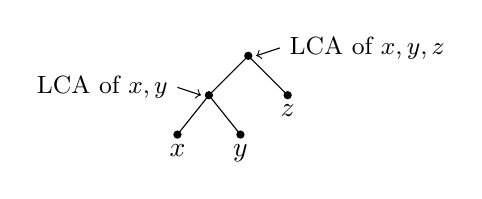
\begin{tikzpicture}
                \coordinate (root) at (0, 0);
                \coordinate (lca) at (-0.5, -0.5);
                \coordinate (z) at (0.5, -0.5);
                \coordinate (x) at (-0.9, -1);
                \coordinate (y) at (-0.1, -1);

                \draw (root) -- (lca);
                \draw (root) -- (z);
                \draw (lca) -- (x);
                \draw (lca) -- (y);

                

                \draw[->] (-0.9, -0.4) node[left] {\small LCA of $x,y$} -- (-0.6, -0.5);
                \draw[->] (0.4, 0.1) node[right] {\small LCA of $x,y,z$} -- (0.1, 0);

                \fill (root) circle (1.5pt);
                \fill (lca) circle (1.5pt);
                \fill (z) circle (1.5pt) node[below] {$z$};
                \fill (x) circle (1.5pt) node[below] {$x$};
                \fill (y) circle (1.5pt) node[below] {$y$};
            \end{tikzpicture}
        }
        & 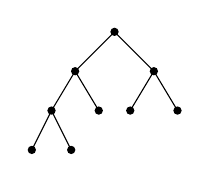
\begin{tikzpicture}
            \coordinate (root) at (0, 0);
            \coordinate (lca1) at (-0.5, -0.5);
            \coordinate (lca2) at (0.5, -0.5);
            \coordinate (lca3) at (-0.8, -1);
            \coordinate (x) at (-0.2, -1);
            \coordinate (y) at (0.2, -1);
            \coordinate (z) at (0.8, -1);
            \coordinate (w) at (-1.05, -1.5);
            \coordinate (v) at (-0.55, -1.5);

            \draw (root) -- (lca1);
            \draw (root) -- (lca2);
            \draw (lca1) -- (lca3);
            \draw (lca1) -- (x);
            \draw (lca2) -- (y);
            \draw (lca2) -- (z);
            \draw (lca3) -- (w);
            \draw (lca3) -- (v);

            \foreach \point in {root, lca1, lca2, lca3, x, y, z, w, v} {
                \fill (\point) circle (1.5pt);
            }
        \end{tikzpicture}
        & 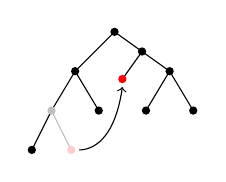
\begin{tikzpicture}
            \coordinate (root) at (0, 0);
            \coordinate (lca1) at (-0.5, -0.5);
            \coordinate (lca2) at (0.7, -0.5);
            \coordinate (lca3) at (-0.8, -1);
            \coordinate (lca3') at (0.35, -0.25);
            \coordinate (x) at (-0.2, -1);
            \coordinate (y) at (0.4, -1);
            \coordinate (z) at (1.0, -1);
            \coordinate (w) at (-1.05, -1.5);
            \coordinate (v) at (-0.55, -1.5);
            \coordinate (v') at (0.1, -0.6);

            \draw (root) -- (lca1);
            \draw (root) -- (lca2);
            \draw (lca1) -- (lca3);
            \draw (lca1) -- (x);
            \draw (lca2) -- (y);
            \draw (lca2) -- (z);
            \draw (lca3) -- (w);
            \draw[gray!50] (lca3) -- (v);
            \draw (lca3') -- (v');

            \foreach \point in {root, lca1, lca2, lca3', x, y, z, w} {
                \fill (\point) circle (1.5pt);
            }

            \fill[gray!50] (lca3) circle (1.5pt);
            \fill[red!20] (v) circle (1.5pt);
            \fill[red] (v') circle (1.5pt);

            \draw[->] (-0.45,-1.5) .. controls (-0.3,-1.5) and (0, -1.4) .. (0.1,-0.7);
        \end{tikzpicture} \\

        \multicolumn{2}{c}{``$x$ is closer to $y$ than $z$''}
        & rooted binary tree
        & relocate a leaf in the tree \\
        \bottomrule
    \end{tabular}
    }
    \caption{An overview of contrastive learning problems studied here (LCA: lowest common ancestor).}
    \label{fig:all-problems}
\end{figure}

Interestingly, even though contrastive information lies at the heart of contrastive learning pipelines, the history of using ordinal information, i.e., comparisons instead of absolute numerical values, dates back to the 1960s in psychometrics and (non-metric) multi-dimensional scaling %because humans tend to be accurate when comparing alternatives, yet terrible when numerically estimating similarities~
\citep{torgerson1952multidimensional,thurstone1954measurement,kruskal1964nonmetric}. %, especially when the goal is to measure human sentiments about political figures, or ranking alternatives.  
Since then, \textit{ordinal} embeddings (also monotone or contrastive embeddings~\citep{bilu2005monotone,chen2022learning,chatziafratis2024dimension}) are widely-studied in computer science, because important applications (nearest-neighbor, recommendation, ranking, crowdsourcing) only care to preserve the relative ordering of distances (not  lengths)~\citep{agarwal2007generalized,buadoiu2008ordinal,tamuz2011adaptively,vankadara2019insights,ghosh2019landmark}.

Despite empirical successes, various aspects of contrastive learning are not well-understood. To address this, works on theoretical foundations have focused on generalization~\citep{alon2023optimal}, inductive bias~\citep{saunshi2022understanding,haochen2022theoretical}, latent classes~\citep{saunshi2019theoretical}, hard negatives~\citep{robinson2020contrastive,kalantidis2020hard,awasthi2022more}, multi-view redundancy~\citep{tosh2021contrastive}, mutual information~\citep{oord2018representation,hjelm2018learning} and more. 

\vspace{-0.2cm}
\paragraph{Optimization of contrastive objectives.} Our paper focuses on \textit{optimization} aspects of contrastive learning with widely-used objectives, both in discrete and continuous settings (\Cref{fig:all-problems}). The input is a set $\mathcal{C}$ of $m$ triplets $\{(\anc_i, \pos_i^+, \neg_{i}^-)\}_{i = 1}^m$ on a dataset $\mathcal{S}$, with non-negative weights $w_i \ge 0$ indicating the importance of each constraint (see~\citep{robinson2020contrastive,kalantidis2020hard} for benefits of ``hard  negatives'' which are difficult to distinguish from anchor points). The task is to find a representation $f(\cdot)$ respecting the given constraints as much as possible by optimizing Objectives~\ref{obj1},~\ref{obj2},~\ref{obj3} below:%, in other words $f(\cdot)$ should satisfy as many (weighted) triplets as possible, or minimize loss from violated triplets.% (this depends on $f(\cdot)$ and each problem’s semantics). 

\begin{enumerate}[leftmargin=*]
    \item\label{obj1} Triplet Maximization in $\mathbb{R}^d$: Many algorithmic works in contrastive embeddings, aim at maximizing the weight of \textit{satisfied} triplets. We say that a triplet $(\anc_i, \pos_i^+, \neg_{i}^-)$ is satisfied by the embedding $f(\cdot)$, if $\lnorm f(x_i)-f(y_i)\rnorm_2 \le \lnorm f(x_i)-f(z_i)\rnorm_2$. Even the case of $d=1$ (line embedding or ranking) is well-motivated and non-trivial~\citep{arora1995polynomial,arora2002new,GHMRC11,fan2020learning}.
    

%The hope of course is that after training is completed and gradient descent has converged, the neural network has learned a representation $f(\cdot)$ that can be later used in many downstream tasks. Currently, there is a variety of contrastive loss objectives set up in a way that incentivize pushing positive pairs $(x_i,y_i)$ close together in embedding space, while keeping negative pairs $(x_i,z_i)$ far apart, thus steering neural networks towards representations that largely respect the given triplets. 

    
    \item \label{obj2} Triplet Maximization on trees: %A mapping of data to the leaves of a tree $T$ is called a hierarchical clustering. 
    Here, we map data onto leaves of a tree $T$ maximizing the weight of satisfied triplets %A triplet $(\anc_i, \pos_i^+, \neg_{i}^-)$ is satisfied if 
    ($\dist_T(x_i,y_i) \le  \dist_T(x_i,z_i)$, or equivalently, $T$ has a subtree containing $\anc_i, y_i$, but not $z_i$). Such hierarchical clustering problems known as triplet reconstruction or consistency naturally appear across areas~\citep{aho1981inferring,byrka2010new,vikram2016interactive,bodirsky2017complexity,chatziafratis2018hierarchical,emamjomeh2018adaptive}.  

    \item \label{obj3} Minimize Triplet Loss in $\mathbb{R}^d$: %\textcolor{red}{we need a convex compact domain, e.g. $[0, 1]^d$} \vnote{we can say it that we restrict to the box in the technical section, but for now R to the d is fine for intro I believe. we can discuss it tomorrow}: 
    The influential FaceNet paper~\citep{schroff2015facenet} introduced the Triplet Loss, which has since evolved into one of the most prominent contrastive losses:
    \begin{align*}
    \mathcal{L}(\mathcal{C},f(\cdot)) \coloneqq \sum_{i=1}^m w_i \mathcal{L}_i, \text{ where } 
    \mathcal{L}_i \coloneqq \max \{\lnorm f(x_i)-f(y_i)\rnorm_2^2 - \lnorm f(x_i)-f(z_i)\rnorm_2^2 + \alpha, 0\}.
    \end{align*}
    %\begin{align*}
    %\mathcal{L}(\{(\anc_i, \pos_i^+, \neg_{i}^-)\}_{i = 1}^m) &\coloneqq \sum_{i=1}^m w_i \mathcal{L}_i, \text{ where } \\
    %\mathcal{L}_i &\coloneqq \max \{\lnorm f(x_i)-f(y_i)\rnorm_2^2 - \lnorm f(x_i)-f(z_i)\rnorm_2^2 + \alpha, 0\}.
    %\end{align*}
    The margin  $\alpha$ specifies the minimum gap of distance $(x_i,y_i)$ and $(x_i,z_i)$ and $w_i$ is the importance of a triplet. This loss ``pushes'' positive pairs close together while keeping negative pairs far apart.
\end{enumerate}

Our primary motivation is to understand the complexity of finding representations based on contrastive information. Unfortunately, $\mathsf{NP}$-hardness results prevent us from finding \textit{globally} optimum representations in the worst-case, and so in practice, local search algorithms are deployed. Local search is a general algorithmic approach that examines improving moves from a set of allowable nearby configurations to the current solution (most notably gradient-based methods and various heuristics in discrete optimization~\citep{orlin2004approximate}). We ask the following basic questions: 
\begin{center}
%\textit{How easy (or hard) is it to find a \emph{locally optimum} representation instead? Will gradient descent or other local search methods converge in polynomial time, or is exponential time sometimes necessary?}
\textbf{Motivating Questions: }\textit{How hard is it to find a \emph{locally optimum} representation for contrastive learning? Can we find a local optimum in polynomial time? How efficient is local search?}
\end{center}

In this context, a locally optimum representation is one that cannot be improved by taking further steps of gradient-based methods, or generally \textit{any} type of local search algorithm.

%Here, we examine common choices of representations $f(\cdot)$, such as (i) $d$-dimensional Euclidean embeddings, (ii) tree embeddings and (iii) line embeddings (1-dimensional Euclidean embeddings). For example, if $f:\mathcal{S}\to \mathbb{R}^d$, we require that the anchor is closer to the positive example than the negative $\lnorm f(x_i)-f(y_i)\rnorm_2 \le \lnorm f(x_i)-f(z_i)\rnorm_2$, whereas if we aim for a tree representation $T$ (also known as hierarchical clustering), we require that $\dist_T(x_i,y_i) \le  \dist_T(x_i,z_i)$, where $\dist_T(\cdot,\cdot)$ denotes the tree distance metric. We note that many well-studied problems in the literature fall under our framework, including the popular Triplet Loss objective~\citep{schroff2015facenet} in the continuous setting, whereas in the discrete setting where we maximize total weight of satisfied triplets, important problems include Triplet Reconstruction in $\mathbb{R}^d$ or with tree metrics, and line embeddings (for $d=1$).




%-In fact, as we will our results are general and can encompass and type of local search algorithm.


%-important of local search in such problems

%This paper is not about the quality of the local optimizers. Convergence...

%In fact, we answer such questions under the unifying framework of local search.

%We do not restrict ourselves to particular methods, such as neural networks with gradient-descent, but rather we focus on general polynomial time algorithms.

%Motivated by the overall lack of guarantees, our work is the first to show and pinpoint a complexity-theoretic reason why even in simple settings.

%how fast does gradient descent local search


%\paragraph{Contrastive Objectives.} In all problems, the input will be a collection of $m$ contrastive triplets $\{(\anc_i, \pos_i^+, \neg_{i}^-)\}_{i = 1}^m$ on the dataset $\mathcal{S}$, weighted by non-negative weights $w_i \ge 0$ indicating the importance of each triplet constraint.



\subsection{Our contributions}



Our main contribution is to formally study the above questions from the lens of computational complexity, and give strong evidence that for many problems with contrastive objectives, even finding a \textit{locally} optimum solution for the objectives is intractable in a specific formal sense. Local search is a widely-used heuristic for many $\mathsf{NP}$-hard problems~\citep{lawler1985traveling,schaffer1991simple,ahuja2002survey,orlin2004approximate}, wherein we iteratively perform local moves (e.g., gradient step or reassignment of points) that get better objective value, terminating at a solution with no improving move, i.e., a \textit{local} optimum.  Of course, a local optimum need not be a global optimum, and since there are more local optima than global optima in general, local optima  may appear  easier to find.  Nevertheless, there is currently an overall lack of theoretical guarantees regarding local optimization of the contrastive objectives~\ref{obj1},~\ref{obj2},~\ref{obj3}; indeed, it is not even clear whether there is a polynomial-time algorithm for computing a local optimum. Our main result is to show that no such polynomial time algorithm exists (unless there is an unlikely collapse of complexity classes, see below). Moreover, an unconditional consequence of our reductions, is that there exist contrastive learning instances where local search algorithms (including gradient-based methods) require \textit{exponential} time before reaching a local optimum. To the best of our knowledge, we are the first to formally investigate the complexity of local solutions in contrastive learning objectives.%, and establish formal connections with the complexity of local search.





%Could it be that no efficient algorithm for the latter problem exists? If so, how can we prove it? If we can’t prove it, how can we nevertheless amass evidence of intractability? These questions are, of course, addressed by the theory of NP-completeness. This lecture and the next describe analogs of NP-completeness for equilibrium computation problems.

%We are not the first to study locally optimal solutions in complexity. Indeed, complexity theory focused on this. NP-hardness gave us a beautiful theory for hard to solve problems in terms of computing globally optimal solutions. The analog here is PLS for discrete problems MAX CUT, circuit FLIP etc.  CHALLENGE: pls reductions preserving local optima





\vspace{-0.2cm}
\paragraph{Proving hardness of local optima.} The remarkable theory of $\NP$-hardness was developed to understand the difficulty of computing the value of a \textit{global} optimum in optimization problems. Hence, $\NP$-hardness is not suitable to describe local optimality, which corresponds to fixed points of local search algorithms. \citet*{johnson1988easy} initiated the complexity-theoretic study of discrete local search problems by defining the complexity class $\mathsf{PLS}$ ($\mathsf{P}$olynomial $\mathsf{L}$ocal $\mathsf{S}$earch), and later,~\citet{daskalakis2011continuous} defined the class $\mathsf{CLS}$ ($\mathsf{C}$ontinuous $\mathsf{L}$ocal $\mathsf{S}$earch) for continuous local search problems. Due to the significance of computing fixed points, both $\mathsf{PLS}$ and $\mathsf{CLS}$ have played a prominent role in optimization and algorithmic game theory. For example, computing a pure Nash equilibrium in congestion games is $\PLS$-hard~\citep{fabrikant2004complexity}, and it was recently shown that computing a Karush-Kuhn-Tucker point (fixed points of gradient-descent) of a quadratic program is $\CLS$-hard~\citep{fearnley2024complexity}. Surprisingly, even though $\mathsf{PLS}$ and $\mathsf{CLS}$ were originally defined with very different problems in mind, a recent breakthrough~\citep*{Fearnley23:Complexity} established a deep connection between them,\footnote{$\mathsf{PPAD}$ captures computation of mixed Nash equilibria, see celebrated work of~\cite{daskalakis2009complexity}.} i.e., that $\mathsf{CLS}=\mathsf{PLS}\cap\mathsf{PPAD}$. Building on it, \citet{Babichenko21:Settling,Anagnostides23:Algorithms,
ghosh2024complexitysymmetricbimatrixgames, anagnostides2025complexitysymmetricequilibriaminmax} have shown  that broad classes of games, including congestion games and adversarial team games, are captured by $\CLS$. Beyond games, for connections of $\mathsf{PLS}$ and $\mathsf{CLS}$ to cryptography, see~\citet{bitansky2020cryptographic,hubacek2020hardness}. Our work provides formal evidence of computational intractability of finding local optima in contrastive learning:



\begin{theorem*}[Abridged; see Theorems~\ref{thm:local-contrastive-dd},~\ref{thm:local-betweenness-dd},~\ref{thm:local-contrastive-tree},~\ref{thm:CLS_hard_contrastive}]
Triplet maximization problems~\ref{obj1},~\ref{obj2} are $\PLS$-hard, i.e., every problem in $\PLS$ efficiently reduces to them. The Triplet Loss minimization problem~\ref{obj3} is $\CLS$-hard, i.e., every problem in $\CLS$ efficiently reduces to it. As a corollary, assuming the widely-believed $\mathsf{PLS}\nsubseteq\mathsf{P}$ and $\mathsf{CLS}\nsubseteq \mathsf{P}$, no polynomial time algorithm (local search or otherwise) can find a \textit{local optimum} of  objectives \ref{obj1}, \ref{obj2}, \ref{obj3}. Even if $\mathsf{PLS}\subseteq\mathsf{P}$ or $\mathsf{CLS}\subseteq \mathsf{P}$, there exist instances where local search (including gradient-methods) require exponential time to reach a local optimum. 
\end{theorem*}
   
\vspace{-0.1cm} 
Formal statements are in Section~\ref{sec:hardness-pls},~\ref{sec:hardness-cls}. %, after defining the input/output of the local versions for the contrastive objectives \ref{obj1}, \ref{obj2}, \ref{obj3}. 
As is common in complexity, polynomial time refers to algorithms whose runtime is polynomial in the input size (provided in binary representation). Our results also extend to \textit{approximate} local optima (solutions within a small $\epsilon>0$ from a local optimum).

\vspace{-0.1cm}
\paragraph{Challenges and proof ideas.} The consequence of proving that a problem is $\mathsf{PLS}$-hard (or $\mathsf{CLS}$-hard) is that in a certain precise sense, such problems are as hard as any other local search problem where the goal is to find a local optimum. Here, local optimality is defined  with respect to a generic definition of a local search algorithm~\citep{johnson1988easy,daskalakis2011continuous}. The main technical challenge in all works establishing hardness results is how to do $\mathsf{PLS}$-reductions (or $\mathsf{CLS}$-reductions). Roughly speaking, these are special type of efficient transformations between problems, that preserve \textit{local} optimality: the intuition is that starting from an already-known hard problem, and using a $\mathsf{PLS}$-reduction to another problem, e.g., the contrastive objectives above, then any efficient algorithm that purportedly finds a local optimum of the latter, would in fact compute a local optimum of the original (known-to-be-hard) problem. Contrast this with the common $\mathsf{NP}$-reductions that are only required to preserve the value of global optima, ignoring how local solutions are being altered. 

Our results provide $\mathsf{PLS}$-reductions from the \textsc{LocalMaxCut} problem~\citep{schaffer1991simple} (see~\Cref{sec:prelim} for definitions) to the maximization of satisfied triplets (Obj.~\ref{obj1},~\ref{obj2}), and a $\mathsf{CLS}$-reduction from \textsc{QuadraticProgram-KKT}~\citep{fearnley2024complexity} to the Triplet Loss (Obj.~\ref{obj3}). Our $\PLS$-reductions rely on novel gadgets that allow us to encode graph cuts and local (vertex) moves via triplet constraints and embeddings in Euclidean space, trees or even the line (for the case of rankings).  Our gadgets impose a series of ``heavy'' contrastive triplet constraints on a special set of ``boundary'' points, thus ensuring they are not allowed to move back and forth, otherwise the objective value would drift away from any local optimum. After an embedding is performed, the two sides of the graph cut can be formed by looking at which nodes were placed to the ``left'' or ``right'' of the boundary points. Regarding our $\CLS$-reductions, we encode and recover KKT stationary points of quadratic programs $\min_{\vx \in [0, 1]^n} \vx^\top \mat{Q} \vx + \vb^\top \vx$, by finding local minima of Triplet Loss, even if the representation $f(\cdot)$ comes from a simple linear embedding model parameterized by $\vtheta \in [0, 1]^n$ such that $f_{\vtheta}(\vx) = \vtheta^\top \vx$. Towards this, we first break the quadratic form into triples of variables $x, y, z \in [0, 1]$ and we generate a specially crafted collection $\mathcal{T}$ of contrastive triplets $(x_i,x_j^+,x_k^-)$, where $x_i,x_j,x_k$ are coordinates of $\vx$. However, contrastive constraints introduce dependencies among their shared variables and to deal with the interacting terms, we introduce groups of contrastive triplets with carefully chosen weights that depend on the coefficients of the quadratic form.

%In our case, we provide $\mathsf{PLS}$-reductions from the \textsc{LocalMaxCut} problem~\citep{schaffer1991simple} to the maximization of satisfied triplets over $\mathbb{R}^d$ or trees (objectives~\ref{obj1},~\ref{obj2}, and few other related objectives), and a $\mathsf{CLS}$-reduction from \textsc{QuadraticProgram-KKT}~\citep{fearnley2024complexity} to the Triplet Loss (objective~\ref{obj3}). To give some intuition to the reader about our $\PLS$-reductions, starting from a graph max cut instance, we build novel gadgets that allow us to encode graph cuts and local (vertex) swaps to different sides, via the use of triplet constraints and embeddings of the points in euclidean space or tree metrics or even the line (for the case of rankings). To encode the notion of a graph cut, i.e., that points need to be split in two sides $(S,\bar{S})$, our gadgets impose a series of ``heavy'' contrastive triplet constraints on a special set of nodes $R$ (think of them as ``boundary'' points), thus ensuring that they are not allowed to move back and forth, otherwise the contrastive objective value would drift away from any local optimum. The rest of the constraints are ``edge'' constraints indicating how the rest of the nodes must be placed with respect to the boundary points. After an embedding is performed, due to the edge constraints, we can measure in some sense the value of the cut: the two sides of the graph cut $(S,\bar{S})$ can be formed by looking at which nodes were placed to the ``left'' or ``right'' of the boundary points $R$. In reality, there is no left or right side for the underlying metric space, but based on the distances of points after the embedding, we can still recover a graph cut in a natural way. Importantly, our analyses show that local optima found after the embedding are indeed local optima for the original max cut instance thus concluding the steps needed in a $\PLS$-reduction. 

%\vnote{5 line summary of below. put in each section.}

%Regarding our $\CLS$-reductions, we show how to encode and recover KKT stationary points in quadratic programs of the form $\min_{\vx \in [0, 1]^n} \vx^\top \mat{Q} \vx + \vb^\top \vx$, by finding local minima of Triplet Loss on a specially crafted collection $\mathcal{T}$ of contrastive triplets $(x_i,x_j^+,x_k^-)$ on coordinates of $\vx$, whose individual contribution to the loss is $\mathcal{L}_{ijk} \coloneqq \max \{\lnorm f(x_i)-f(x_j)\rnorm_2^2 - \lnorm f(x_i)-f(x_k)\rnorm_2^2 + \alpha, 0\}$. In fact, our reductions work even if the representation $f(\cdot)$ comes from a simple linear embedding model  parameterized by $\vtheta \in [0, 1]^n$ such that $f_{\theta}(\vx) = \vtheta^\top \vx$. To simplify exposition here, let us focus on the 1-dimensional case (see problem \Contrastive) where each point gets assigned to a number in $[0,1]$. A local solution $\bm{a}^* = (a_0^*, a_1^*, \dots, a_n^*) \in [0, 1]^n$ is said to be a local minimum of \Contrastive, if for any $i \in [1, n]$ and any other local move $a_i \in [0, 1]$, the following variational inequality holds $    \langle a_i - a^*_i, \nabla_{a_i} \mathcal{L}(\va^*)\rangle \geq 0$, where $\mathcal{L}(\va^*)=\sum_{\mathcal{T}} w_{ijk}\mathcal{L}_{ijk}$. The main obstacle is how to encode an arbitrary quadratic function of $n$ variables. We achieve this by first breaking the quadratic form into triples of variables $x, y, z \in [0, 1]$: $q(x, y, z) \coloneqq c_1 x^2 + c_2 y^2 + c_3 z^2 + c_4 xy + c_5 xz + c_6 yz + c_7 x + c_8 y + c_9 z$. Unfortunately, because contrastive constraints involve 3 variables at a time, this introduces correlation/dependencies among the different triplets since there are shared variables. To overcome the difficulty of the interacting terms, we introduce 12 contrastive triplets (and their \textit{dual} constraints) on $x,y,z$, whose corresponding weights depend on the coefficients of the given quadratic. By solving a linear system for the weights, we manage to obtain that $\mathcal{L}_{xyz}$ is the same as $q(x, y, z)$. Summing those recovers $\vx^\top \mat{Q} \vx + \vb^\top \vx$. 




%\vnote{should i mention here that x squared cancels out and so our gadgets introduce several constraints to encode the quadratic? how to motivate the reference points 0 and 1/2? or maybe just ignore them?}

 



%-we are first to study local complexity and theoretically prove the hardness
%which transform a known difficult problem to the task at hand, in a way that preserves local optimality. Our main techniques involve the so-called $\mathsf{PLS}$-reductions and $\mathsf{CLS}$-reductions, which are special types of reductions that preserve local optimality between solutions of problems (in particular, they differ significantly from standard $\mathsf{NP}$ reductions). For example, a direct consequence of our results is that finding local optima for the Triplet Loss objective~\citep{schroff2015facenet} may require exponentially many iterations no matter what gradient-based method is being used, even for linear models. Similarly, for embedding points in $d$-dimensional Euclidean space or onto a tree metric subject to a given collection of contrastive triplets, any local search algorithm requires exponential time in the worst-case. 

%While it is still unknown whether PLS is in P, it is widely believed that PLS not equal to P.

%Our main results here is to prove PLS and CLS hardness for problems in contrastive learning:




%By now, there are several works 
%with a growing-list of broad class of game dynamics have been shown to be captured by $\CLS$ \citep{fearnley2024complexity,Anagnostides23:Algorithms,ghosh2024complexitysymmetricbimatrixgames, Hollender24:Complexity, anagnostides2025complexitysymmetricequilibriaminmax}.
%\textcolor{red}{For example, it is well-known that computing a pure Nash equilibrium of congestion games is $\PLS$-hard but the complexity of finding a (possibly mixed) Nash equilibrium remained elusive for a long time. It was until recent breakthrough where \cite{Fearnley23:Complexity} proved that $\CLS = \PPAD \cap \PLS$ and building on their work, \cite{Babichenko21:Settling} showed that is $\CLS$-complete to find a Nash equilibrium in congestion games. More recently, the complexity of finding Karush-Kuhn-Tucker (KKT) point of a quadratic program, along with the complexity of finding Nash equilibria in a broad class of games, have been shown to be captured by $\CLS$ \citep{fearnley2024complexity,}


%computing a KKT point of a quadratic polynomial over the domain [0, 1]n is complete for the class CLS = PPAD ∩ PLS

%Our goal is to prove that the problem of computing a local optimum of a maximum cut instance is as hard as any other local search problem. Having formalized “any other search problem,” we now formalize the phrase “as hard as.” This done using reductions, which are familiar from the theory of NP-completeness. Formally, a reduction from a problem L1 ∈ P LS to a problem L2 ∈ P LS is two polynomial-time algorithms: 1. Algorithm A maps every instance x ∈ L1 to an instance A(x) ∈ L2. 2. Algorithm B maps every local optimum of A(x) to a local optimum of x. The definition of a reduction ensures that if we can solve the problem L2 in polynomial time then, by combining it with algorithms A and B in the reduction in the natural way, we can also solve the problem L1 in polynomial time. Definition 2.1 ([2]) A problem L ∈ P LS is PLS-complete if every problem of P LS reduces to it. By definition, there is no polynomial-time algorithm for computing a local optimum of a P LS-complete problem, unless P LS ⊆ P . Most researchers believe that P LS 6 ⊆ P , though confidence is not as strong as for the P 6 = N P conjecture. A

%and have intricate connections to other celebrated classes such as PPAD (check recent breakthrough best paper)

%such as game theory,  

%leading to recent breakthroughs for fixed point computations fixed point of gradient descent and connections between them PPAD celebrated work STOC 2022 best paper, results proving congestion games being PLS hard, KKT CLS hard

%We study search problems that can be solved by performing Gradient Descent on a bounded convex polytopal domain and show that this class is equal to the intersection of two well-known classes: PPAD and PLS. As our main underlying technical contribution, we show that computing a Karush-Kuhn-Tucker (KKT) point of a continuously differentiable function over the domain [0,1]2 is PPAD ∩ PLS-complete. This is the first non-artificial problem to be shown complete for this class. Our results also imply that the class CLS (Continuous Local Search) - which was defined by Daskalakis and Papadimitriou as a more "natural" counterpart to PPAD ∩ PLS and contains many interesting problems - is itself equal to PPAD ∩ PLS.

%we are the first to do so...tools ideas from complexity to study contrastive learning, conceptual contribution of our work...ordinal embeddings, and contrastive learning very new setting...





%Generally, we show an unconditional result for the runtime of local search algorithms(broadly defined, see Preliminaries) for contrastive learning, proving that converging to local optima needs exponential time. Furthermore, unless there is a surprising collapse for the aforementioned complexity classes, i.e., that $\mathsf{PLS}\subseteq \mathsf{P}$ or $\mathsf{CLS}\subseteq \mathsf{P}$, no polynomial time algorithm (local search or otherwise) can find a local optimum for the problems that we consider in this paper. 

% \jy{I am not sure if we should move the above paragraph into the experimental section, I understand the reason it appears here and it seems a bit repetitive with the next paragraph.}



% \textcolor{red}{We want to note that this is the first work considering the computational complexity of finding local solutions for contrastive learning.}
%Before stating our results, we describe here the different categories of problems considered in this paper, depending on what objective we are optimizing and what type of representation we are seeking. 

%\vnote{i agree currently there is a bit of repetition. but i am not done with intro. Please edit after I am done otherwise things get confusing.}




%recent breakthrough

% For example, consider the special case of maximum cut instances in which every edge has unit weight. Computing a global maximum remains an NP-hard problem, but computing a local maximum is easy. Because the objective function in this case can only take on the values {0, 1, 2, . . . , |E|}, local search terminates (at a local maximum) in at most |E| iterations. 

%How might we amass evidence that no such algorithm exists? The strongest type of negative result would be an unconditional one: a proof that there is no polynomial-time algorithm for the problem. No one knows how to prove unconditional results like this; in particular, such a result would separate P from N P . Instead, a natural response is to try to prove that finding local maxima of maximum cut instances is an NPcomplete problem. In the next lecture we’ll see why this is also too strong a negative result to shoot for. Instead, we’ll develop an analog of NP-completeness tailored for local search problems.

%Our goal is to prove that the problem of computing a local optimum of a maximum cut instance is as hard as any other local search problem. Having formalized “any other search problem,” we now formalize the phrase “as hard as.” This done using reductions, which are familiar from the theory of NP-completeness. Formally, a reduction from a problem L1 ∈ P LS to a problem L2 ∈ P LS is two polynomial-time algorithms: 1. Algorithm A maps every instance x ∈ L1 to an instance A(x) ∈ L2. 2. Algorithm B maps every local optimum of A(x) to a local optimum of x. The definition of a reduction ensures that if we can solve the problem L2 in polynomial time then, by combining it with algorithms A and B in the reduction in the natural way, we can also solve the problem L1 in polynomial time.

%Johnson et al. [2] proved that a problem concerning Boolean circuits called “CircuitFlip” is PLS-complete. Once a first complete problem is identified, more can be obtained via reductions. Some such reductions were given in [2] and many more, including to the maximum cut problem, were given in [3]

%This parallels the idea that for NP-complete problems, we don’t expect there to be an algorithm that improves significantly over brute-force search. A byproduct of the theory developed in this and the next section is exponential lower bounds on the number of iterations required by local search to reach a local optimum.




%\jy{We have formally define the problem in the other overleaf file, consider copy them will and add more detials.}
%\vnote{thanks i will.}








%\subsection{Other Related Work}

%must link cannot link constraints, here is the analog but for 3 points at a time...and we want to do representation learning...explain motivation for discrete problems, pls cls importance


\section{Preliminaries}\label{sec:prelim}
%Here, we provide the necessary background on $\PLS, \CLS$ to understand our complexity results, and we define the contrastive learning objectives (discrete and continuous) for which we prove  hardness.

\subsection{Discrete objectives in contrastive learning and \texorpdfstring{$\PLS$}{PLS}}

\citet{johnson1988easy} defined $\PLS$ to describe local search problems. A problem $\Pi$ is in $\PLS$ if the following three polynomial-time algorithms exist:~\footnote{Both $\PLS$ and $\CLS$ can be equivalently defined with arithmetic circuits~\citep{Fearnley23:Complexity}} (i) the first algorithm, given an instance of $\Pi$, it outputs an arbitrary feasible solution $S$, (ii) the second, given $S$, it returns a number which is the objective value of the feasible solution, and (iii) the third, given $S$, it either reports ``locally optimal'' or produces a better solution. Implicit in the definition is the fact that feasible solutions have polynomially many \textit{neighboring} solutions (the third algorithm is polynomial-time). In this sense, one can think of $\PLS$ as problems with efficient verification of \textit{local} optimality.


\begin{definition}[$\PLS$-reduction]
A $\PLS$-reduction from problem $\Pi_1$ to problem $\Pi_2$ is two polynomial-time algorithms: (i) the first algorithm $A$ maps every instance $x$ of $\Pi_1$ to an instance $A(x)$ of $\Pi_2$, and (ii) the second algorithm $B$ maps every local optimum of $A(x)$ to a local optimum of $x$.
\end{definition}
A $\PLS$-reduction ensures that if we find a local optimum for $\Pi_2$ in polynomial time then, we could also find a local optimum for $\Pi_1$ in polynomial time. A problem is $\PLS$-hard if every problem in $\PLS$ can be reduced to it. In complexity, it is widely-believed that $\PLS\nsubseteq \P$, hence there is no polynomial-time algorithm for computing a local optimum of a $\PLS$-hard problem. Interestingly,~\citet{schaffer1991simple} proved many natural problems are $\PLS$-hard, including \textsc{LocalMaxCut}:

\begin{nproblem}[\textsc{LocalMaxCut}]\label{def:maxcut}
 \textsc{Input :} A weighted undirected graph $G(V,E)$ with a non-negative weight $w_{e}\ge0$ for each edge.
\\
  \noindent \textsc{Output :}  A partition $(S,\bar{S})$ of the vertices $V$ in two nonempty sets, such that no vertex $v$ can increase the value of the cut, i.e., the sum of weighted edges cut, by switching sides.
\end{nproblem}

We now define widely-used (discrete) objectives of maximizing satisfied contrastive constraints. To simplify notation, from now on we drop the signs and simply write $(\anc_i, \pos_i, \neg_{i})$ for contrastive triplets. All embeddings here  map a set of $n$ items to non-overlapping points of a metric space.%In all cases the input is a set $V$ of $n$ vertices, together with a set of $m$ contrastive triplets $\{(\anc_i, \pos_i^+, \neg_{i}^-)\}_{i = 1}^m$ where $x_i,y_i,z_i\in V$. Each triplet has a non-negative weight $w_i \ge 0$.


\begin{nproblem}[\textsc{LocalContrastive-Euclidean}] \label{def:local-euclidean}
\textsc{Input :} Set $V$ of $n$ vertices, together with $m$ contrastive triplets $\{(\anc_i, \pos_i, \neg_{i})\}_{i = 1}^m$ where $x_i,y_i,z_i\in V$ (we dropped the $+/-$ signs for lighter notation). Each triplet has a non-negative weight $w_i \ge 0$.
\\
  \noindent \textsc{Output :}  An embedding $f: V \to \mathbb{R}^d$ such that no vertex $v$ can increase the value of the embedding by switching its location in $\mathbb{R}^d$. We say a constraint $(x_i, y_i, z_i)$ is \emph{satisfied} by $f(\cdot)$, if $x_i$ is placed closer to $y_i$ than to $z_i$, i.e.,  $\|f(x_i) - f(y_i)\|_2 \leq \|f(x_i) - f(z_i)\|_2$. The embedding's objective value is $\sum_{i=1}^m w_i \cdot \mathbf{1}_{(x_i, y_i, z_i)}$, where $\mathbf{1}_{(x_i, y_i, z_i)} = 1$ if the constraint is satisfied by $f(\cdot)$, and 0 otherwise.
\end{nproblem}

%In the following two problems, the input is exactly the same, but the type of embedding and consequently what it means to satisfy a triplet $(\anc_i, \pos_i, \neg_{i})$ may be changed accordingly:

\begin{nproblem}[\textsc{LocalContrastive-Tree}] \label{def:local-tree}
\textsc{Input :}  As above, set $V$  with contrastive triplets $\{(\anc_i, \pos_i, \neg_{i})\}_{i = 1}^m$ (non-negative weights $w_i \ge 0$).
\\
  \noindent \textsc{Output :}  A hierarchical clustering, i.e., a binary rooted tree $T$ with $|V|$ leaves, and a 1-to-1 mapping from $V$ to the leaves of $T$, such that no vertex $v$ can increase the value of the tree by switching to another location in the tree $T$ (for each $v$ in $T$, there are exactly $2|V|-3$ other candidate locations). We say a triplet $(x_i, y_i, z_i)$ is \emph{satisfied} by $T$, if $x_i$ is placed closer to $y_i$ than to $z_i$, i.e., if there is a subtree in $T$ containing $x_i,y_i$ but not $z_i$ (this is equivalent to $\dist_T(x_i,y_i)\le\dist_T(x_i,z_i)$ for an ultrametric distance on $T$). The tree's objective value is $\sum_{i=1}^m w_i \cdot \mathbf{1}_{(x_i, y_i, z_i)}$.
\end{nproblem}

Moreover, we examine scenarios where provided contrastive information is of the form ``among $x,y,z$, items $x,z$ are \textit{farthest} apart'' (instead of indicating that ``item $x$ is closer to $y$ than to $z$''). Already for 1-dimensional embeddings, such constraints give rise to \textsc{Betweenness}, a well-studied ranking problem in approximation algorithms~\citep{arora2002new,charikar2009every,austrin2015np}.

\begin{nproblem}[\textsc{LocalBetweenness-Euclidean}] \label{def:local-ranking}
\textsc{Input :} Set $V$  with \textit{betweenness} triplets $\{(\anc_i, \pos_i, \neg_{i})\}_{i = 1}^m$ each with a non-negative weight $w_i \ge 0$.
\\
  \noindent \textsc{Output :}  An embedding $f: V \to \mathbb{R}^d$ such that no vertex $v$ can increase the value of the embedding by switching its location in $\mathbb{R}^d$. We say a constraint $(x_i, y_i, z_i)$ is \emph{satisfied} by $f(\cdot)$, if $x_i$ and $z_i$ are placed the farthest apart (equivalently, $y_i$ is ``between'' $x_i$ and $z_i$), i.e., $\|f(x_i) - f(z_i)\|_2 \ge \max\{\|f(x_i) - f(y_i)\|_2, \|f(z_i) - f(y_i)\|_2\}$. The embedding's objective value is $\sum_{i=1}^m w_i \cdot \mathbf{1}_{(x_i, y_i, z_i)}$.
\end{nproblem}

Even though we defined problems in their general form, our $\PLS$-hardness results also hold for interesting special cases: we show \textsc{LocalContrastive-Euclidean} in dimension $d=1$~\citep{buadoiu2008ordinal,alon2008ordinal,fan2020learning} and \textsc{LocalBetweenness-Euclidean} with $d=1$~\citep{arora2002new,charikar2009every,austrin2015np} are $\PLS$-hard. For trees, \textsc{LocalContrastive-Tree} is also known as triplet reconstruction/consistency~\citep{byrka2010new,chatziafratis2023triplet}. For other extensions, see~\Cref{app:extensions}.


\subsection{Continuous objectives in contrastive learning and \texorpdfstring{$\CLS$}{CLS}}
\citet{daskalakis2011continuous} proposed $\CLS$ to study local search for continuous objective functions, most notably search problems that can be solved by performing Gradient Descent. $\CLS$ has played an important role in game theory and optimization, and a recent breakthrough showed that $\CLS = \PPAD \cap \PLS$ \citep{Fearnley23:Complexity}. The natural problem of finding KKT points in quadratic programs was recently shown to be $\CLS$-hard~\citep{fearnley2024complexity} and we will reduce it to finding local minima of the Triplet Loss~\citep{schroff2015facenet}. 


%$\CLS$ was proposed to serve as a complexity framework for understanding the complexity of problems lying in the intersection of $\PPAD$ and $\PLS$. A recent breakthrough result shows that $\CLS = \PPAD \cap \PLS$ \citep{fearnley2024complexity}. The $\CLS$ complexity class has been instrumental in capturing various problems in optimization and game theory. Notably, the task of finding a Karush-Kuhn-Tucker (KKT) point in quadratic programs has been proven to be $\CLS$-complete \citep{fearnley2024complexity}.



\begin{nproblem}[\textsc{QuadraticProgram-KKT}] \label{def:quadratic}
\textsc{Input :} A symmetric matrix $\mat{Q} \in \mathbb{R}^{n \times n}$ and vector $b\in \mathbb{R}^{n}$.
\\
  \noindent \textsc{Output :} Compute a local optimum (i.e., a KKT point) for the quadratic $\min_{\vx \in [0, 1]^n} \vx^\top \mat{Q} \vx + \vb^\top \vx$.
    
\end{nproblem} 



\begin{nproblem}[\textsc{LocalTripletLoss-Euclidean}] \label{def:local-loss}
\textsc{Input :} Set $V\cup\{A,B\}$ of points in $\mathbb{R}^d$, set $\cal{C}$ of triplets $(\vx, \vy, \vz)$ of weight $w \ge 0$, margin $\alpha>0$.
\\
  \noindent \textsc{Output :}  Find an embedding $f: V \to [0,1]^d$ that is a first-order stationary point for the minimization objective given by the triplet-loss:\[\sum_{(\vx, \vy, \vz)\in \cal{C}} w \cdot \max \left\{\norm{f(\vx) - f(\vy)}_2^2 - \norm{f(\vx) - f(\vz)}_2^2 + \alpha, 0\right\}.\] 
\end{nproblem}

Recall, first-order stationary points are fixed points of gradient descent: $\vx^* \in \calX$ is a first-order stationary point of $g(\vx)$, if $\forall \vx \in \cal{X}$ we have $\langle\vx - \vx^*, \nabla_{\vx} g(\vx^*)\rangle \geq 0$ ($\cal{X}$: convex, compact domain). 

We emphasize the role of the two pivot points $A,B$ in the definition. Notice that if we did not have pivot points, then the embedding that maps all points from $V$ to the all-zeros vector would be a trivial first-order stationary point. Moreover, if we had only 1 pivot $A$, then again mapping every point in $V$ to $A$ would result in a first-order stationary point of the Triplet Loss. Thus having two pivot points are necessary and sufficient to make the problem non-trivial.


%\vnote{done with prelims but may polish later, i go edit sec 3 now}


%We emphasize that even for 
%Here, we focus on KKT points for the Triplet Loss~\citep{schroff2015facenet}:

%-observe previous objectives have discrete objective in that a solution either satisfied a constraitns or violated it. but what if the loss is real number? then Daskalakis papadimitriou defined CLS etc....

%\vnote{almost done here, finishing up the continuous case, then going to Sec 3.}




%(also called \textsc{MaxCut/Flip})
%We first introduce the notations we use throughout this paper. \cref{sec:prelim_objective} reviews the contrastive learning problems and the corresponding objectives we study. In \cref{sec:prelim_complexity} we present definitions of local search and relevant complexity classes.

%\vnote{interchangeably points, elements, nodes, leaves, variables, vertices depending on the context}

%\vnote{plus minus in achnors don't be confused}
%\paragraph{Notation} We use boldface lowercase letter $\va, \vb, \vc$ to denote vectors and boldface uppercase letter $\mat{A}, \mat{B}$ to denote matrices. For vector norms, $\|\cdot\|_1, \|\cdot\|_2, \|\cdot\|_{\infty}$ denote $\ell_1, \ell_2,$ and $\ell_{\infty}$ norms respectively. \vnote{other than ell 2 do we use any other norm in the paper?} \jy{Not by me}Unless specified otherwise, we use $\|\cdot\|$ to denote the $\ell_2$ norm. For a vector $\vx \in \mathbb{R}^n,$ we let $x_i$ to be the $i^{th}$ coordinate of vector $\vx$. We use $\ve_i$ to denote the $i^{th}$ unit vector and $\bm{1}$ to denote the all-ones vector. Sometimes we use standard asymptotic notations $O(\cdot), \Theta(\cdot), \Omega(\cdot)$ to suppress absolute constants.

%\yl{I sometimes use the same notation for both variables and its embedding for simplicity}

%\subsection{Contrastive Learning Objectives}\label{sec:prelim_objective}

%\jy{Formally argue the difference between discrete and continuous case}
%In this section, we define the problems for which we will prove that finding local solutions is computationally intractable. 

% We consider a general class of contrastive learning problems defined over a ground set $V$ and a collection of weighted constraints
% \[
% \mathcal{C} = \{(t_i, w_i)\}_{i=1}^m, \quad \text{where } t_i = (v_i^1, \dots, v_i^k) \in V^k \text{ with all } v_i^j \text{ distinct, and } w_i > 0.
% \]
% A \emph{solution} is an injective embedding $f: V \to \mathcal{X}$ into a metric space $(\mathcal{X}, \dist)$ such that $f(u) \neq f(v)$ for all $u \neq v$. Each constraint $(t_i, w_i)$ is associated with a predicate $P_{t_i}$, and is said to be \emph{satisfied} if $P_{t_i}(f)$ evaluates to true.

% The goal is to maximize the total weight of satisfied constraints:
% \[
% \score(f) = \sum_{i=1}^m w_i \cdot P_{t_i}(f),
% \]
% A \emph{local move} modifies the embedding by changing the location of a single element $v \in V$, while maintaining $f(u) \neq f(v)$ for all $u \neq v$. A solution $f$ is a \emph{local optimum} if no such move improves the score.

% We study several concrete instantiations of this framework... 

%\yl{I plan to create a table (similar to Figure 1 in \url{https://arxiv.org/pdf/2102.11548}) for the problems we study.}



%We study several discrete contrastive learning objectives, each defined over a set $\calS$ of $n$ elements and a collection of $m$ weighted constraints of the form $t_i = (x_i, y_i^{+}, z_i^{-})$ on the set $\calS$ with positive weight $w_i$. Each constraint is satisfied if a predicate on $t_i$ holds in the given representation. The goal is to find a \textcolor{red}{local} solution that maximizes the total weight of satisfied constraints. We define a local move as a modification to the current solution that only affects a single element in $V$, and say a solution is a local optimum if no such move increases the score.

% \paragraph{Ranking on the line with triplet constraints. } We define two problems in which the main task is given $n$ objects and a set of $m$ triplet constraints, output an ordering on the line that maximizes the total weight of satisfied constraints.
\iffalse
\subsubsection{Embedding on a line.}

\begin{definition}[\textsc{Betweenness} Problem]
\end{definition}
\begin{nproblem}[\betweeness] \label{def:betweenness}
 \textsc{Input :}  \begin{itemize}
   \vspace{-0.1in}
   \item A collection $\calS = \{a_1,...,a_n\} $ of $n$ points.
   \item A collection of $m$ triples $t_1,...,t_m$ with positive weights $w_1,...,w_m$. Each triplet $t_i$ is of the form $(x_i,y_i, z_i)$ where $x_i, y_i, z_i$ are different points from set $\calS$. Triplet $t_i$ is satisfied as long as $y_i$ is positioned between $x_i$ and $z_i.$ 
\end{itemize}
  \vspace{-0.1in}
  \noindent \textsc{Output :} \begin{itemize}[label = ]
      \vspace{-0.1in}
      \item A permutation $p^* = (a_1^*, a_2^*, \dots, a_n^*)$ over $\calS$ such that no point can unilaterally change their location in $p^*$ and increase the total weight of the satisfying triplets. 
  \end{itemize}
\end{nproblem}

\begin{definition}[\textsc{Non-Betweenness} Problem]
\end{definition}

\begin{nproblem}[\nbtw]
    \textsc{Input :}  \begin{itemize}
    \vspace{-0.1in}
   \item A collection $\calS = \{a_1,...,a_n\} $ of $n$ points.
   \item A collection of $m$ triples $t_1,...,t_m$ with positive weights $w_1,...,w_m$. Each triplet $t_i$ is of the form $(x_i,y_i, z_i)$ where $x_i, y_i, z_i$ are different points from set $\calS$. Triplet $t_i$ is satisfied if $y_i$ is \textbf{not} positioned between $x_i$ and $z_i.$ 
\end{itemize}
    \vspace{-0.1in}
  \noindent \textsc{Output :} \begin{itemize}[label = ]
      \vspace{-0.1in}
      \item A permutation $p^* = (a_1^*, a_2^*, \dots, a_n^*)$ such that no point can unilaterally change their location in $p^*$ and increase the total weight of the satisfying triplets. 
      \end{itemize}
\end{nproblem}

\yl{Do non-btw if time allows}

Before we proceed to introduce contrastive learning problem when the objective function is continuous, we first present the definition of Karush-Kuhn-Tucker (KKT) point as it will serve as the notion of local solution in the continuous setting.

\begin{definition}[Karush-Kuhn-Tucker (KKT) point]
    Given an optimization problem of the form
    \begin{align*}
        \min_{\vx \in \calX} f(\vx).
    \end{align*}
    We say a point $\vx^* \in \calX$ is a Karush-Kuhn-Tucker (KKT) point if for all $\vx \in \calX$, it holds that
    \begin{align*}
        \langle\vx - \vx^*, \nabla_{\vx} f(\vx^*)\rangle \geq 0.
    \end{align*}
\end{definition}

We note that KKT point, also referenced as first-order stationary point, captures fixed points of gradient descent dynamics. Now we proceed to define the problem we study when the objective function is continuous.

\begin{definition}[\textsc{Contrastive-1D} Problem] \label{def:contrastive-1D}
\end{definition}

\begin{nproblem}[\Contrastive]
 \textsc{Input:}  
 \begin{itemize}
    \vspace{-0.1in}
   \item A collection of $n$ points $\calS = \{a_1,\dots,a_n\} \in [0, 1]^n$, a margin $\alpha$.
   \item A collection of $m$ triples $t_1,\dots, t_{m}$ with positive weights $w_1,\dots, w_{m}$. Each triplet is of the form $(x_i,y_i,z_i)$ where each $p$ is chosen from the set $\calS \cup \{0, \frac{1}{2}\}$. Each constraint $t_i$ with weight $w_i$ will induce the following loss
   \begin{align*}
       l_i = w_i \cdot \max \left\{(x_i - y_j)^2 - (x_i - z_k)^2 + \alpha, 0\right\}.
   \end{align*}
\end{itemize}
\vspace{-0.1in}
  \noindent \textsc{Output :} \begin{itemize}[label = ]
      \vspace{-0.1in}
      \item A permutation A point $\bm{a}^* = (a_1, a_2, \dots, a_n) \in [0, 1]^n$ that is a KKT point of $l = \sum_{i = 1}^m l_i.$
      \end{itemize}
\end{nproblem}

Unlike $\betweeness$ problem where only the ordering of the points matters, in $\Contrastive$ problem we introduce two \textit{pivot} points, namely $0$ and $\frac{1}{2}$. We note that without the pivot points, any $\Contrastive$ problem has a trivial local solution, where $a_1 = a_2 = \cdots = a_n.$ If we only had one pivot point, we could simply set all points $a_1 = \dots = a_n$ to be equal to the pivot point and this will still result a KKT point. Thus we deem introducing two pivot point $0$ and $\frac{1}{2}$ necessary to make the problem non-trivial.



\subsubsection{Embedding in \texorpdfstring{\(\mathbb{R}^d\)}{Rd}}
Similar to the $\betweeness$ problem defined in \cref{def:betweenness}, we define \textsc{Betweenness-High-Dimension} for higher dimensions as follows

\begin{definition}[\textsc{Betweenness} ($d$-Dimensional)]
\end{definition}

\begin{nproblem}[\betweenessHighdim] \label{def:betweenness-high-dim}
 \textsc{Input :}  \begin{itemize}
   \vspace{-0.1in}
   \item A collection $\calS = \{\va_1,...,\va_n\} $ of $n$ points, each point $\va_i \in \mathbb{R}^d.$
   \item A collection of $m$ triples $t_1,...,t_m$ with positive weights $w_1,...,w_m$. Each triplet $t_i$ is of the form $(\vx_i, \vy_i, \vz_i)$ where $\vx_i, \vy_i, \vz_i$ are different points from set $\calS$. Triplet $t_i$ is satisfied if $\dist(\vx_i, \vz_i) \geq \max\left\{\dist(\vx_i, \vy_i), \dist(\vy_i, \vz_i)\right\}.$
   
\end{itemize}
  \vspace{-0.1in}
  \noindent \textsc{Output :} \begin{itemize}[label = ]
      \vspace{-0.1in}
      \item A concatenation of $n$ points $\va^* = (\va_1^*, \va_2^*, \dots, \va_n^*)$ such that no point can unilaterally change their location and increase the total weight of the satisfying triplets. 
  \end{itemize}
\end{nproblem}

We note that in $\betweeness$ problem, an instance is given in the form of a permutation $p = (a_1, \dots, a_n)$ which implicitly requires that no two points can have the same location. We make similar assumption in the setting of $\betweenessHighdim$ problem.

\begin{assumption}
    For any instance of $\betweenessHighdim$ with points in $\calS = \{\va_1, \dots, \va_n\},$ for any pair $(i, j) \in [1, n]^2, i\neq j,$ we assume that $\va_i \neq \va_j.$
\end{assumption}

Similar as the $\Contrastive$ problem, we also define $\ContrastiveHighDim$ as
\begin{definition}[\textsc{Contrastive} ($d$-Dimensional)]
\end{definition}

\begin{nproblem}[\ContrastiveHighDim]
 \textsc{Input:}  
 \begin{itemize}
    \vspace{-0.1in}
   \item A collection of $n$ points $\calS = \{\va_1,\dots,\va_n\}$ where each point $\va_i \in [0, 1]^d$, a margin $\alpha$.
   \item A collection of $m$ triples $t_1,\dots, t_{m}$ with positive weights $w_1,\dots, w_{m}$. Each triplet is of the form $(\vx_i,\vy_i,\vz_i)$ where each $p$ is chosen from the set $\calS \cup \{\bm{0}, \frac{1}{2}\cdot \bm{1}\}$. Each constraint $t_i$ with weight $w_i$ will induce the following loss
   \begin{align*}
       l_i = w_i \cdot \max \left\{\norm{\vx_i - \vy_j}^2 - \norm{\vx_i - \vz_k}^2 + \alpha, 0\right\}.
   \end{align*}
\end{itemize}
\vspace{-0.1in}
  \noindent \textsc{Output :} \begin{itemize}[label = ]
      \vspace{-0.1in}
      \item A permutation A point $\bm{a}^* = (\va_1, \va_2, \dots, \va_n) \in [0, 1]^{dn}$ that is a KKT point of $l = \sum_{i = 1}^m l_i.$
      \end{itemize}
\end{nproblem}


\subsubsection{Embedding on a tree.}
In this section we show the complexity result of triplets. We firstly define the triplet constraint, following the notion as in \citep{chatziafratis2023triplet}.

\begin{definition}[Triplets] \label{def:triplets}
    A rooted, unordered, binary tree $T$ is said to satisfy triplet $t = ab|c$ if the Lowest Common Ancestor of $a$ and $b$, $LCA(a, b)$, is a proper descendant of $LCA(a, c)$ in $T$. Generally, each triplet $t_i$ can have positive weight $w_i$.
\end{definition}
\textcolor{red}{Maybe give a more specified name since we use triplet for all kinds of constraints}

We proceed to introduce the $\Triplets$ problem.

\begin{definition}[\textsc{$\Triplets$} Reconstruction Problem] \label{def:triplet_problem}
\end{definition}

\begin{nproblem}[\Triplets]
 \textsc{Input:}  
 \begin{itemize}
    \vspace{-0.1in}
   \item A collection of $n$ nodes $a_1,\dots,a_n$.
   \item A collection of $m$ triples $t_1,\dots, t_{m}$ with positive weights $w_1,\dots, w_{m}$. Each triplet is of the form $xy|z$ as defined in \cref{def:triplets}.
\end{itemize}
\vspace{-0.1in}
  \noindent \textsc{Output :} \begin{itemize}[label = ]
      \vspace{-0.1in}
      \item A hierarchical clustering (i.e. the binary rooted tree) $T$ such that no leaf node $a_i$ can unilaterally change their location in $T$ and increase  the total weight of the satisfying triplets.
      \end{itemize}
\end{nproblem}


\begin{definition}[\textsc{Quartet Reconstruction} Problem]
\end{definition}

\jy{I am not sure what quartet reconstruction is}
\vnote{we just should note somewhere (perhaps Extensions) that obviously if comparisons were on quadruples of points instead of triplets, all our hardness results go through. Not sure if we should have a formal definition or not, but the quadruples case is actually a very widely-used paradigm.}
\jy{I see, maybe we can add as a discussion section} \vnote{agree!}
...\io{Beyond triplet losses/constraints, maybe future work.}

We provide the formal definitions of these problems in Appendix~\ref{app:formal-defs}.

\subsection{Complexity Classes for Total Search Problems and Reductions} \label{sec:prelim_complexity}
\paragraph{\bf Search Problems} Let $\{0,1\}^*$ denote the set of all finite length bit-strings and let $|x|$ be the length of $x \in \{0,1\}^*$. A computational search problem is given by a relation $R \subseteq \{0,1\}^* \times \{0,1\}^*$, interpreted as the following problem: given an instance $x \in \{0,1\}^*$, find $w \in \{0,1\}^*$ such that $(x,w) \in R$, or return that no such $w$ exists.

The search problem $R$ is in $\FNP$ (\emph{search problems in $\NP$}), if $R$ is polynomial-time computable (i.e., $(x,w) \in R$ can be decided in polynomial time in $|x|+|w|$) and polynomially-balanced (i.e., there exists some polynomial $p$ such that $(x,w) \in R \implies |w| \leq p(|x|)$). Intuitively, $\FNP$ contains all search problems where all solutions have size polynomial in the size of the instance and any solution can be checked in polynomial time. (The solution $w$ is thought-of as a witness.) The class of all search problems in $\FNP$ that can be solved by a polynomial-time algorithm is denoted by $\FP$. The question $\FP$ vs.\ $\FNP$ is equivalent to the $\P$ vs.\ $\NP$ question.

The class $\TFNP$ (\emph{total search problems in $\NP$}) is defined as the set of all $\FNP$ problems~$R$ that are \emph{total}, i.e., every instance has at least one solution. Formally, $R$ is total, if for every $x \in \{0,1\}^*$ there exists $w \in \{0,1\}^*$ such that $(x,w) \in R$. In a certain sense,\footnote{Clearly, $\TFNP \subseteq \FNP$, but with a slight abuse of notation we can also say that $\FP \subseteq \TFNP$. Indeed, any problem $R$ in $\FP$ can be turned into a $\TFNP$ problem by including a pair $(x,\textup{NO})$ in $R$ for each instance $x$ that does not have a solution, where $\textup{NO}$ is some dedicated bit-string. Note that despite this minor modification, the search problem remains essentially the same.} $\TFNP$ lies between $\FP$ and $\FNP$.

Note that the totality of $\TFNP$ problems should not rely on any promise. Instead, there is a \emph{syntactic} guarantee of totality: for any instance, there is a solution. It is easy to see that a $\TFNP$ problem cannot be $\NP$-hard, unless $\NP = \coNP$. Furthermore, it is also believed that no $\TFNP$-complete problem exists. For more details on this, see \citep{megiddo1991total}.


\paragraph{\bf Reductions between $\TFNP$ problems} Let $R$ and $S$ be two $\TFNP$ problems. We say that $R$ reduces to $S$ if there exist polynomial-time computable functions $f : \{0,1\}^* \to \{0,1\}^*$ and $g : \{0,1\}^* \times \{0,1\}^* \to \{0,1\}^*$ such that, for all $x,w \in \{0,1\}^*$,
$$(f(x), w) \in S \implies (x, g(x,w)) \in R$$
Intuitively, this says that for any instance $x$ of $R$, if we can find a solution $w$ to instance $f(x)$ of $S$, then $g(x,w)$ gives us a solution to instance $x$ of $R$. In particular, note that if $S$ is polynomial-time solvable, then so is $R$.

\paragraph{Definition of complexity class $\PLS$.} The class $\PLS$  is defined as the set of all $\TFNP$ problems that reduce to the problem \textsc{Localopt} \citep{johnson1988easy,daskalakis2011continuous}.

\begin{nproblem}[  \LOCALOPT]
\noindent\textsc{Input:} Boolean circuits $S,V : [2^n] \to [2^n].$\\
\noindent\textsc{Goal}: Find $v \in [2^n]$ such that $V(S(v)) \geq V(v)$.

\end{nproblem}


\paragraph{Definition of complexity class $\CLS$.} The class $\CLS$  is defined as the set of all $\TFNP$ problems that reduce to the problem \textsc{Continuous-Localopt} \citep{daskalakis2011continuous}.

\begin{nproblem}[  \CONTLOCALOPT]
\noindent\textsc{Input:} 
		\begin{itemize}
			\item precision/stopping parameter $\varepsilon > 0$,
			\item Arithmetic circuits $p: [0,1]^n \to [0,1]$ and $g: [0,1]^n \to [0,1]^n$,
			\item Lipschitz constant $L > 0$.
		\end{itemize}

\noindent\textsc{Goal}: Compute an approximate local optimum of $p$ with respect to $g$. Formally, find $x \in [0,1]^n$ such that
		$$p(g(x)) \geq p(x) - \varepsilon.$$
		Alternatively, we also accept one of the following violations as a solution:
		\begin{itemize}
			\item ($p$ is not $L$-Lipschitz) $x,y \in [0,1]^n$ such that $|p(x) - p(y)| > L \|x-y\|$,
			\item ($g$ is not $L$-Lipschitz) $x,y \in [0,1]^n$ such that $\|g(x) - g(y)\| > L \|x-y\|$.
		\end{itemize}

\end{nproblem}

$\CLS$ was proposed to serve as a complexity framework for understanding the complexity of problems lying in the intersection of $\PPAD$ and $\PLS$. A recent breakthrough result shows that $\CLS = \PPAD \cap \PLS$ \citep{fearnley2024complexity}. The $\CLS$ complexity class has been instrumental in capturing various problems in optimization and game theory. Notably, the task of finding a Karush-Kuhn-Tucker (KKT) point in quadratic programs has been proven to be $\CLS$-complete \citep{fearnley2024complexity}.

\begin{lemma}[Complexity of finding KKT point in quadratic program \citep{fearnley2024complexity}] \label{lemma:quadratic_KKT_CLS}
    Consider the following optimization problem with a symmetric matrix $\mat{Q} \in \mathbb{R}^{n \times n}$
    \begin{align*}
      \min_{\vx \in [0, 1]^n} \vx^\top \mat{Q} \vx + \vb^\top \vx.
    \end{align*}
    It is $\CLS$-complete to compute a KKT solution of the above program.
\end{lemma}
\fi
%PLS reduction


%\newpage
\section{\texorpdfstring{$\PLS$}{PLS}-hardness for discrete objectives in contrastive learning}\label{sec:hardness-pls}


In this section we present our results for  \textsc{LocalContrastive-Euclidean}, \textsc{LocalContrastive-Tree}, \textsc{LocalBetweenness-Euclidean} where the goal is to find local solutions for maximizing weight of satisfied triplets. We start with Euclidean embeddings, then have results on trees.%In \cref{sec:embedding_in_Rd}, we demonstrate that with various types of triplets on $\mathbb{R}^d,$ finding a local solution that locally maximizes the number of satisfied weighted triplets is $\PLS$-hard. In \cref{sec:hardness-tree}, we further extend the hardness result to finding a local solution in hierarchical clusterings.

% We start with the results on $\mathsf{PLS}$-hardness first, because we believe that the $\mathsf{PLS}$-reductions are easier to follow, given the discrete nature of the objective. If the reader is interested in Triplet Loss and $\mathsf{CLS}$-hardness, please see Sec. 4.

\subsection{The case of embeddings in \texorpdfstring{$\mathbb{R}^d$}{Rd} with \texorpdfstring{$d=1$}{d=1}}\label{sec:hardness-1d}

To set some notation and convey the key ideas for our later proofs, we start by presenting our reductions for the case of 1-dimensional embeddings, since our reductions for the general case are more involved.

\begin{theorem}\label{thm:local-contrastive-1d}
\textsc{LocalContrastive-Euclidean}, even for embedding dimension $d=1$, is $\PLS$-hard.
\end{theorem}

\begin{proof}
    We present a $\PLS$-reduction from \textsc{LocalMaxCut} to \textsc{LocalContrastive-Euclidean} with $d=1$. Let $G = (V, E)$ be an undirected graph with edge-weights $w\ge0$. Let $W\coloneq \sum_{(u,v) \in E} w_{uv}$ be the total weight. Moreover, let $M \coloneq W + 1$ and $M' \coloneq (2|V| + 1)M$ denote two heavy weights. For our reduction, we introduce three special vertices $X, Y, Z$ (we use capital letters to distinguish them from the vertices of $G$). Eventually, the input to the \textsc{LocalContrastive-Euclidean} problem will be $V\cup\{X,Y,Z\}$ together with a collection of $m=|E|+2|V|+2$ contrastive triplets. Our goal is to show how we can recover a locally maximum cut for $G$, from a locally maximum embedding of our constructed instance.
    
    We add the following two types of contrastive triplet constraints:

%\yl{hi vaggos, I go for the figure for intro. now you own the token for Sec 3}
%\vnote{thanks! feel free to put the figure in intro}

\textbf{Type A (Edge Constraints).} For every edge $(u, v) \in E$ with weight $w_{uv}$, add a single triplet constraint $(u, X^+, v^-)$ with weight $w_{uv}$. This incentivizes embeddings to put $u$ closer to $X$ than $v$.

\textbf{Type B (Boundary Constraints).} We add the following:
\begin{itemize}
\vspace{-0.2cm}
    \item For every vertex $v \in V$, add $(X, Y^+, v^-)$ with weight $M$.
    \vspace{-0.2cm}
    \item For every vertex $v \in V$, add $(X, v^+, Z^-)$ with weight $M$.
    \vspace{-0.2cm}
    \item Finally, add $(Y, Z^+, X^-)$ with weight $M'$, and $(X, Y^+, Z^-)$ also with weight $M'$.
\end{itemize}
\vspace{-0.2cm}

In total, this creates $m=|E|+2|V|+2$ contrastive triplets on $V\cup\{X,Y,Z\}$. 

First, observe that because of the heavy constraints $(X, Y^+, Z^-)$ and $(Y, Z^+, X^-)$, any locally maximum embedding must satisfy those two constraints: if any of those two constraints was violated, we can always satisfy both simultaneously by moving $Z$ and forcing either the order $X < Y < Z$ or $Z < Y < X$, with distances $|X - Y| \geq |Y - Z|$, thus gaining at least $M'$ while losing at most $2 |V| M + \sum_{(u,v) \in E} w_{uv} < M'$, which would contradict local optimality.

Next, we show that in any locally maximum embedding, all $(X, Y^+, v^-)$ and $(X, v^+, Z^-)$ are satisfied, meaning that each $v \in V$ must lie on one of two line segments $YZ$ or $Y'Z'$, where $Y'$ and $Z'$ are the reflections of $Y$ and $Z$ with respect to $X$ respectively (see Figure \ref{fig:contrastive-1d}). Note that $Y',Z'$ are only used for the analysis and they are not part of the reduction. If any $(X, Y^+, v^-)$ or $(X, v^+, Z^-)$ is violated, we can always satisfy both by moving $v$ to segment $YZ$ or to $Y'Z'$, thus gaining at least $M$ while losing at most $\sum_{(u,v) \in E} w_{uv} < M = \sum_{(u,v) \in E} w_{uv} + 1$.

%\yl{very small bug: $Y'$ and $Z'$ are virtual (not occupying the position), so points can be placed on these endpoints to cheat. introduce real $Y'$ and $Z'$}

\begin{figure}[ht]
    \centering
    
\begin{tikzpicture}
        \coordinate (Z') at (-3,0);
        \coordinate (Y') at (-2,0);
        \coordinate (X) at (0,0);
        \coordinate (Y) at (2,0);
        \coordinate (Z) at (3,0);
        \coordinate (l) at (-5,0);
        \coordinate (r) at (5,0);
        
        \draw[dashed, gray] (l) -- (Z');
        \draw[blue, line width=1pt] (Z') -- (Y');
        \draw[dashed, gray] (Y') -- (Y);
        \draw[blue, line width=1pt] (Y) -- (Z);
        \draw[dashed, gray] (Z) -- (r);
        
        \filldraw (Z') circle (1.5pt) node[above] {$Z'$};
        \filldraw (Y') circle (1.5pt) node[above] {$Y'$};
        \filldraw (X) circle (1.5pt) node[above] {$X$};
        \filldraw (Y) circle (1.5pt) node[above] {$Y$};
        \filldraw (Z) circle (1.5pt) node[above] {$Z$};
    \end{tikzpicture}
    \caption{Reduction ($d=1$): Any local optimum places $v \in V$ in segment $YZ$ or its reflection $Y'Z'$.}
    \label{fig:contrastive-1d}
\end{figure}

Finally, it is clear that $(u, X^+, v^-)$ is satisfied if and only if $u$ and $v$ are placed on different sides of $X$. This encodes a solution to the \textsc{LocalMaxCut} instance, by defining one side of the cut $(S,\bar{S})$ to be all vertices placed in segment $YZ$ and the other side to be the remaining vertices. 
\end{proof}

\subsection{Hardness for general \texorpdfstring{$d$}{d}-dimensional embeddings}\label{sec:hardness-dd}
Extending the above proof, our two results for general Euclidean embeddings are:

\begin{theorem}\label{thm:local-contrastive-dd}
For every fixed dimension $d\ge 1$, \textsc{LocalContrastive-Euclidean} is $\PLS$-hard.
\end{theorem}

\begin{theorem}\label{thm:local-betweenness-dd}
For every fixed dimension $d\ge 1$, \textsc{LocalBetweenness-Euclidean} is $\PLS$-hard. 
\end{theorem}

All proofs can be found in the \Cref{app:betweenness-high}. Due to space constraints, we give the proof for \textsc{LocalBetweenness-Euclidean} for the case $d=2$.  Similar gadgets are used to prove \Cref{thm:local-contrastive-dd}.

\begin{proof}[Proof of \Cref{thm:local-betweenness-dd} ($d=2$)]
 Our $\PLS$-reduction is from \textsc{LocalMaxCut}. As previously, let $G = (V, E)$ be an undirected graph with edge-weights $w\ge0$. Let $W\coloneq \sum_{(u,v) \in E} w_{uv}$, and let $M \coloneq W + 1$ denote a heavy weight. 
 For our reduction, we introduce two special vertices $X_1, X_2$. %Eventually, the input to the \textsc{LocalContrastive-Euclidean} problem will be $V\cup\{X,Y,Z\}$ together with a collection of $m=|E|+2|V|+2$ contrastive triplets. 
 Our goal is to show how we can recover a locally maximum cut for $G$, from a locally maximum embedding of our constructed instance. We add the following two types of contrastive triplet constraints:
    \item \textbf{Type A (Edge Constraints).}
For each edge $(u, v) \in E$ with weight $w_{uv}$, add a single constraint $(u, X_1, v)$ with weight $w_{uv}$. Geometrically, the semantics of the triplet in \textsc{LocalBetweenness-Euclidean} is that the pair $u,v$ is the farthest distance apart, i.e., the largest edge in the triangle formed by $u, X_1, v$ is the edge $(u,v)$.

\item \textbf{Type B (Isosceles Constraints).}
For each $v \in V$, add two constraints $(X_1, X_2, v)$ and $(X_2, X_1, v)$, each with weight $M$.
Intuitively, because of the heavy weight, this forces $X_1, X_2, v$ to form an \emph{isosceles triangle}, such that $\| v - X_1 \|_2 = \| v - X_2 \|_2 \geq \| X_1 - X_2 \|_2$, where we overload the notation $v,X_1,X_2$ to also denote the vertex embeddings in the 2D-plane.

Observe that in any local optimum, all Type B constraints must be satisfied. If any Type B constraint involving $v$ is unsatisfied, we can always satisfy it by moving $v$ to form the corresponding isosceles triangle, thus gaining at least $M$ while losing at most $\sum w_{uv} < M$, which would strictly increase the objective value. This effectively forces every vertex $v$ to lie on one of two rays (see Figure \ref{fig:betweenness-2d}).

\begin{figure}[ht]
    \centering
    \begin{minipage}{0.45\textwidth}
        \centering
        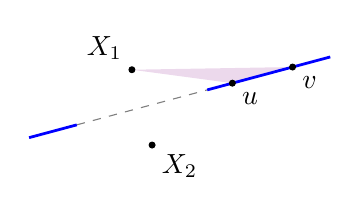
\begin{tikzpicture}[scale=0.7]
            \coordinate (C) at (1.8660254,0.5);
            \coordinate (u) at (2.3222432,0.6222432);
            \coordinate (v) at (3.4150635,0.9150635);
            \coordinate (D) at (-0.5,-0.1339746);
            \coordinate (X_1) at (0.5,0.8660254);
            \coordinate (X_2) at (0.8660254,-0.5);
            \coordinate (l) at (-1.3660254,-0.3660254);
            \coordinate (r) at (4.0980762,1.0980762);

            \fill[violet!15] (X_1) -- (u) -- (v) -- cycle;
            
            \draw[dashed, gray] (D) -- (C);
            \draw[blue, line width=1pt] (l) -- (D);
            \draw[blue, line width=1pt] (C) -- (r);

            \filldraw (u) circle (1.5pt) node[below right] {$u$};
            \filldraw (v) circle (1.5pt) node[below right] {$v$};
            \filldraw (X_1) circle (1.5pt) node[above left] {$X_1$};
            \filldraw (X_2) circle (1.5pt) node[below right] {$X_2$};
        \end{tikzpicture}
    \end{minipage}
    \begin{minipage}{0.45\textwidth}
        \centering
        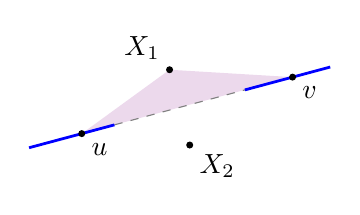
\begin{tikzpicture}[scale=0.7]
            \coordinate (C) at (1.8660254,0.5);
            \coordinate (u) at (-1.0928203,-0.2928203);
            \coordinate (v) at (2.7320508,0.7320508);
            \coordinate (D) at (-0.5,-0.1339746);
            \coordinate (X_1) at (0.5,0.8660254);
            \coordinate (X_2) at (0.8660254,-0.5);
            \coordinate (l) at (-2.0490381,-0.5490381);
            \coordinate (r) at (3.4150635,0.9150635);

            \fill[violet!15] (X_1) -- (u) -- (v) -- cycle;
            
            \draw[dashed, gray] (D) -- (C);
            \draw[blue, line width=1pt] (l) -- (D);
            \draw[blue, line width=1pt] (C) -- (r);

            \filldraw (u) circle (1.5pt) node[below right] {$u$};
            \filldraw (v) circle (1.5pt) node[below right] {$v$};
            \filldraw (X_1) circle (1.5pt) node[above left] {$X_1$};
            \filldraw (X_2) circle (1.5pt) node[below right] {$X_2$};
        \end{tikzpicture}
    \end{minipage}
    \caption{Reduction ($d=2)$ for \textsc{LocalBetweenness-Euclidean}: Type B constraints force all $v \in V$ onto two opposing rays. Left: $(u,X_1,v)$ is not satisfied when $u$ and $v$ lie on the same ray. Right: $(u,X_1,v)$ is satisfied when $u$ and $v$ lie on different rays.}
    \label{fig:betweenness-2d}
\end{figure}

% --- original figure with more readable coordinates ---

% \begin{figure}[h]
%     \centering
%     \begin{minipage}{0.45\textwidth}
%         \centering
%         \begin{tikzpicture}[scale=0.7]
%             \coordinate (C) at (1.3660254,1.3660254);
%             \coordinate (u) at (1.7,1.7);
%             \coordinate (v) at (2.5,2.5);
%             \coordinate (D) at (-0.3660254,-0.3660254);
%             \coordinate (X_1) at (0,1);
%             \coordinate (X_2) at (1,0);
%             \coordinate (l) at (-1,-1);
%             \coordinate (r) at (3,3);

%             \fill[violet!15] (X_1) -- (u) -- (v) -- cycle;
            
%             \draw[dashed, gray] (D) -- (C);
%             \draw[blue, line width=1pt] (l) -- (D);
%             \draw[blue, line width=1pt] (C) -- (r);

%             \filldraw (u) circle (1.5pt) node[below right] {$u$};
%             \filldraw (v) circle (1.5pt) node[below right] {$v$};
%             \filldraw (X_1) circle (1.5pt) node[above left] {$X_1$};
%             \filldraw (X_2) circle (1.5pt) node[below right] {$X_2$};
%         \end{tikzpicture}
%     \end{minipage}\hfill
%     \begin{minipage}{0.45\textwidth}
%         \centering
%         \begin{tikzpicture}[scale=0.7]
%             \coordinate (C) at (1.3660254,1.3660254);
%             \coordinate (u) at (-0.8,-0.8);
%             \coordinate (v) at (2,2);
%             \coordinate (D) at (-0.3660254,-0.3660254);
%             \coordinate (X_1) at (0,1);
%             \coordinate (X_2) at (1,0);
%             \coordinate (l) at (-1.5,-1.5);
%             \coordinate (r) at (2.5,2.5);

%             \fill[violet!15] (X_1) -- (u) -- (v) -- cycle;
            
%             \draw[dashed, gray] (D) -- (C);
%             \draw[blue, line width=1pt] (l) -- (D);
%             \draw[blue, line width=1pt] (C) -- (r);

%             \filldraw (u) circle (1.5pt) node[below right] {$u$};
%             \filldraw (v) circle (1.5pt) node[below right] {$v$};
%             \filldraw (X_1) circle (1.5pt) node[above left] {$X_1$};
%             \filldraw (X_2) circle (1.5pt) node[below right] {$X_2$};
%         \end{tikzpicture}
%     \end{minipage}
%     \caption{Reduction ($d=2)$ for \textsc{LocalBetweenness-Euclidean}: Type B constraints force all $v \in V$ onto two opposing rays. Left: $(u,X_1,v)$ is not satisfied when $u$ and $v$ lie on the same ray. Right: $(u,X_1,v)$ is satisfied when $u$ and $v$ lie on different rays.}
%     \label{fig:betweenness-2d}
% \end{figure}

Next, we show that in any locally maximum embedding for \textsc{LocalBetweenness-Euclidean}, a Type A constraint $(u, X_1, v)$ is satisfied if and only if $u$ and $v$ are on \textit{opposite} rays. To see this, let us analyze the triangle $\triangle u X_1 v$:
\begin{itemize}
\vspace{-0.2cm}
    \item If $u$ and $v$ are on the same ray, we have $\angle u X_1 v < 30 ^\circ$. Basic trigonometry tells us $uv$ cannot be the longest side of the triangle, thus $(u, X_1, v)$ is not satisfied.
    \vspace{-0.2cm}
    \item If $u$ and $v$ are on opposite rays, we have $\angle u X_1 v \geq 120 ^\circ$. Basic trigonometry tells us $uv$ must be the longest side of the triangle, thus $(u, X_1, v)$ is satisfied.
\end{itemize}
\vspace{-0.2cm}
Therefore, the configuration of a locally maximum embedding encodes a local max cut for $G$. We can easily recover the cut $(S,\bar{S})$ by checking whether each Type A constraint $(u, X_1, v)$ is satisfied in the configuration, e.g., $S$ can be all vertices in one ray.
\end{proof}

\iffalse
\subsection{Hardness of Embeddings on $\mathbb{R}^d$} \label{sec:embedding_in_Rd}

We begin this section by showing that $\betweeness$ is $\PLS$-hard. We prove $\PLS$-hardness through a direct $\PLS$ reduction from \textsc{Local Max-Cut/Flip}. The key idea of our reduction is to use a single point $x$ in the permutation as a ``cut'' over the one-dimension space and to construct triplet $(a_i, x, a_j)$ such that any edge across the cut contributes to the count of satisfied triplet.
% We now present the proof of $\PLS$-hardness for several discrete contrastive learning objectives. Here, ``discrete'' refers to objectives with a discrete set of values (e.g., the number of satisfied constraints), even if the solution space is continuous (e.g., $\mathbb{R}$ or $\mathbb{R}^d$).

% \subsection{Hardness of Betweenness}\label{sec:hardness-btw}

\begin{theorem}\label{thm:betweenness-1d}
Finding a local solution of \textsc{Betweenness} is $\PLS$-hard.
\end{theorem}
\begin{proof}

% \yl{Please, keep the notations consistent across the proofs. Feel free to change mine if you feel there's a better way}

% We first observe that \textsc{Betweenness} is in $\PLS$: the objective function $\score(\pi)$ is polynomial-time computable, and local moves (moving a single element to a different position) can be enumerated in polynomial time.

% It is quite clear that $\betweeness\in \PLS.$ Firstly observe that for any permutation $ p = (a_1,...,a_n)$, all local moves can be computed in polynomial time. Now consider the potential function of $p$ to be
% \[
% W(p):= \sum_{i=1}^m w_i \textbf{1}_{t_i \textrm{ is satisfied}},
% \]
% where $\textbf{1}_{t_i \textrm{ is satisfied}}$ is the indicator that $t_i$ is satisfied for the given ordering. Since $W(p)$ can be computed in polynomial time, we conclude that $\betweeness$ is in $\PLS$.

Let $G(V,E,w')$ be a weighted undirected graph with $n$ vertices $v_1,...,v_n$ for which we want to compute a local solution for $\textsc{Local Max-Cut/Flip}$. We define an instance of $\betweeness$ as follows:

We consider $n+2$ points $a_1,...,a_n, x ,y$ in which each $a_i$ represents the vertex $v_i.$ Moreover we add the following triples:

\begin{itemize}[label = ]
\item \textbf{Type A triplets}: $(x,y,a_i)$, $(y,x,a_i)$ for all $i \in [n]$ with weight $\sum_{e \in E} w'_{e}$.
\item \textbf{Type B triplets}: $(a_i,x,a_j)$ for all edges $(v_i,v_j)\in E$ with weight $w'_{(v_i,v_j)}$.
\end{itemize}

% \jy{Double check the weight for type I constraints}
% \yl{Can we remove $(a_i ,\textbf{y}, a_j)$?}

Type A triplets ensure that in any local solution there will be no points between $x$ and $y$. To see it, assume that $x$ is to the left of $y$ and consider an ordering where point $a_i$ is the leftmost point between $x$ and $y.$ By moving $a_i$ one position on the left, triplets $(x,y,a_i)$ and $(y,x,a_i)$ become satisfied (which were not satisfied previously). Let $\calS_{\text{left}}$ denote the set of indices of points that were originally to the left of $x$. For any $j \in \calS_{\text{left}}$,  the triplet $(a_j, x, a_i)$ is no longer satisfied after the move. As a result, the objective will increase by $2 \sum_{e \in E} w'_{e} - \sum_{j \in \calS_{\text{left}}} w'(v_i, v_j) + \sum_{k \notin \calS_{\text{left}}} w'(v_i, v_k) > 0$. Thus we conclude that any solution of $\betweeness$ must be an ordering for which there are no points between $x$ and $y.$ Furthermore, since the weight of triplets $(x, y, a_i)$ and $(y, x, a_i)$ is greater than the summed weight $(a_i, x, a_j)$ for all pair $(i, j)$ such that $ i \neq j$, $x$ can not deviate away from $y$. 

Given any ordering that satisfies all the Type A triples, we create a cut of the graph $G$ as follows. The left partition of $G$ will be all the vertices $v_i$ whose representatives $a_i$ are positioned on the left of $x,y$ and the right partition of $G$ will be the remaining vertices. Note that Type B constraint $(a_i, x, a_j)$ can only be satisfied if $a_i$ and $a_j$ are on different side of $x$.

We conclude that given any ordering of $a_1, \dots, a_n, x, y$ satisfying all Type A triplets, one can construct a cut in $G$. Moreover, the potential $W$ computed for a given ordering that satisfies all Type A triples is equal to twice the size of the cut that is induced by that ordering. As a result, any local maximum of $W$ should be a local max-cut of $G.$ The result follows since the reduction is of polynomial time.

\jy{Make sure the notation of this potential matches other notations, here temporarily we are using $W$.}

% \yl{local max cut definition here: We prove $\PLS$-hardness by a $\PLS$ reduction from \textsc{Max-Cut/Flip}, which is known to be $\PLS$-complete~\citep{schaffer1991simple}. Given a weighted undirected graph $G = (V, E, w)$ with $n$ vertices, the goal in \textsc{Max-Cut/Flip} is to partition $V$ into two sides to maximize the total weight of crossing edges, where a local move ``flips'' the color of a single vertex, i.e., moves it from one side to the other.}

% We construct an instance of \textsc{Betweenness} as follows. Let the set of elements be $V' = V \cup \{X, Y\}$, where $X$ and $Y$ are two special elements defining the cut boundary.

% \yl{I think we only need $X$. We allow moving $X$ because it still satisfies ``any locally optimal ordering is a locally optimal cut,'' even if it is not a one-to-one mapping.}
\end{proof}

\jy{Sorry I didn't realize yiyuan has written down one version of the proof, feel free to use any of the two version as long as notation matches.}

\begin{proof}
    

% \begin{remark}
    
% \end{remark}

We define two types of \textsc{Betweenness} constraints:

\textbf{Type A (Edge Constraints).} For every edge $(u, v) \in E$ with weight $w_{uv}$, add a single constraint $(u, X, v)$ with weight $w_{uv}$.

\textbf{Type B (Boundary Constraints).} For every $v \in V$, add two constraints $(X, Y, v)$ and $(Y, X, v)$, each with weight
\[
M = \sum_{(u,v) \in E} w_{uv} + 1.
\]

To give some intuition, we first show that in any local optimum $X$ and $Y$ are adjacent. Consider if any $v \in V$ is placed between $X$ and $Y$, moving it to either side increases the score by $M$, while at most losing the total weight of incident Type A constraints (at most $\sum w_{uv}$), meaning that this configuration cannot be locally optimal.

Once $X$ and $Y$ are adjacent, the ordering encodes a cut of $G$: vertices to the left of $\{X, Y\}$ form one side of the cut, vertices to the right form the other side. Under this configuration, observe that the Type A constraint $(u, X, v)$ is satisfied if and only if $u$ and $v$ are on opposite sides of $\{X, Y\}$. Moving a vertex $v$ across $X$ and $Y$ flips its side in the cut, changing the \textsc{Betweenness} score by the same amount as the cut weight change in \textsc{Max-Cut/Flip}. Since local moves and changes correspond exactly, a locally optimal ordering corresponds to a locally optimal cut.
\end{proof}


% \vnote{hi Yiyuan, can we have the d=2 case separately so that it's easier to convince the reviewer? Thanks!}

% \yl{I'm trying to finish the general case first ans see how long it is. If it's too long I'll make a d=2 version and put the rest into appendix}

% \vnote{sure no worries :)}

\begin{theorem}\label{thm:betweenness-high}
For every fixed $d \geq 2$, finding a local optimum of \textsc{Betweenness} in $\mathbb{R}^d$ is $\PLS$-hard.
\end{theorem}

We first prove \textsc{Betweenness} on a 2D plane is $\PLS$-hard. We generalize the reduction to higher dimensions in Appendix~\ref{app:betweenness-high}.

\begin{proof}
We give a $\PLS$ reduction from \textsc{Max-Cut/Flip}.
Let $G = (V, E, w)$ be a weighted undirected graph. We construct an instance of \textsc{Betweenness-2D} as follows. We introduce special elements $X_1$ and $X_2$ and add two types of constraints:

\item \textbf{Type A (Edge Constraints).}
For each edge $(u, v) \in E$ with weight $w_{uv}$, add a single constraint $(u, X_1, v)$ with weight $w_{uv}$.

\item \textbf{Type B (Isosceles Constraints).}
For each $v \in V$, add two constraints $(X_1, X_2, v)$ and $(X_2, X_1, v)$, each with weight $M = \sum_{(u,v) \in E} w_{uv} + 1$.
Intuitively, this will force $X_1, X_2, v$ to form an \emph{isosceles triangle} such that $\| v - X_1 \| = \| v - X_2 \| \geq \| X_1 - X_2 \|$.

Observe that in any local optimum, all Type B constraints must be satisfied. If any Type B constraint involving $v$ is unsatisfied, we can always satisfy it by moving $v$ to form an isosceles triangle such that $\|v - X_1\| = \|v - X_2\| \geq \|X_1 - X_2\|$, gaining at least $M$ while losing at most $\sum w_{uv} < M$, which strictly increases the score. This effectively forces $v$ to lie on one of two rays (see Figure \ref{fig:betweenness-2d}).

\begin{figure}[h]
    \centering
    \begin{minipage}{0.45\textwidth}
        \centering
        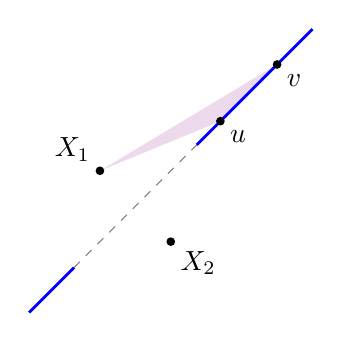
\begin{tikzpicture}[scale=0.9]
            \coordinate (C) at (1.3660254,1.3660254);
            \coordinate (u) at (1.7,1.7);
            \coordinate (v) at (2.5,2.5);
            \coordinate (D) at (-0.3660254,-0.3660254);
            \coordinate (X_1) at (0,1);
            \coordinate (X_2) at (1,0);
            \coordinate (l) at (-1,-1);
            \coordinate (r) at (3,3);

            \fill[violet!15] (X_1) -- (u) -- (v) -- cycle;
            
            \draw[dashed, gray] (D) -- (C);
            \draw[blue, line width=1pt] (l) -- (D);
            \draw[blue, line width=1pt] (C) -- (r);

            \filldraw (u) circle (1.5pt) node[below right] {$u$};
            \filldraw (v) circle (1.5pt) node[below right] {$v$};
            \filldraw (X_1) circle (1.5pt) node[above left] {$X_1$};
            \filldraw (X_2) circle (1.5pt) node[below right] {$X_2$};
        \end{tikzpicture}
    \end{minipage}\hfill
    \begin{minipage}{0.45\textwidth}
        \centering
        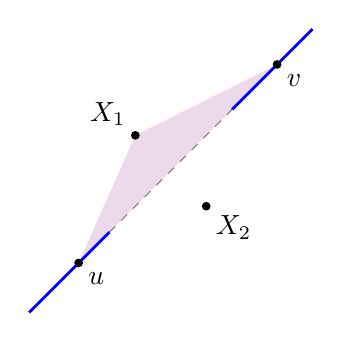
\begin{tikzpicture}[scale=0.9]
            \coordinate (C) at (1.3660254,1.3660254);
            \coordinate (u) at (-0.8,-0.8);
            \coordinate (v) at (2,2);
            \coordinate (D) at (-0.3660254,-0.3660254);
            \coordinate (X_1) at (0,1);
            \coordinate (X_2) at (1,0);
            \coordinate (l) at (-1.5,-1.5);
            \coordinate (r) at (2.5,2.5);

            \fill[violet!15] (X_1) -- (u) -- (v) -- cycle;
            
            \draw[dashed, gray] (D) -- (C);
            \draw[blue, line width=1pt] (l) -- (D);
            \draw[blue, line width=1pt] (C) -- (r);

            \filldraw (u) circle (1.5pt) node[below right] {$u$};
            \filldraw (v) circle (1.5pt) node[below right] {$v$};
            \filldraw (X_1) circle (1.5pt) node[above left] {$X_1$};
            \filldraw (X_2) circle (1.5pt) node[below right] {$X_2$};
        \end{tikzpicture}
    \end{minipage}
    \caption{$\textsc{Betweenness-2D}$ reduction. Type B constraints force all $v \in V$ onto two opposing rays. Left: $(u,X_1,v)$ is not satisfied when $u$ and $v$ lie on the same ray. Right: $(u,X_1,v)$ is satisfied when $u$ and $v$ lie on different rays.}
    \label{fig:betweenness-2d}
\end{figure}

\yl{the guideline says the table must be centered, but didn't say figures should. I think putting a figure on the side of the text is allowed. I'm not very familiar with how to use \{wrapfigure\} (I made some unsuccessful attempts). If any of you know how and think we need that, please feel free to do it.}

We show that in any local optimum, a Type A constraint $(u, X_1, v)$ is satisfied if and only if $u$ and $v$ are on opposite rays. Analyze triangle $\triangle u X_1 v$:
\begin{itemize}
    \item If $u$ and $v$ are on the same ray, we have $\angle u X_1 v < 30 ^\circ$. Basic trigonometry tells us $uv$ cannot be the longest side of the triangle, thus $(u, X_1, v)$ is not satisfied.
    \item If $u$ and $v$ are on opposite rays, we have $\angle u X_1 v \geq 120 ^\circ$. Basic trigonometry tells us $uv$ must be the longest side of the triangle, thus $(u, X_1, v)$ is satisfied.
\end{itemize}

Therefore, the configuration encodes a cut, while preserving the local optimality. We can easily recover the cut by checking whether each Type A constraint $(u, X_1, v)$ is satisfied in the configuration.
\end{proof}

% \yl{Please, read this. I believe the following is a quick fix to make my reduction follow the assumption that no two points overlap. We don't add the constraint $(X_l, a_i, X_k)$. In other words, instead of making $a_i, X_l, X_k$ an equilateral triangle, we only need to make $a_i, X_l, X_k$ form an isosceles triangle such that $\dist(a_i, X_l) = \dist(a_i, X_k) \geq \dist(X_l, X_k)$. Then we have $a_i = (\alpha, \dots, \alpha) \in \mathbb{R}^d$ where $\alpha \geq \frac{1 + \sqrt{d + 1}}{d}$ or $\alpha \leq \frac{1 - \sqrt{d + 1}}{d}$ (two rays). And we can show that $(a_i, X_1, a_j)$ is satisfied iff $a_i$ and $a_j$ are not on the same ray. This reduction still holds with the $[0,1]^d$ box, as long as we scale the simplex to an appropriate size and then translate it to an appropriate position. This might be the optimal solution to the problem: based on the assumption ``points don't overlap'', we don't need any fixed points.}
\iffalse
\begin{theorem}\label{thm:contrastive-1d}
Finding a local optimum of \textsc{Contrastive-1D} is $\PLS$-complete.
\end{theorem}

\begin{proof}

\textbf{Membership in $\PLS$.}
While the solution space is continuous, we argue that the objective function is piecewise constant over a finite subdivision of $\mathbb{R}^n$. Specifically, each constraint $(x, y^+, z^-)$ depends on the sign of $|x - y| - |x - z|$, which changes only at one or two critical points over $\mathbb{R}$. Moving a single element only affects the constraints involving that element, partitioning the real line into at most $O(m)$ intervals, which can be enumerated efficiently. Evaluating the score in each interval is polynomial-time, so a best local move can be computed in polynomial time.

\textbf{Reduction from \textsc{Max-Cut/Flip}.} Let $G = (V, E, w)$ be a weighted undirected graph. We construct an instance of \textsc{Contrastive-1D} as follows. We introduce special elements $X, Y, Z$ and add constraints as the following:

\textbf{Type A (Edge Constraints).} For every edge $(u, v) \in E$ with weight $w_{uv}$, add a single constraint $(u, X^+, v^-)$ with weight $w_{uv}$.

\textbf{Type B (Boundary Constraints).} We add the following:
\begin{itemize}
    \item $(X, Y^+, v^-)$ with weight $M = \sum_{(u,v) \in E} w_{uv} + 1$ for every $v \in V$.
    \item $(X, v^+, Z^-)$ with weight $M$ for every $v \in V$.
    \item $(Y, Z^+, X^-)$ with weight $M' = (2 |V| + 1)M$.
    \item $(X, Y^+, Z^-)$ with weight $M'$.
\end{itemize}

We show that in any local optimum, $(X, Y^+, Z^-)$ and $(Y, Z^+, X^-)$ are satisfied, therefore $X, Y, Z$ must ordered as $X < Y < Z$ or $Z < Y < X$, and moreover, $|X - Y| \geq |Y - Z|$. If any of those two constraints is unsatisfied, we can always satisfy both simultaneously by moving $Z$, gaining at least $M'$ while losing at most $2 |V| M + \sum_{(u,v) \in E} w_{uv} < M'$, which contradicts local optimality.

We next show in any local optimum, all $(X, Y^+, v^-)$ and $(X, v^+, Z^-)$ are satisfied, meaning that each $v \in V$ must lie on one of two segments $YZ$ or $Y'Z'$, where $Y'$ and $Z'$ are the reflections of $Y$ and $Z$ w.r.t. $X$ respectively (see Figure \ref{fig:contrastive-1d}). If any $(X, Y^+, v^-)$ or $(X, v^+, Z^-)$ is unsatisfied, we can always satisfy both by moving $v$ to $YZ$ or $Y'Z'$, gaining at least $M$ while losing at most $\sum_{(u,v) \in E} w_{uv} < M$.

% \yl{very small bug: $Y'$ and $Z'$ are virtual (not occupying the position), so points can be placed on these endpoints to cheat. introduce real $Y'$ and $Z'$}

\begin{figure}[h]
    \centering
    
\begin{tikzpicture}
        \coordinate (Z') at (-3,0);
        \coordinate (Y') at (-2,0);
        \coordinate (X) at (0,0);
        \coordinate (Y) at (2,0);
        \coordinate (Z) at (3,0);
        \coordinate (l) at (-5,0);
        \coordinate (r) at (5,0);
        
        \draw[dashed, gray] (l) -- (Z');
        \draw[blue, line width=1pt] (Z') -- (Y');
        \draw[dashed, gray] (Y') -- (Y);
        \draw[blue, line width=1pt] (Y) -- (Z);
        \draw[dashed, gray] (Z) -- (r);
        
        \filldraw (Z') circle (1.5pt) node[above] {$Z'$};
        \filldraw (Y') circle (1.5pt) node[above] {$Y'$};
        \filldraw (X) circle (1.5pt) node[above] {$X$};
        \filldraw (Y) circle (1.5pt) node[above] {$Y$};
        \filldraw (Z) circle (1.5pt) node[above] {$Z$};
    \end{tikzpicture}
    \caption{$\textsc{Contrastive-1D}$ reduction. In any local optimum, all $v \in V$ are on either $YZ$ or $Y'Z'$.}
    \label{fig:contrastive-1d}
\end{figure}

Finally, it is clear that $(u, X^+, v^-)$ is satisfied if and only if $u$ and $v$ are on different sides of $X$. This encodes a cut and preserves local optimality.
\end{proof}
\fi
\begin{theorem}\label{thm:contrastive-high}
For every fixed $d \geq 2$, finding a local optimum of \textsc{Contrastive-$d$} is $\PLS$-hard.
\end{theorem}

\begin{proof}
\yl{not a final version, 95\% done}

We extend the reduction for \textsc{Contrastive-1D} to higher dimensions by modifying the \textsc{Betweenness-$d$} construction in Appendix~\ref{app:betweenness-high}.

Recall that in the \textsc{Betweenness-$d$} construction, all $v \in V$ are forced onto two opposing rays extending from the center of a regular simplex formed by $X_1, \dots, X_d$.

To turn these rays into segments, we do the following.

Let $Z$ be a point on the so-called "ray," and $Y$ be a point forming an equilateral triangle with $X_1$ and $X_2$. The constraint $(Y, Z^+, X_1^-)$ ensures that $\|Z - Y\| \leq \|X_1 - Y\|$, so $YZ$ is the segment we ``cut'' on the ray.

For a point $v$, $(X_1, Y^+, v^-)$ and $(X_1, v^+, Z^-)$ ensure that $v$ is on $YZ$, or on its mirror $Y'Z'$ with respect to $X_1 X_2$.

The same construction applies in higher dimensions.
\end{proof}

\begin{figure}[h]
    \centering
    \begin{tikzpicture}[scale=1.1]
        \coordinate (Y) at (1.3660254,1.3660254);
        \coordinate (Y') at (-0.3660254,-0.3660254);
        \coordinate (Z) at (1.8,1.8);
        \coordinate (Z') at (-0.8,-0.8);
        \coordinate (X_1) at (0,1);
        \coordinate (X_2) at (1,0);
        \coordinate (l) at (-1.5,-1.5);
        \coordinate (r) at (2.5,2.5);
        
        \draw[dashed, gray] (l) -- (Z');
        \draw[blue, line width=1pt] (Z') -- (Y');
        \draw[dashed, gray] (Y') -- (Y);
        \draw[blue, line width=1pt] (Y) -- (Z);
        \draw[dashed, gray] (Z) -- (r);

        \filldraw (Y) circle (1.5pt) node[below right] {$Y$};
        \filldraw (Y') circle (1.5pt) node[below right] {$Y'$};
        \filldraw (Z) circle (1.5pt) node[below right] {$Z$};
        \filldraw (Z') circle (1.5pt) node[below right] {$Z'$};
        \filldraw (X_1) circle (1.5pt) node[above left] {$X_1$};
        \filldraw (X_2) circle (1.5pt) node[below right] {$X_2$};
    \end{tikzpicture}
    \caption{$\textsc{Contrastive-2D}$ reduction. In any local optimum, all $v \in V$ are on either $ZA$ or $Z'A'$.}
    \label{fig:contrastive-2d}
\end{figure}


% \jy{This should be betweenness problem, contrastive problem is defined to be the one with continuous objective}






% \yl{For Contrastive, we can slightly modify the above reduction to restrict all $a_i$s to two short segments to make the reduction from max-cut work (Find a point $I$ on one ray within the hypersphere centered at $J$ with radius $||JA$||, then let all $a_i$ be within the hypersphere centered at $A$ with radius $||AI||$. See figure~\ref{fig:2d-contrastive}).}

% \begin{figure}
%     \centering
%     \includegraphics[width=0.8\linewidth]{figure/2d_contrastive_pro_max.png}
%     \caption{Fancy Figure Needed}
%     \label{fig:2d-contrastive}
% \end{figure}

% \yl{give it a more precise name; point out the difference in settings: here we do not have the restriction that $a_i \in [0,1]^d$ (the box constraints), and we allow overlapping (multiple points can be at the same position). However, the advantage is that we only need two fixed points. This may suggest a more general case, need to check.}

% \yl{I have a much simpler reduction that only needs two reference points: $X(1,0)$ and $Y(0,1)$. If we add constraints $(X,Y,a_i), (X,a_i,Y), (a_i,X,Y)$ (each with a large weight to enforce satisfaction), then $a_i, x, y$ must form an equilateral triangle. At this point, $a_i$ can only be at two points: $\left( \frac{1 + \sqrt{3}}{2}, \frac{1 + \sqrt{3}}{2} \right)$ or $\left( \frac{1 - \sqrt{3}}{2}, \frac{1 - \sqrt{3}}{2} \right)$. Then, for each edge $i - j$ in the graph, add constraint $(a_i, X, a_j)$ with weight $w_{ij}$. This way, if $a_i$ and $a_j$ are not at the same point, you get a reward of $w_{ij}$.}

% \yl{Extend to $d$-dimensional space: Let's first consider a 3D space. Fix $X(1,0,0)$, $Y(0,1,0)$. We can add a point $Z$ to form an equilateral triangle with $X$ and $Y$. Then force all $a_i$ to form equilateral triangles with $X$, $Y$, $Z$. This way, $a_i$ only has two possible positions (relative to the position of $Z$). For $d$-dimensional space, we actually first construct a $d-1$ dimensional regular simplex (which has $d$ points). WLOG assume these $d$ points are $(1, 0, 0, ... , 0)$, $(0, 1, 0, ..., 0)$, ..., $(0, 0, 0, ..., 1)$. Then we force each $a_i$ forms a $d$-dimensional regular simplex with these points, so $a_i$ has only two choices: $a_i = (\alpha, \dots, \alpha) \in \mathbb{R}^d$ where $\alpha = \frac{1 \pm \sqrt{d + 1}}{d}$. The distance between these two different choices is $2 \sqrt{\frac{d+1}{d}} > 2 > \sqrt{2}$, so we can safely add the constraint $(a_i, X, a_j)$.}

% \yl{For discrete contrastive learning-1D: Fix $X(0)$, $Y(1)$, Add $(X, Y, a_i)$, $(X, a_i, Y)$ with large weight $\Rightarrow a_i = 1 \text{ or } a_i = -1$; Add $(a_i, X, a_j)$ with weight $w_{ij}$}

\yl{One thing needs to clarify is that we can (??) reduce from Betweenness to Contrastive (a Betweenness triplet $(a_i,a_j,a_k)$ = two Contrastive triplets $(a_i,a_j,a_k)$ and $(a_k,a_j,a_i)$) (this also needs to check). The reverse is not obvious. In other words, I don't believe the following proof implies Betweenness is PLS-hard.}

\fi
\subsection{Hardness of tree embeddings}\label{sec:hardness-tree}

% \jy{Add formal proof in the appendix}
%In this section we show the complexity result of triplets. Specifically, we show the following theorem.

% We firstly define the triplet constraint, following the notion as in \citep{chatziafratis2023triplet}.

% \begin{definition}[Triplets]
%     A rooted, unordered, binary tree $T$ is said to satisfy triplet $t = ab|c$ if the Lowest Common Ancestor of $a$ and $b$, $LCA(a, b)$, is a proper descendant of $LCA(a, c)$ in $T$. Generally, each triplet $t_i$ can have positive weight $w_i$.
% \end{definition}

% We proceed to introduce the $\Triplets$ problem.

% \begin{nproblem}[\Triplets]
%  \textsc{Input:}  
%  \begin{itemize}
%    \item A collection of $n$ real numbers $a_1,\dots,a_n$.
%    \item A collection of $m$ triples $t_1,\dots, t_{m}$ with positive weights $w_1,\dots, w_{m}$. Each triplet is defined on three points in $\{a_1, \dots, a_n\}$.
% \end{itemize}

%   \noindent \textsc{Output:} A hierarchical clustering (i.e. the binary rooted tree) $T$ that maximize the utility $\sum_{i = 1}^m w_i \cdot \mathbb{I}(T \text{ satisfies } t_i)$.
% \end{nproblem}

% \jy{need to define the local moves here}

% We are ready to show the main result for this section.
\begin{theorem}\label{thm:local-contrastive-tree}
The \textsc{LocalContrastive-Tree} problem is $\PLS$-hard.
\end{theorem}
\vspace{-0.2cm}
\begin{proof}[Proof Sketch.]
    
We do a $\PLS$-reduction from \textsc{LocalMaxCut}. Given graph $G(V, E)$, we construct triplets over nodes $V\cup \{X, X', Y, Z\}$ for special nodes $\{X, X', Y, Z\}$. The triplets are as follows:
    \begin{itemize}
    \vspace{-0.2cm}
        \item \textbf{Type A triplets}: $XX'|Y$, $XX'|Z$, and $XX'|v$ for all $v \in V$, each with weight $\sum_{e \in E}w_e$
        \vspace{-0.2cm}
        \item \textbf{Type B triplets}: $XY|Z$ with a large weight $|V| \cdot \sum_{e \in E}w_e + |V| + 1$
        \vspace{-0.2cm}
        \item \textbf{Type C triplets}: $Yv|X$ and $Zv|X$ for all $v \in V$, each with weight $\sum_{e \in E}w_e + 1$
        \vspace{-0.2cm}
        \item \textbf{Type D triplets}: $uX|v$ and $vX|u$ whenever $(u, v) \in E$, each with weight $w_{uv}/2$
        \vspace{-0.2cm}
    \end{itemize}
    The purpose of the special vertices and the constraints is that they force the tree to look as in \Cref{fig:triplet}: $X,X'$ are siblings, and any other vertex $v\in V$ is either in subtree $T_Y$ containing $Y$ or subtree $T_Z$ containing $Z$ (because of heavy Type C triplets). Then, the solution to \textsc{LocalMaxCut} can be formed by all nodes that fell in $T_Y$ as one side of the cut, and to $T_Z$ as the other side. The proof proceeds by a case analysis showing that this is indeed a local max cut, and that no vertex can increase the weight of the cut edges by moving to the other subtree (for full proof, see~\Cref{sec:proof_hardness_tree}).
    \end{proof}

    %We proceed to show that for any pair of points $a_i$ and $a_j$, where $i \neq j $ and $i, j \in [0, 1]$, if $a_i$ and $a_j$ are on the same branch (either the branch with $y$ or the branch with $z$), then neither of $a_ix|a_j$ or $a_jx|a_i$ would be satisfied. If $a_i$ and $a_j$ are on different branches, assuming that $a_i$ is on the branch of $y$ and $a_j$ is on the branch of $z$, then triplet $a_ix|a_j$ with weight $w(v_i, v_j)$ would be satisfied. Since for all $i \in [1, n]$, $a_i$ can only reside in either the branch of $y$ or the branch of $z$, we conclude that in any local solution $T$, the configuration of all $a_i$ will introduce a local max cut of the original graph. That is, for any $i \in [1, n]$, if $a_i$ is on the branch of $y$, then the corresponding vertex $v_i$ would be on one side of the cut. If $a_j$ is on the branch of $z$, then the corresponding vertex $v_j$ would be on the other side of the cut. The proof is complete.

    % \jy{I don't think we need to argue about x moving in this case because above analysis holds for any local solution.}




\iffalse
\begin{proof}
    % Since the potential function for any configuration $a_1, \dots, a_n, x, x', y, z$ can be written as
    % \begin{align}
    %     W(a_1, \dots, a_n):= \sum_{k=1}^m w_k \textbf{1}_{t_k \textrm{ is satisfied}},
    % \end{align}
    % we conclude that local $\Triplets \in \PLS$.

    \yl{refine the comparison of weights, instead of saying ``... dominates.'' check if we need hierarchy}
    
    The hardness result can be derived from a direct reduction from local max-cut to the local solution of $\Triplets$. For a given graph $G(V, E, w)$ where $V = {v_1, \dots, v_n}$, we construct the triplets over nodes $\{a_1, \dots, a_n, x, x', y, z\}$ where each node $a_i$ represents vertex $v_i \in V$. The triplets are constructed as
    \begin{itemize}
        \item \textbf{Type A triplets}: $xx'|y$, $xx'|z$, and $xx'|a_i$ for all $i \in [1, n]$, each with weight $\sum_{e \in E}w(e)$;
        \item \textbf{Type B triplets}: $xy|z$ with a large weight $n \sum_{e \in E}w(e)$;
        \item \textbf{Type C triplets}: $ya_i|x$ and $za_i|x$ for all $i \in [1, n]$, each with weight $\sum_{e \in E}w(e);$
        \item \textbf{Type D triplets}: $a_ix|a_j$ and $a_jx|a_i$ for any $i, j$ pairs such that $(v_i, v_j) \in E$, each with weight $w(v_i, v_j)$.
    \end{itemize}
    Assume that $T$ is a local solution of the above triplets instance. Since $T$ is an rooted binary tree, there exists a unique path $p$ starting from the leave node $x$ to the root. All other leave nodes $\{a_1, \dots, a_n, x', y, z\}$ would be on branches of this path $p$. Firstly observe that $x'$ should share the same parent node with $x$. In other words, $x'$, and only $x'$, should be on the lowest branch on the path $p$. If this is not the case, $x'$ can simply move to a location such that $x$ and $x'$ share the same parent node and this would only increase the satisfied triplets by satisfying all triplets of Type A.
    
    Since in any local solution $T$, Type A triplets are always satisfied as argued above. For nodes $y$ and $z$, Type B triplet $xy|z$ has dominating weight (the weight of $xy|z$ is greater than the sum of weights of other triplets that $y$ or $z$ is involved). Thus any local solution $T$ needs to satisfy Type B triplet. We note that the triplet $xy|z$ can only be satisfied when $y$ is on a lower branch of $z$ on the path $p$. 

    Similarly for each $a_i$, triplets $ya_i|x$ and $za_i|x$ have dominating weights. Thus in any local solution $T$, $a_i$ would try to satisfy $ya_i|x$ and $za_i|x$ first. Since $y$ and $z$ are on different branch, for each $a_i$, only one of the two triplets above could be satisfied in a local solution $T$. Notice that in order to satisfy $ya_i|x$ or $za_i|x$, node $a_i$ should be on the branch of $y$ or the branch of $z$ respectively. We conclude that in a local solution $T$, for any $i \in [1, n]$, $a_i$ should be on either the branch with point $y$ or the branch of point $z$.

    We proceed to show that for any pair of points $a_i$ and $a_j$, where $i \neq j $ and $i, j \in [0, 1]$, if $a_i$ and $a_j$ are on the same branch (either the branch with $y$ or the branch with $z$), then neither of $a_ix|a_j$ or $a_jx|a_i$ would be satisfied. If $a_i$ and $a_j$ are on different branches, assuming that $a_i$ is on the branch of $y$ and $a_j$ is on the branch of $z$, then triplet $a_ix|a_j$ with weight $w(v_i, v_j)$ would be satisfied. Since for all $i \in [1, n]$, $a_i$ can only reside in either the branch of $y$ or the branch of $z$, we conclude that in any local solution $T$, the configuration of all $a_i$ will introduce a local max cut of the original graph. That is, for any $i \in [1, n]$, if $a_i$ is on the branch of $y$, then the corresponding vertex $v_i$ would be on one side of the cut. If $a_j$ is on the branch of $z$, then the corresponding vertex $v_j$ would be on the other side of the cut. The proof is complete.

    % \jy{I don't think we need to argue about x moving in this case because above analysis holds for any local solution.}
    
\end{proof}
\fi

\begin{figure}[ht]
    \centering
    \begin{tikzpicture}[scale = 0.8,
        leaf/.style={
            draw,
            dashed,
            isosceles triangle,
            isosceles triangle apex angle=60,
            shape border rotate=90,
            minimum height=1.6cm,
            anchor=apex
        },
        note/.style={draw=none, rectangle, align=center},
        line width=0.5pt
    ]
    
    \coordinate (root) at (0,0);
    \coordinate (a) at (-2.3,-2);
    \coordinate (b) at (-4,-4);
    \coordinate (x) at (-4.3,-4.7);
    \coordinate (x') at (-3.7,-4.7);
    
    % labels
    \node[anchor=base] at (-4.4,-5.2) {$X$};
    \node[anchor=base] at (-3.7,-5.2) {$X'$};
    \node[anchor=base] at (-1.2,-4.3) {$Y$};
    \node[anchor=base] at (1.5,-2.3) {$Z$};
    
    \filldraw (x) circle (1.5pt);
    \filldraw (x') circle (1.5pt);
    \filldraw (-1.5,-4.1) circle (1.5pt);  % Y
    \filldraw (1.25,-2.1) circle (1.5pt);  % Z

    % \node at (-1.2,-4.5) {\LARGE $A$};
    % \node at (1.5,-2.5) {\LARGE $B$};
    
    \node[leaf] (y) at (-1.2,-3) {};
    \node[leaf] (z) at (1.5,-1) {};
    
    \draw (root.center) -- (z.apex);
    \draw (root.center) -- (a.center);
    \draw (a.center) -- (y.apex);
    \draw (a.center) -- (b.center);
    \draw (b.center) -- (x);
    \draw (b.center) -- (x');
    \end{tikzpicture}
    \caption{Reduction for \textsc{LocalContrastive-Tree}.}
    \label{fig:triplet}
\end{figure}
\section{\texorpdfstring{$\CLS$}{CLS}-hardness for continuous objectives in contrastive learning}\label{sec:hardness-cls}
%In this section we present the result indicating that $\Contrastive$ is hard, namely $\CLS$-hard. 

% We consider the following problem

% \begin{nproblem}[\Contrastive]
%  \textsc{Input:}  
%  A collection of $n$ real numbers $a_1,\dots,a_n \in [0, 1]$ and the following $4$ types of constraints.
%  \begin{itemize}
%    \item A collection of $m_1 < n^3$ triples $t_1,\dots, t_{m_1}$ with positive weights $w_1,\dots, w_{m_1}$. Each triplet is of the form $(a_i,a_j,a_k)$ and is satisfied as long as the distance between $a_i$ and $a_j$ is smaller than the distance between $a_i$ and $a_k$.
%    \item A collection of $m_2 < n^2$ triplets $t_{m_1 + 1}, \dots, t_{m_1 + m_2},$ with positive weights $w_{m_1 + 1},\dots,w_{m_1 + m2}$. Each triplet is of the form $(a_i, 0,  a_j)$ and is satisfied as long as the distance between $a_i$ and $0$ is smaller than the distance between $a_i$ and $a_j$. 
%    \item A collection of $m_3 < n$ triplets $t_{m_1 + m_2+1}, \dots , t_{m_1 + m_2 + m_3}$ with positive weights $w_{m_1 + m_2 + 1}$ , $\dots$ ,$w_{m_1 + m_2 + m_3}$. Each triplet is of the form $(a_i, 0, 1)$ and is satisfied as long as the distance between $a_i$ and $0$ is smaller than the distance between $a_i$ and $1$. 
%    \item A collection of $m_4 < n$ triplets $t_{m_1 + m_2+ m_3 + 1}$ , $\dots$, $t_{m_1 + m_2 + m_3 + m_4}$ with positive weights $w_{m_1 + m_2 + m+3 + 1}, \dots ,w_{m_1 + m_2 + m_3 + m_4}$. Each triplet is of the form $(a_i, 1, 0)$ and is satisfied as long as the distance between $a_i$ and $1$ is smaller than the distance between $a_i$ and $0$. 
% \end{itemize}

%   \noindent \textsc{Goal:} Compute a permutation  $a_1',...,a_n'$ that minimizes $\sum_{i = 1}^{m_1+ m_2 + m_3 + m_4} w_i t_i$ . 
% \end{nproblem}

% Any constraints $(a_i, a_j, a_k)$ with weight $w$ would induce the following cost function
% \begin{align}
%     w\left((a_i - a_j)^2 - (a_i - a_k)^2\right).
% \end{align}
% For any constraints $(a_i, a_j, a_k),$ we denote the constraint $(a_i, a_k, a_j)$ as its dual constraint. Notice with weight $w$ on $(a_i, a_j, a_k)$ and weight $w'$ on the dual constraint $(a_i, a_k, a_j)$, we have the following cost function
% \begin{align}
%     (w - w')\left((a_i - a_j)^2 - (a_i - a_k)^2\right).
% \end{align}
% We proceed to show the local solution \Contrastive problem is $\CLS$-hard. Unlike \betweeness problem where only the ordering of the points matters, in \Contrastive problem we introduce two \textit{pivot} points, namely $0$ and $1$. We note that without the pivot points, the \Contrastive problem has a trivial solution, where $a_1 = a_2 = \cdots = a_n.$ If we only have one \textit{pivot} point, we can simply set all points $a_1 = \dots = a_n$ to be equal to the pivot point and achieve a local solution. Thus we deem introducing two \textit{pivot} point $0$ and $1$ is necessary to make the problem non-trivial.

\begin{theorem} \label{thm:CLS_hard_contrastive}
For every dimension $d\ge1$, \textsc{LocalTripletLoss-Euclidean} is $\CLS$-hard. 
\end{theorem}
\begin{proof}[Proof Sketch] We present the key idea for the case $d=1$ with two pivot points $A = 0$ and $B = 1/2$. The full proof is in \Cref{sec:omitted_proof_contrastive}. 
We give a $\CLS$-reduction from \textsc{QuadraticProgram-KKT}. The key idea is that we can use triplets of the form $(x, y, z)$ to simulate the quadratic function. For now, imagine we had as a representation function $f(\cdot)$ the identity function. Then, a given triplet constraint $(x, y, z)$ with weight $w$ will contribute the following term to the overall Triplet Loss:
\begin{align*}
    \mathcal{L}(x,y,z) = w \cdot \max\{(x - y)^2 - (x - z)^2 + \alpha, 0\}
\end{align*}
Our proof first breaks the given quadratic program into smaller quadratics on three variables at a time:
\[
q(x, y, z) \coloneqq c_1 x^2 + c_2 y^2 + c_3 z^2 + c_4 xy + c_5 xz + c_6 yz + c_7 x + c_8 y + c_9 z
\]
We then show how to generate a set of $m$ carefully chosen triplets $\{(x_i, y_i, z_i)\}_{i=1}^m$ with appropriate weights $w_i$ so that the total triplet loss $\mathcal{L}$ is the same as the quadratic program. It is easy to see that for terms depending only on one variable such as $c_1x^2$ or $c_8 y$, we can easily generate them by using a triplet (for example, triplet $(0, x, \frac{1}{2})$ allows us to generate the quadratic term $x^2$ and triplet $(y, 0, \frac{1}{2})$ generates the linear term $y$). However, the main obstacle is that  for the cross-terms like $xy$ we need to use triplet $(x,0,y)$, and this introduces dependencies among the different triplets since there are shared variables. To overcome the difficulty of interacting terms, we need to introduce a total of $12$ contrastive triplets on $x,y,z$, whose corresponding weights depend on the coefficients of the given quadratic. By solving a linear system for the weights, we obtain a loss $\mathcal{L}(x,y,z)$ that equals $q(x, y, z)$.

Using these ideas, we can prove hardness under the framework of contrastive learning ~\citep{schroff2015facenet}, even for the case where the representation $f(\cdot)$ is a linear model parameterized by $\vtheta \in [0, 1]^n$ such that $f_{\vtheta}(\vx) = \vtheta^\top \vx$. Here $\vx$ is the sampled input to the linear model, $f(\vx)$ is the output of the linear model. For any input $\vx_i$, denote $a_i(\vtheta) = \vtheta^\top \vx_i$ to be the output of the linear model. We aim to find local solutions of the triplet loss problem:
\begin{align*}
    \min_{\vtheta \in [0, 1]^n} \sum_{(i, j, k)} w_{i, j, k} \max \left((a_i(\vtheta) - a_j(\vtheta))^2 - (a_i(\vtheta) - a_k(\vtheta))^2 + \alpha, 0 \right).
\end{align*}
We set $\alpha = 1$ and let $\vx_i = \ve_i$ to be the $i^{th}$ standard basis, then $a_i(\vtheta) = \theta_i \in [0, 1]$. The result follows from the case with $d = 1$.
\end{proof}

%Regarding our $\CLS$-reductions, we show how to encode and recover KKT stationary points in quadratic programs of the form $\min_{\vx \in [0, 1]^n} \vx^\top \mat{Q} \vx + \vb^\top \vx$, by finding local minima of Triplet Loss on a specially crafted collection $\mathcal{T}$ of contrastive triplets $(x_i,x_j^+,x_k^-)$ on coordinates of $\vx$, whose individual contribution to the loss is $\mathcal{L}_{ijk} \coloneqq \max \{\lnorm f(x_i)-f(x_j)\rnorm_2^2 - \lnorm f(x_i)-f(x_k)\rnorm_2^2 + \alpha, 0\}$. In fact, our reductions work even if the representation $f(\cdot)$ comes from a simple linear embedding model  parameterized by $\vtheta \in [0, 1]^n$ such that $f_{\theta}(\vx) = \vtheta^\top \vx$. To simplify exposition here, let us focus on the 1-dimensional case (see problem \Contrastive) where each point gets assigned to a number in $[0,1]$. A local solution $\bm{a}^* = (a_0^*, a_1^*, \dots, a_n^*) \in [0, 1]^n$ is said to be a local minimum of \Contrastive, if for any $i \in [1, n]$ and any other local move $a_i \in [0, 1]$, the following variational inequality holds $    \langle a_i - a^*_i, \nabla_{a_i} \mathcal{L}(\va^*)\rangle \geq 0$, where $\mathcal{L}(\va^*)=\sum_{\mathcal{T}} w_{ijk}\mathcal{L}_{ijk}$. The main obstacle is how to encode an arbitrary quadratic function of $n$ variables. We achieve this by first breaking the quadratic form into triples of variables $x, y, z \in [0, 1]$: $q(x, y, z) \coloneqq c_1 x^2 + c_2 y^2 + c_3 z^2 + c_4 xy + c_5 xz + c_6 yz + c_7 x + c_8 y + c_9 z$. Unfortunately, because contrastive constraints involve 3 variables at a time, this introduces correlation/dependencies among the different triplets since there are shared variables. To overcome the difficulty of the interacting terms, we introduce 12 contrastive triplets (and their \textit{dual} constraints) on $x,y,z$, whose corresponding weights depend on the coefficients of the given quadratic. By solving a linear system for the weights, we manage to obtain that $\mathcal{L}_{xyz}$ is the same as $q(x, y, z)$. Summing those recovers $\vx^\top \mat{Q} \vx + \vb^\top \vx$. 



%The formal proof of \cref{thm:CLS_hard_contrastive} will be included in \cref{sec:omitted_proof_contrastive}.

%In the context of contrastive learning, consider the a linear model parameterized by $\vtheta \in [0, 1]^n$ such that
%\begin{align*}
%    \hat{y}_{\theta} = \vtheta^\top \vx.
%\end{align*}
%Where $\vx \sim D$ is the sampled input to the linear model, $\vy$ is the output of the linear model. For any sampled $\vx_i \sim D$, we denote $a_i(\vtheta) = \vtheta^\top \vx_i$ to be the output of the linear model. We aim to solve the optimization problem
%\begin{align*}
    %\min_{\vtheta \in [0, 1]^n} \sum_{(i, j, k)} w_{i, j, k} \max \left((a_i(\vtheta) - a_j(\vtheta))^2 - (a_i(\vtheta) - a_k(\vtheta))^2 + \alpha, 0 \right).
%\end{align*}

%We set $\alpha = 1$ and let $\vx_i = \ve_i$ to be the $i^{th}$ standard basis, then $a_i(\vtheta) = \theta_i \in [0, 1].$ From the proof of \cref{thm:CLS_hard_contrastive}, we conclude that it is $\CLS$-hard to find a KKT point in this contrastive learning setting. 

%\begin{corollary}
%    Finding a local solution in contrastive learning is $\CLS$-hard, even with a linear model.
%\end{corollary}

%We proceed to extent \cref{thm:CLS_hard_contrastive} to high dimensions.

%\begin{theorem} \label{thm:high_dim_constrastive_CLS}
%    $\ContrastiveHighDim$ in $d$-dimension with $O(n^2)$ constraints is \textsf{CLS}-hard.
%\end{theorem}
%We will defer the proof to \cref{sec:omitted_proof_contrastive}.

%-remark on the complexity of epsilon and logarithm, note that algorithms run in $1/\epsilon^2$ are not considered polynomial time since representation is $\log \epsilon$.

% \begin{proof}
%     In order to show the hardness result, we reduce the problem of finding a KKT point in quadratic program to the local solution of $\Contrastive$. Specifically, \citep{fearnley2024complexity} proved that finding a KKT point of the following problem is $\CLS-$hard. 
%     \begin{align}
%         \min_{\vx \in [0, 1]^n} \vx^\top \mat{Q} \vx + \vc^\top \vx.
%     \end{align}
% \end{proof}
% To show that \QuadraticKKT reduces to \Contrastive, we consider an arbitrary quadratic function of $3$ variables $x, y, z$
% \begin{align}
%     c_1 x^2 + c_2 y^2 + c_3 z^2 + c_4 xy + c_5 xz + c_6 yz + c_7 x + c_8 y + c_9 z.
% \end{align}
% Now for a \Contrastive problem of $3$ points $(x, y, z)$, consider the following constraints with weight $w_i$ and their dual constraints with weights $w_i'$
% % \begin{multicols}{2}
% \begin{itemize}
%     % \item $w_1 (x, y, z) = w_1 \left((x - y)^2 - (x - z)^2\right);$
%     % %\item $w_2 (x, z, y) = w_2 \left((x - z)^2 - (x - y)^2\right);$
%     % \item $w_2 (y, x, z) = w_2 \left((y - x)^2 - (y - z)^2\right);$
%     % %\item $w_4 (y, z, x) = w_4 \left((y - z)^2 - (y - x)^2\right);$
%     % \item $w_3 (z, x, y) = w_3 \left((z - x)^2 - (z - y)^2\right);$
%     % %\item $w_6 (z, y, x) = w_6 \left((z - y)^2 - (z - x)^2\right);$
%     \item $w_1 (x, 0, y) = w_1 \left((x - 0)^2 - (x - y)^2\right);$
%     \item $w_2 (y, 0, x) = w_2 \left((y - 0)^2 - (y - x)^2\right);$
%     \item $w_3 (x, 0, z) = w_3 \left((x - 0)^2 - (x - z)^2\right);$
%     \item $w_{4} (z, 0, x) = w_{4} \left((z - 0)^2 - (z - x)^2\right);$
%     \item $w_{5} (y, 0, z) = w_{5} \left((y - 0)^2 - (y - z)^2\right);$
%     \item $w_{6} (z, 0, y) = w_{6} \left((z - 0)^2 - (z - y)^2\right);$
%     \item $w_{7}(x, 0, 1) = w_{7} \left(x^2 - (x - 1)^2\right);$
%     \item $w_{8}(y, 0, 1) = w_{8} \left(y^2 - (y - 1)^2\right);$
%     \item $w_{9}(z, 0, 1) = w_{9} \left(z^2 - (z - 1)^2\right);$
%     \item $w_{10}(0, x, 1) = w_{10} \left((0 - x)^2 - 1)\right);$
%     \item $w_{11}(0, y, 1) = w_{11} \left((0 - y)^2 - 1)\right);$
%     \item $w_{12}(0, z, 1) = w_{12} \left((0 - z)^2 - 1)\right);$
%     % \item $w_{16}(x, 1, 0) = w_{16} \left((x - 1)^2 - x^2\right);$
%     % \item $w_{17}(y, 1, 0) = w_{17} \left((y - 1)^2 - y^2\right);$
%     % \item $w_{18}(z, 1, 0) = w_{18} \left((z - 1)^2 - z^2\right);$
% \end{itemize}
% % \end{multicols}

% Summing up all the constraints we get
% \begin{align}
%     % & (w_1 - w_1') \left(y^2 - 2xy + 2xz - z^2\right) + (w_2 - w_2') \left(x^2 - 2xy + 2yz - z^2\right) \\
%     % + & (w_3 - w_3') \left(x^2 - 2xz + 2yz - y^2\right) + 
%     & (w_1 - w_1') \left(2xy - y^2\right) + (w_2 - w_2') \left(2xy - x^2\right) +  (w_3 - w_3') \left(2xz - z^2\right) + (w_4 - w_4') \left(2xz - x^2\right)\\
%     + & (w_5 - w_5') \left(2yz - z^2\right) + (w_6 - w_6') \left(2yz - y^2\right)
%     +  2(w_{7} - w_{7}') x + 2(w_{8} - w_{8}') y + 2(w_{9} - w_{9}') z  \\
%     + & (w_{10} - w_{10}') x^2  + (w_{11} - w_{11}') y^2  + (w_{12} - w_{12}') z^2 + (w_{10} + w_{11} + w_{12} - w_{10}' - w_{11}' - w_{12}')
% \end{align}
% We note that the 

\section{Experimental verification: hard examples for local search}\label{sec:bad-examples}

% \yl{Note: This result is actually not reproducible because there is a typo in the degree 4 paper. To reproduce it, readers must first discover and fix the bug like we did.}

Our theoretical results establish worst-case hardness for finding local optima in several contrastive objectives. Here, we provide an experimental illustration that this indeed can happen by constructing instances where local search takes exponential time. By using our reductions from \textsc{LocalMaxCut}, we create hard instances for various other contrastive problems, namely \textsc{LocalContrastive-Euclidean}, \textsc{LocalContrastive-Tree} and \textsc{LocalBetweenness-Euclidean}, and we measure the runtime of local search.

Our starting point is a hard instance for the~\textsc{LocalMaxCut} problem due to~\cite{monien2010power}. This instance is a bounded-degree graph with maximum vertex degree 4, where any flip-based local search algorithm (initialized from a specific initial cut) will require exponentially many iterations to reach a local optimum. Flip-based local search algorithms attempt to move one vertex at a time from its current position to another position, while trying to improve the objective. Our reductions transform this instance to the various contrastive objectives mentioned previously. In fact, our reductions when applied to the hard instance of~\textsc{LocalMaxCut} preserve the local search structure and the changes in the objectives exactly. As we verify, the same exponentially-slow path towards a local optimum exists in all of the transformed instances. In particular, to validate our findings, we implemented local search for \textsc{LocalMaxCut}, as well as for the three problems \textsc{LocalContrastive-Euclidean}, \textsc{LocalBetweenness-Euclidean}, and \textsc{LocalContrastive-Tree}.  Interestingly, in all four cases, we observed exactly the same local search dynamics (i.e., the same improving moves were performed). As a consequence the iteration counts on the corresponding instances are identical. We summarize the results in~\Cref{fig:vertices-vs-iterations} and provide the detailed statistics in \cref{app:experiment-table}.

\begin{figure}[ht]
    \centering
    \includegraphics[width=0.55\linewidth]{figure/vertices_vs_iterations.pdf}
    \caption{Comparison of instance sizes and number of iterations of local search for the sequence of hard instances created by our reductions.}
    \label{fig:vertices-vs-iterations}
\end{figure}

% \yl{say sth about random init}

% yl{all local search have the same length : greedy/random/deterministic pivoting rule won't matter}

% More importantly, our work provides alternative perspectives on this exponential phenomenon: we reinterpret it not only as a combinatorial optimization problem on cuts, but also as a ranking problem (\textsc{Betweenness-1D}, \textsc{Contrastive-1D}),
% a geometric embedding problem (\textsc{Betweenness-High-Dimension}, \textsc{Contrastive-High-Dimension}), and a tree learning problem (\textsc{Triplet}, \textsc{Quartet}). This unifies seemingly different models under a shared complexity barrier.

Finally, we observed that if we start from a random configuration, local search usually converges quickly, suggesting that the hard instances of~\citet{monien2010power} are sensitive to the choice of the starting point. However, understanding whether random initialization (or other strategies) is generally sufficient to avoid such worst-case dynamics remains an open question.

% \yl{it's still too long, please let me know which part you think is less important.}
\vspace{-0.2cm}
\section*{Conclusion}
In this work, we provided strong evidence that computing local optima for various contrastive learning objectives is computationally intractable in the worst case. To do so we relied on the well-studied complexity classes $\PLS$ and $\CLS$ and we presented a series of reductions from difficult problems of those classes to our contrastive objectives (even for relatively simple settings). There are many exciting questions for future consideration. The main interesting future direction is to examine whether our negative results are persistent in the average case. In particular, understanding the effects of initialization is an exciting direction. Another interesting perspective to study for contrastive objectives, is so-called smoothed analysis \citep{spielman2009smoothed}, where the input data are slightly perturbed by random noise, and many algorithms (including linear programming with the Simplex, which is a local search algorithm) seem to get much better guarantees compared to worst-case inputs. Finally, our work studied the question of how fast can we reach a local optimum, but an important future direction is to argue about the \textit{quality} of local solutions. %Typically, local solutions are good enough for ML paradigms. Is this true for the objectives of this paper?



%-what is not in PLS? what is NOT a local search algo?
%-say it is not about quality of local optima which is also a conjecture how good they are?
%-limitations: weights, size of neighborhoods, reference points in the continuous case what are they? worst-case not real-world data case...interesting for future

\section*{Acknowledgements}
Ioannis Panageas and Jingming Yan  were supported by NSF grant CCF-2454115. Vaggos Chatziafratis is supported by a Hellman Fellowship and a startup grant at UC Santa Cruz. This work has been partially supported by project MIS 5154714 of the National Recovery and Resilience
Plan Greece 2.0 funded by the European Union under the NextGenerationEU Program.
Part of this work was done while J.Y., Y.L., V.C., and I.P. were visiting Archimedes AI Research Center, Athens, Greece. 
% \bibliographystyle{abbrvnat}
\bibliography{main.bib}

\newpage

\appendix

% \input{appendix/formal-defs}
\section{Omitted proofs for Section~\ref{sec:hardness-dd}}\label{app:betweenness-high}

\begin{theorem}[\cref{thm:local-betweenness-dd}, restated]
For every fixed dimension $d\ge 1$, \textsc{LocalBetweenness-Euclidean} is $\PLS$-hard. 
\end{theorem}

% unfortunately we didn't include d=1 case. The construction is correct, but the proof does not follow this.

% I think we are good, no need to resubmit. if the reviewer argues, we can explain in the rebuttal.

\begin{proof}
We reduce from \textsc{LocalMaxCut}.
Let $G = (V, E, w)$ be a weighted undirected graph.

\textbf{Reduction Construction.}
We define an instance of \textsc{LocalBetweenness-Euclidean} in $\mathbb{R}^d$ called $\calI_{btw}$ as follows. We introduce special vertices $X_1,\dots,X_d$ and choose a hierarchy of weights
\[
M_3 > M_4 > \cdots > M_d > M > \sum_{(u,v) \in E} w_{uv},
\]
such that for each $k\ge3$,
\[
M_k > \underbrace{\sum_{j>k} \; 3 \tbinom{j-1}{2} M_j}_{\text{lower layer Type C constraints}} 
    + \underbrace{2 |V| \tbinom{d}{2} M}_{\text{all Type B constraints}} 
    + \underbrace{\sum_{(u,v) \in E} w_{uv}}_{\text{all Type A constraints}}.
\]

Now add constraints as follows:

\textbf{Type A (Edge Constraints).}  
For each edge $(u, v) \in E$ with weight $w_{uv}$, add a single constraint $(u, X_1, v)$ with weight $w_{uv}$.

% \jy{Instead of this can we have constraints $(u, a, v)$ where u, a, v are points on the rays and we follow the reduction of 1D? I think this will simply the analysis.}

% \yl{my thoughts: If we let a point $a$ to form a regular simplex with $X_1, ..., X_d$, we can indeed use $(u, a, v)$ as edge constraints. But there is a bug: point $a$ only has two positions to choose from. If these two positions are occupied by other points, we cannot move $a$ to the correct position. In the previous steps, we had infinitely many positions to choose from}

% \yl{now I understand Jingming's idea, very nice}


\textbf{Type B (Isosceles Constraints).}
For each $v \in V$ and every pair $(X_k, X_\ell)$ with $1 \leq k < \ell \leq d$,
add two constraints $(X_k, X_\ell, v)$ and $(X_\ell, X_k, v)$, each with weight $M$. Intuitively, this will force $X_k, X_\ell, v$ to form an \emph{isosceles triangle} such that $\norm{ v - X_k }_2 = \norm{ v - X_\ell }_2 \geq \norm{ X_k - X_\ell }_2$.

\textbf{Type C (Equilateral Constraints).}
For every triple $(X_j, X_k, X_\ell)$ with $1 \leq j < k < \ell \leq d$, we add three constraints $(X_j, X_k, X_\ell)$, $(X_k, X_\ell, X_j)$, $(X_\ell, X_j, X_k)$,
each with weight $M_\ell$ ($\ell$ is the largest index among $j,k,\ell$).
Intuitively, this will force $X_j, X_k, X_\ell$ to form an \emph{equilateral triangle}.

\begin{lemma}\label{lem:btw-typec}
In any local optimum of $\calI_{btw}$, all Type C constraints are satisfied, therefore $X_1, \dots, X_d$ form a $(d-1)$-dimensional regular simplex.\footnote{In geometry, a regular simplex is the $d$-dimensional generalization of an equilateral triangle (2-simplex) or a regular tetrahedron (3-simplex), consisting of $d+1$ points with all pairwise distances equal.}
\end{lemma}

\begin{proof}[Proof of \cref{lem:btw-typec}]
We prove $\{X_1,\dots,X_k\}$ form a regular simplex for each $k=3,\dots,d$. We do this by induction on $k$.

\textbf{Base Case ($k=3$).}  If any Type C constraint over $\{X_1,X_2,X_3\}$ is unsatisfied, moving any of them to form an equilateral triangle with the other two will satisfy at least one new constraint of weight $M_3$, while losing at most
$\sum_{j>3} \; 3 \tbinom{j-1}{2} M_j + 2 |V| \tbinom{d}{2} M + \sum_{(u,v) \in E} w_{uv} < M_3$, which contradicts local optimality.

\textbf{Inductive Step.} Suppose $\{X_1,\dots,X_{k-1}\}$ form a regular simplex but $\{X_1,\dots,X_k\}$ do not. Similar to the above, moving $X_k$ to form a regular simplex with $\{X_1,\dots,X_{k-1}\}$ will satisfy at least one new constraint of weight $M_k$, while losing a total strictly less than $M_k$. Hence, $\{X_1,\dots,X_k\}$ must also form a regular simplex.
\end{proof}

\begin{lemma}\label{lem:btw-typeb}
Let $C$ be the centroid of the simplex $X_1,\dots,X_d$ and $\ell = \norm{X_1 - X_2}_2$ be its edge length. Then in any local optimum, 
all Type B constraints are satisfied, therefore each $v \in V$ must lie on the line through $C$ perpendicular to the hyperplane spanned by the $X_i$\,, and moreover at distance at least $\ell$ from every $X_i$. Formally, each $v \in V$ lies on one of two opposing rays:
\[
R^+ = \bigl\{\, C + t \, \mathbf{u} : t \ge t_0 \bigr\}, \quad
R^- = \bigl\{\, C - t \, \mathbf{u} : t \ge t_0 \bigr\},
\]
where $\mathbf{u}$ is the unit vector along that line and $t_0 = \ell \cdot \sqrt{\frac{d+1}{2d}}$.
\end{lemma}

\begin{proof}[Proof of \cref{lem:btw-typeb}]
Without loss of generality, assume the simplex is in the standard position:
\[
X_1 = (1, 0, \ldots, 0), X_2 = (0, 1, \ldots, 0), \ldots, X_d = (0, 0, \ldots, 1)
\]
with centroid $C = \left(\frac{1}{d}, \frac{1}{d}, \ldots, \frac{1}{d}\right)$. The edge length is $\ell = \sqrt{2}$.

We denote the $i$-th coordinate of $v$ as $v_i$. The equidistant condition $\norm{v - X_k}_2 = \norm{v - X_\ell}_2$ simplifies to:
\[
v_i^2 - 2v_i = v_j^2 - 2v_j \quad \forall i \neq j.
\]
The only solutions are $v = (\alpha, \alpha, \ldots, \alpha)$ for some $\alpha \in \mathbb{R}$.

For $v = \alpha \mathbf{1}$, the distance to any vertex $X_k$ is:
\[
\norm{v - X_k}_2^2 = (\alpha - 1)^2 + (d-1)\alpha^2 = d\alpha^2 - 2\alpha + 1 \geq \ell^2 = 2.
\]
Solving $d\alpha^2 - 2\alpha + 1 \geq 2$ gives:
\[
\alpha \leq \frac{1 - \sqrt{d+1}}{d} \quad \text{or} \quad \alpha \geq \frac{1 + \sqrt{d+1}}{d}.
\]
Expressing $v$ relative to the centroid $C = \frac{1}{d}\mathbf{1}$:
\[
v = C + t \, \mathbf{u}, \quad \mathbf{u} = \mathbf{1}/\sqrt{d}, \quad t = \sqrt{d}\left(\alpha - \frac{1}{d}\right).
\]
Substituting the bounds for $\alpha$ yields $t \leq -\sqrt{\frac{d+1}{d}}$ or $t \geq \sqrt{\frac{d+1}{d}}$.

For arbitrary $\ell > 0$, scale the canonical simplex by $\lambda = \ell/\sqrt{2}$. The threshold $t_0$ scales as:
\[
t_0 = \lambda \sqrt{\frac{d+1}{d}} = \ell \sqrt{\frac{d+1}{2d}}.
\]

The standard basis assumption is justified because any regular simplex can be mapped to this form via a similarity transformation, which preserves the distance relationships.

Since $M > \sum_{(u,v) \in E} w_{uv}$, any configuration of $v$ that violates the Type B constraints can be improved by moving $v$ to either $R^+$ or $R^-$.
\end{proof}

\begin{lemma}\label{lem:btw-typea}
In any local optimum, the edge constraint $(u, X_1, v)$ is satisfied if and only if $u$ and $v$ lie on opposite rays $R^+$ and $R^-$.
\end{lemma}

\begin{proof}[Proof of \cref{lem:btw-typea}]
Let $u = C + t_i\mathbf{u}$ and $v = C + t_j\mathbf{u}$. Since $u, v$ lie on the line through $C$ perpendicular to the hyperplane spanned by the $X_i$, we have
\begin{align*}
    \norm{u - X_1}_2 &= \sqrt{t_i^2 + \norm{X_1 - C}_2^2}, \\
    \norm{v - X_1}_2 &= \sqrt{t_j^2 + \norm{X_1 - C}_2^2}.
\end{align*}

We can also verify that $\norm{X_1 - C}_2 = \ell \sqrt{\frac{d-1}{2d}}$.

\textbf{Case 1:} If $u$ and $v$ are on the same ray (e.g., $R^+$), then:
\[
\norm{u - v}_2 = |t_i - t_j| \leq \max(t_i, t_j) < \max(\norm{u - X_1}_2, \norm{v - X_1}_2).
\]
Thus $(u, X_1, v)$ is not satisfied.

\textbf{Case 2:} If $u$ and $v$ are on opposite rays $R^+$ and $R^-$, then:
\begin{align*}
  \norm{u - X_1}_2 &= \sqrt{t_i^2 + \norm{X_1 - C}_2^2} = \sqrt{t_i^2 + \frac{(d-1)\ell^2}{2d}}, \\
  \norm{v - X_1}_2 &= \sqrt{t_j^2 + \norm{X_1 - C}_2^2} = \sqrt{t_j^2 + \frac{(d-1)\ell^2}{2d}}, \\
  \norm{u - v}_2 &= |t_i| + |t_j|.
\end{align*}

We need to show that $\norm{u - v}_2 \geq \max(\norm{u - X_1}_2, \norm{v - X_1}_2)$.

To show $\norm{u - v}_2 \geq \norm{u - X_1}_2$, we need $(|t_i| + |t_j|)^2 \geq t_i^2 + \frac{(d-1)\ell^2}{2d}$.  
Expanding:
\[
t_i^2 + 2 |t_i t_j| + t_j^2 \geq t_i^2 + \frac{(d-1)\ell^2}{2d} \implies 2 |t_i t_j| + t_j^2 \geq \frac{(d-1)\ell^2}{2d}.
\]
Since $|t_i|, |t_j| \geq t_0$, substitute $|t_i| = |t_j| = t_0$ (worst case for the inequality):
\[
2t_0^2 + t_0^2 = 3t_0^2 \geq \frac{(d-1)\ell^2}{2d}.
\]
Substitute $t_0 = \ell \sqrt{\frac{d+1}{2d}}$:
\[
3 \cdot \frac{(d+1)\ell^2}{2d} \geq \frac{(d-1)\ell^2}{2d} \implies 3(d+1) \geq d-1.
\]
This holds for all $d \geq 2$.

Symmetrically we can show $\norm{u - v}_2 \geq \norm{v - X_1}_2$. Thus $(u, X_1, v)$ is satisfied.
\end{proof}

\textbf{Special Case $d=1$.} We note that in the case of $d=1$, this construction degenerates into only one special vertex $X_1$, with only edge constraints. We claim that this construction is still correct, as the vertices on different sides of $X_1$ encode a cut. Since ``no local moves can improve the objective function'' is a stronger condition than ``no local moves of vertices except $X_1$ can improve the objective function'', any local optimum of $\calI_{btw}$ is also a local max cut.

This concludes the proof of \cref{thm:local-betweenness-dd}.
\end{proof}

% \begin{remark}
% We note that in the case of $d=1$, this construction degenerates into only one special vertex $X_1$, with only edge constraints. We claim that this construction is still correct but the proof does not completely follow the above.
% \end{remark}

\begin{proof}[Proof of \Cref{thm:local-contrastive-dd}]
We extend the reduction for \textsc{LocalContrastive-Euclidean} to higher dimensions by modifying the \textsc{LocalBetweenness-Euclidean} construction.

Recall that in the \textsc{LocalBetweenness-Euclidean} construction, all $v \in V$ are forced onto two opposing rays. We can encode the same isosceles and equilateral gadgets using contrastive triplets, for example, replacing a betweenness triplet $(x,y,z)$ with two contrastive triplets $(x,y^+,z^-)$ and $(z,y^+,x^-)$. We then use the same idea for the $d=1$ case we considered in \cref{sec:hardness-1d}, to turn the rays into segments. Let $Y$ be a new special vertex forming a regular simplex with $X_1, \dots, X_d$, and $Z$ be a new special vertex on one of the rays. We add a constraint $(Y, Z^+, X_1^-)$ to ensure that $\norm{X_1 - Y}_2 \geq \norm{Y - Z}_2$, so $YZ$ is the segment we ``cut'' on the ray.

For each $v \in V$, we add two constraints $(X_1, Y^+, v^-)$ and $(X_1, v^+, Z^-)$ to ensure that $v$ is on $YZ$, or on its mirror $Y'Z'$ with respect to the hyperplane spanned by $X_1,\dots,X_d$.

We can always choose a hierarchy of weights so that these newly added constraints are satisfied in any local optimum. The rest of the proof follows similarly to \cref{thm:local-betweenness-dd}.
\end{proof}
\section{Omitted proofs for Section~\ref{sec:hardness-tree}} \label{sec:proof_hardness_tree}
\begin{proof}[Proof of \Cref{thm:local-contrastive-tree}]
% Since the potential function for any configuration $a_1, \dots, a_n, x, x', y, z$ can be written as
% \begin{align}
%     W(a_1, \dots, a_n):= \sum_{k=1}^m w_k \textbf{1}_{t_k \textrm{ is satisfied}},
% \end{align}
% we conclude that local $\Triplets \in \PLS$.

% \yl{refine the comparison of weights, instead of saying ``... dominates.'' check if we need hierarchy}

We reduce from \textsc{LocalMaxCut}. For a given graph $G(V, E, w)$, we construct the triplets over vertices $V \cup \{X, X', Y, Z\}$. We denote $W := \sum_{(u,v) \in E} w_{uv}$ to be the sum of edge weights. The triplets are constructed as

\textbf{Type A triplets}: $XX'|Y$, $XX'|Z$, and $XX'|v$ for all vertex $v \in V$, each with weight $W$;
\item \textbf{Type B triplets}: $XY|Z$ with a large weight $nW + n + 1$;
\item \textbf{Type C triplets}: $Yv|X$ and $Zv|X$ for all $v \in V$, each with weight $W + 1;$
\item \textbf{Type D triplets}: For every edge $(u, v) \in E$, we add constraints $uX|v$ and $vX|u$, each with weight $w_{uv}/2$.

Assume that $T$ is a local solution of the above triplets instance. Since $T$ is an rooted binary tree, there exists a unique path $P$ starting from the leave node $X$ to the root. All other leave nodes $V \cup \{X', Y, Z\}$ would be on branches of this path $P$. Firstly observe that $X'$ should share the same parent node with $X$. In other words, $X'$, and only $X'$, should be on the lowest branch on the path $P$. If this is not the case, $X'$ can simply move to a location such that $X$ and $X'$ share the same parent and this would only increase the satisfied triplets by satisfying all triplets of Type A.

Since in any local solution $T$, Type A triplets are always satisfied as argued above. For nodes $Y$ and $Z$, Type B triplet $XY|Z$ has dominating weight (the weight of $XY|Z$ is greater than the sum of weights of other triplets that $Y$ or $Z$ is involved). Formally, we have
\begin{align*}
    w_{XY|Z} > \sum_{v \in V} w_{Yv|X} \quad \text{and} \quad w_{XY|Z} > \sum_{v \in V} w_{Zv|X}.
\end{align*}
Thus any local solution $T$ needs to satisfy Type B triplet. We note that the triplet $XY|Z$ can only be satisfied when $Y$ is on a lower branch of $Z$ on the path $P$. 

Similarly for each vertex $v \in V$, it holds that 
\begin{align*}
    w_{Yv|X} > \sum_{u \in \mathcal{N}(v)} \left(w_{uX|v} + w_{vX|u}\right)
\end{align*}
where $\mathcal{N}(v)$ denotes the set of neighbors of $v$. Thus in any local solution $T$, vertex $v$ would try to satisfy $Yv|X$ and $Zv|X$ first. Since $Y$ and $Z$ are on different branch, only one of $Yv|X$ and $Zv|X$ could be satisfied in a local solution $T$. Notice that in order to satisfy $Yv|X$ or $Zv|X$, vertex $v$ should be on the branch of $Y$ or the branch of $Z$ respectively. We conclude that in a local solution $T$, any $v \in V$ should be on either the branch with $Y$ or the branch with $Z$.

We proceed to show that for any pair of vertices $u$ and $v$, if $u$ and $v$ are on the same branch (either the branch with $Y$ or the branch with $Z$), then neither of $vX|u$ or $uX|v$ would be satisfied. If $u$ and $v$ are on different branches, e.g., $v$ is on the branch of $Y$ and $u$ is on the branch of $Z$, then exactly one of $vX|u$ or $uX|v$ would be satisfied. Since any vertex $v \in V$ can only reside in either the branch with $Y$ or the branch with $Z$, we conclude that in any local solution $T$, the configuration of all vertices $v$ will introduce a solution of $\textsc{LocalMaxCut}$ on the original graph. That is, all vertices $v \in V$ on the branch with $Y$ form one side of the cut and those on the branch with $Z$ form the other side.
\end{proof}
\section{Hardness of Non-Betweeness embeddings}\label{app:extensions}

We start this section by giving formal definition of \textsc{LocalNonBetweenness-Euclidean} problem.

\begin{nproblem}[\nbtw]
   \textsc{Input :} Set $V$  with \textit{non-betweenness} triplets $\{(\anc_i, \pos_i, \neg_{i})\}_{i = 1}^m$ each with a non-negative weight $w_i \ge 0$.
\\
  \noindent \textsc{Output :}  An embedding $f: V \to \mathbb{R}^d$ such that no vertex $v$ can increase the value of the embedding by switching its location in $\mathbb{R}^d$. We say a constraint $(x_i, y_i, z_i)$ is \emph{satisfied} by $f(\cdot)$, if $x_i$ and $z_i$ are not placed the farthest apart (equivalently, $y_i$ is not ``between'' $x_i$ and $z_i$), i.e., $\norm{f(x_i) - f(z_i)}_2 \leq \max\{\norm{f(x_i) - f(y_i)}_2, \norm{f(z_i) - f(y_i)}_2\}$. The embedding's objective value is $\sum_{i=1}^m w_i \cdot \mathbf{1}_{(x_i, y_i, z_i)}$.
\end{nproblem}

The problem~\textsc{LocalNonBetweenness-Euclidean} problem, even in the case of $1$-dimensional embeddings ($d = 1$), it is the well-studied problem called Non-Betweenness~\citep{guruswami2008beating,charikar2009every,austrin2015np}. Here we show that it is $\PLS$-hard.

%\vnote{put some references for motivation}

\begin{theorem}\label{thm:non-betweenness-pls}
  $\nbtw$ for embedding dimension $d = 1$ is $\PLS$-hard.
\end{theorem}
\begin{proof}


 We give a polynomial time reduction from \textsc{LocalMaxCut} to \textsc{LocalNonBetweenness-Euclidean} with $d = 1$. Given an undirected graph $G = (V, E)$ with edge-weights $w\ge0$. Denote $W\coloneq \sum_{(u,v) \in E} w_{uv}$ to be the sum of all edge weights. We introduce two special vertices $X$ and $Y$ and the input to the \textsc{LocalNonBetweenness-Euclidean} will be vertices from $V \cup \{X, Y\}$ with $|V| + 2|E|$ non-betweenness triplets. The triplets can be classified into two types

\textbf{Type A triplets}. For every vertex $v \in V,$ we add triplet $(X, v, Y)$ with weight $W$.

\textbf{Type B triplets}. For every edge $(u, v) \in E,$ we add triplets $(u, v, X)$ and $(v, u, X)$ with weight $w_{uv}.$

We now argue that in any local optimal embedding over $\mathbb{R}$, there must be no point between $X$ and $Y$. To see this, given an embedding where vertex $v$ is in between $X$ and $Y$, the corresponding triplet $(X, v, Y)$ is not satisfied. By moving $Y$ to the location such that there is no point between $X$ and $Y$ ($X$ and $Y$ are next to each other), triplet $(X, v, Y)$ becomes satisfied and all previous satisfied triplets remain unchanged. Thus one can simply change the location of $Y$ and increase the sum of weighted satisfied triplets.

We proceed to analyze Type B triplets. For any edge $(u, v) \in E$, we have the following three cases.

\textbf{Case 1} Vertices $u$ and $v$ are to the left of $X$, that is, $u$ and $v$ are both smaller than $X$. Without loss of generality, we assume that $u < v$. Notice that in this case $v$ is in between $u$ and $X$. Thus triplet $(v, u, X)$ is satisfied but $(u, v, X)$ is not satisfied.

\textbf{Case 2} Both $u$ and $v$ are greater than $X$. Assume that $u < v$, it follows that triplet $(u, v, X)$ is satisfied but $(v, u, X)$ is not satisfied.

\textbf{Case 3} Vertices $u$ and $v$ are on different side of $X$. In this case it holds that
\begin{align*}
    |u - X| \leq |u - v|, \quad \text{and} \quad |v - X| \leq |u - v|. 
\end{align*}
Thus both triplets $(u, v, X)$ and $(v, u ,X)$ are satisfied.

We conclude that for any edge $(u, v) \in E$, if vertices $u$ and $v$ are on the same side of $X$ (either to the left or to the right), then one of triplets $(u, v, X)$ or $(v, u ,X)$ would be satisfied. If $u$ and $v$ are on different side of $X$, both $(u, v, X)$ and $(v, u ,X)$ would be satisfied. Thus type B triplets essentially induce a cut over the original graph $G$--any vertex $v$ to the left of $X$ is on one side of the cut and vertices to the right of $X$ is on the other side of the cut. Any local optimal embedding over the above \textsc{LocalNonBetweenness-Euclidean} instance with total weight $W'$ would induce a \textsc{LocalMaxCut} over $G$ with weight $W' - (|V| + 1)W.$
\end{proof}

% (Sketch) We again reduce from local Max-Cut.

% Let $G=(V,E,w)$ be a weighted undirected graph on vertices $V=\{v_1,\dots,v_n\}$.

% We define an instance of local Non-Betweenness with $n+2$ points $a_1,...,a_n,\textbf{x},\textbf{y}$ in which $a_i$ represents the vertex $v_i$, and with the following triplets:

% \begin{itemize}
%   \item Type 1 triplets $(\textbf{x},\textbf{y},a_i)$ for all $i \in [n]$ with weight 1.
%   \item Type 2 triplets $(a_i,\textbf{x},a_j)$ and $(a_j,\textbf{x},a_i)$ for all edges $(v_i,v_j)\in E$ with weight $w_{(v_i,v_j)}$.
% \end{itemize}

% By the Type 1 constraints, every local solution has all the $a_i$'s either to the left of both $x,y$ or to the right of both $x,y$.

% One can easily check that:

% \begin{itemize}
%   \item At least one of $(a_i,\textbf{x},a_j)$ or $(a_j,\textbf{x},a_i)$ is satisfied.
%   \item If both triplets are satisfied, then $\{v_i,v_j\}$ is \emph{cut}.
%   \item If exactly one triplet is satisfied, then $\{v_i,v_j\}$ is \emph{uncut}.
% \end{itemize}

% \yl{todo}
%\newpage
\section{Omitted proofs for Section~\ref{sec:hardness-cls}}\label{sec:omitted_proof_contrastive}

% In the proof $\Contrastive$ problem we will introduce two \textit{pivot} points, namely $0$ and $1/2$ that remain unchanged regardless of the constraints. We note that without pivot points, $\Contrastive$ problem has a trivial solution, where all points $a_1 = a_2 = \cdots = a_n$ are placed at the same location. If we only have one \textit{pivot} point, we can simply set all points $a_1 = \dots = a_n$ to be equal to the pivot point and this will still result in a KKT point. Thus we deem introducing two \textit{pivot} point $0$ and $1/2$ is necessary to make the problem non-trivial. We are now ready to present the proof.

    \begin{proof}[Proof of \cref{thm:CLS_hard_contrastive}]
    We first study the case where the embedding dimension $d = 1$ with pivot points $A = 0$ and $B = 1/2$. In order to show the hardness result, we reduce \textsc{QuadraticProgram-KKT} problem to the local solution of $\Contrastive$. The former has been shown to be $\CLS$-complete \citep{fearnley2024complexity}. Formally, we consider the following optimization problem
    \begin{align} \label{eq:quadratic_program}
        \min_{\vx \in [0, 1]^n} \vx^\top \mat{Q} \vx + \vb^\top \vx.
    \end{align}
To show that $\QuadraticKKT$ reduces to $\Contrastive$, we consider an arbitrary quadratic function of $3$ variables $x, y, z \in [0, 1]$
\begin{align} \label{eq:quadratic_poly}
    q(x, y, z) \defeq c_1 x^2 + c_2 y^2 + c_3 z^2 + c_4 xy + c_5 xz + c_6 yz + c_7 x + c_8 y + c_9 z. 
\end{align}
For a $\Contrastive$ problem with points from $[0, 1]$, we set the margin $\alpha = 1$. Notice that for any triplet of points $(a_i, a_j, a_k) \in [0, 1]^3, $ we have 
\begin{align*}
    (a_i - a_j)^2 - (a_i - a_k)^2 + 1 \geq 0.
\end{align*}
Thus for any triplet constraint $(a_i, a_j, a_k)$ with weight $w$, the loss function is  
\begin{align*}
    \mathcal{L} = w \left((a_i - a_j)^2 - (a_i - a_k)^2 + 1\right).
\end{align*}
For any triplet $(a_i, a_j, a_k),$ we denote triplet $(a_i, a_k, a_j)$ as its dual. Notice if $(a_i, a_j, a_k)$ has weight $w$ and the dual triplet $(a_i, a_k, a_j)$ has weight $w'$, we have the following objective function
\begin{align*}
    \mathcal{L} = (w - w')\left((a_i - a_j)^2 - (a_i - a_k)^2\right) + w + w'.
\end{align*}

Now consider a $\Contrastive$ instance on $(x, y, z) \in [0, 1]^3$. Triplets with weights $w_i$ are given as

\begin{enumerate}[label = ]
    % \item $w_1 (x, y, z) = w_1 \left((x - y)^2 - (x - z)^2\right);$
    % %\item $w_2 (x, z, y) = w_2 \left((x - z)^2 - (x - y)^2\right);$
    % \item $w_2 (y, x, z) = w_2 \left((y - x)^2 - (y - z)^2\right);$
    % %\item $w_4 (y, z, x) = w_4 \left((y - z)^2 - (y - x)^2\right);$
    % \item $w_3 (z, x, y) = w_3 \left((z - x)^2 - (z - y)^2\right);$
    % %\item $w_6 (z, y, x) = w_6 \left((z - y)^2 - (z - x)^2\right);$
    \item Triplet $t_1 = (x, 0, y)$ with weight $w_1$: $\mathcal{L}_1 = w_1 \left((x - 0)^2 - (x - y)^2 + 1\right);$
    \item triplet $t_2 = (y, 0, x)$ with weight $w_2$: $\mathcal{L}_2 = w_2 \left((y - 0)^2 - (y - x)^2 + 1\right);$
    \item triplet $t_3 = (x, 0, z)$ with weight $w_3$: $\mathcal{L}_3 = w_3 \left((x - 0)^2 - (x - z)^2 + 1\right);$
    \item triplet $t_4 = (z, 0, x)$ with weight $w_4$: $\mathcal{L}_4 = w_{4} \left((z - 0)^2 - (z - x)^2 + 1\right);$
    \item triplet $t_5 = (y, 0, z)$ with weight $w_5$: $\mathcal{L}_5 = w_{5} \left((y - 0)^2 - (y - z)^2 + 1\right);$
    \item triplet $t_6 = (z, 0, y)$ with weight $w_6$: $\mathcal{L}_6 = w_{6} \left((z - 0)^2 - (z - y)^2 + 1\right);$
    \item triplet $t_7 = (x, 0, \frac{1}{2})$ with weight $w_7$: $\mathcal{L}_7 = w_{7} \left(x^2 - (x - \frac{1}{2})^2 + 1\right);$
    \item triplet $t_8 = (y, 0, \frac{1}{2})$ with weight $w_8$: $\mathcal{L}_8 = w_{8} \left(y^2 - (y - \frac{1}{2})^2 + 1\right);$
    \item triplet $t_9 = (z, 0, \frac{1}{2})$ with weight $w_9$: $\mathcal{L}_9 = w_{9} \left(z^2 - (z - \frac{1}{2})^2 + 1\right);$
    \item triplet $t_{10} = (0, x, \frac{1}{2})$ with weight $w_{10}$: $\mathcal{L}_{10} = w_{10} \left((0 - x)^2 - \frac{1}{4} + 1\right);$
    \item triplet $t_{11} = (0, y, \frac{1}{2})$ with weight $w_{11}$: $\mathcal{L}_{11} = w_{11} \left((0 - y)^2 - \frac{1}{4} + 1\right);$
    \item triplet $t_{12} = (0, z, \frac{1}{2})$ with weight $w_{12}$: $\mathcal{L}_{12} = w_{12} \left((0 - z)^2 - \frac{1}{4} + 1\right).$
    
    % \item $w_2 (y, 0, x) = w_2 \left((y - 0)^2 - (y - x)^2 + 1\right);$
    % \item $w_{4} (z, 0, x) = w_{4} \left((z - 0)^2 - (z - x)^2 + 1\right);$
    % \item $w_{6} (z, 0, y) = w_{6} \left((z - 0)^2 - (z - y)^2 + 1\right);$
    % \item $w_{8}(y, 0, \frac{1}{2}) = w_{8} \left(y^2 - (y - \frac{1}{2})^2 + 1\right);$
    % \item $w_{10}(0, x, \frac{1}{2}) = w_{10} \left((0 - x)^2 - \frac{1}{4} + 1\right);$
    % \item $w_{12}(0, z, \frac{1}{2}) = w_{12} \left((0 - z)^2 - \frac{1}{4} + 1\right).$
    % \item $w_{16}(x, 1, 0) = w_{16} \left((x - 1)^2 - x^2\right);$
    % \item $w_{17}(y, 1, 0) = w_{17} \left((y - 1)^2 - y^2\right);$
    % \item $w_{18}(z, 1, 0) = w_{18} \left((z - 1)^2 - z^2\right);$
\end{enumerate}

The duals of above constraints are defined similarly with weight $w_i'$. Summing up all the objectives we get
\begin{align*}
    % & (w_1 - w_1') \left(y^2 - 2xy + 2xz - z^2\right) + (w_2 - w_2') \left(x^2 - 2xy + 2yz - z^2\right) \\
    % + & (w_3 - w_3') \left(x^2 - 2xz + 2yz - y^2\right) + 
    \mathcal{L} & = (w_1 - w_1') \left(2xy - y^2\right) + (w_2 - w_2') \left(2xy - x^2\right) +  (w_3 - w_3') \left(2xz - z^2\right) \\
    & + (w_4 - w_4') \left(2xz - x^2\right) + (w_5 - w_5') \left(2yz - z^2\right) + (w_6 - w_6') \left(2yz - y^2\right)\\ 
    & +  (w_{7} - w_{7}') x + (w_{8} - w_{8}') y + (w_{9} - w_{9}') z  \\
    & +  (w_{10} - w_{10}') x^2 + (w_{11} - w_{11}') y^2 +   (w_{12} - w_{12}') z^2 + C.
\end{align*}
We note that the last constant term $C$ wouldn't change the first-order stationary point of the above program. By setting

\begin{enumerate}[label = ]
    \item $w_1 - w_1' = - c_2;$
    \item $w_2 - w_2' = c_2 + \frac{c_4}{2};$
    \item $w_3 - w_3' = -c_3 - \frac{c_6}{2};$
    \item $w_4 - w_4' = c_3 + \frac{c_5}{2} + \frac{c_6}{2};$
    \item $w_5 - w_5' = \frac{c_6}{2};$
    \item $w_6 - w_6' = 0;$
    \item $w_7 - w_7' = c_7;$
    \item $w_8 - w_8' = c_8;$
    \item $w_9 - w_9' = c_9;$
    \item $w_{10} - w_{10}' = c_1 + c_2 + c_3 + \frac{c_4}{2} + \frac{c_5}{2} + \frac{c_6}{2};$
    \item $w_{11} - w_{11}' = 0;$
    \item $w_{12} - w_{12}' = 0,$
    % \item $w_2 - w_2' = c_2 + \frac{c_4}{2}$ ;
    % \item $w_4 - w_4' = c_3 + \frac{c_5}{2} + \frac{c_6}{2}$;
    % \item $w_6 - w_6' = 0$ ;
    % \item $w_8 - w_8' = c_8$ ;
    % \item $w_{10} - w_{10}' = c_1 + c_2 + c_3 + \frac{c_4}{2} + \frac{c_5}{2} + \frac{c_6}{2}$;
    % \item $w_{12} - w_{12}' = 0$ ,
\end{enumerate}
we have $\mathcal{L} = q(x, y, z).$ This means that from any first-order stationary point $(x^*, y^*, z^*)$ of the objective $\mathcal{L},$ we have $[x^*, y^*, z^*]^\top \in [0, 1]^3$ is a KKT for the quadratic program defined in \eqref{eq:quadratic_poly}. 

As shown above, $\mathcal{L}$ has the power to represent any quadratic polynomials $q(x, y, z)$. For the general form as in \eqref{eq:quadratic_program}, one can group variables into groups of three $(v_i, v_j ,v_k)$ and repeat the construction shown above. Since at most we have $O(n^2)$ interacting terms $v_iv_j$ where $v_i$ and $v_j$ are different variables, it requires $O(n^2)$ triplets to represent the quadratic program in \eqref{eq:quadratic_program}. From the $\CLS$-hardness of \textsc{QuadraticProgram-KKT}, we conclude that $\Contrastive$ with embedding dimension $d = 1$ is $\CLS$-hard.


    To extend above result to higher dimensions, we construct a reduction similar to the one-dimension case. Since $\norm{\va_{i} - \va_{j}}_2^2 = \norm{\va_i}_2^2 + \norm{\va_j}_2^2 - 2 \va_i^\top \va_j,$ by using the same constraints and coefficients as the one-dimensional case and setting $\alpha = d$, we can construct a quadratic program of the form
    \begin{align}
        \min_{\vx \in [0, 1]^{dn}} \vx^\top \mat{Q} \vx + \vb^\top \vx. \label{eq:high_dim_quadratic}
    \end{align}
    Where $\mat{Q}$ is a $dn \times dn$ matrix with $n \times n$ blocks, the $(i, j)^{th}$ block is of form $c_{ij} \cdot \mat{I}$. $\vb \in \mathbb{R}^{dn}$ is a concatenation of $n$ vectors $(\vv_1, \dots, \vv_n),$ where each $\vv_i \in \mathbb{R}^d$ is of form $d_i \cdot \bm{1}$ . Now for any first-order stationary point $\va^* = (\va_1^*, \va_2^*, \dots, \va_n^*)\in [0, 1]^{dn}$, we consider the first coordinate for each $a_{i, 1}^* = \va_i^* \cdot \ve_1$, one can verify that $\va_1^* = (a^*_{1, 1}, \dots, a^*_{n, 1}) \in [0, 1]^d$ forms a KKT point of the following program
    \begin{align*}
        \min_{\vx \in [0, 1]^n} \vx^\top \mat{C} \vx + \vd^\top \vx.
    \end{align*}
    Where $\mat{C} \in \mathbb{R}^{n \times n}$ and $c_{ij}$ is the coefficient for the $(i, j)^{th}$ block of $\mat{Q}$ defined in \eqref{eq:high_dim_quadratic} and $d_i$ is the coefficient of the $i^{th}$ vector of $\vb$ in \eqref{eq:high_dim_quadratic}. From the $\CLS$-hardness of \textsc{QuadraticProgram-KKT}, we conclude that $\Contrastive$ is $\CLS$-hard.
\end{proof}


\section{Detailed experimental statistics}\label{app:experiment-table}

% \yl{my preference is to put the table to Appendix, no one will check the numbers actually; I can also include $H_6$...$H_{14}$ for completeness.}\vnote{sounds good, feel free to move it there. }

% In this section, we include the detailed statistics of the instances used in \cref{sec:bad-examples}.

\begin{table}[h]
\centering
\caption{Experimental statistics for the hard instances $H_1$ to $H_{15}$ used in \cref{sec:bad-examples}. The second and the third columns show the number of vertices and edges in the original \textsc{LocalMaxCut} instance. The next 6 columns show the number of vertices and constraints in the reduced \textsc{LocalBetweenness-Euclidean-1D}, \textsc{LocalContrastive-Euclidean-1D} and \textsc{LocalContrastive-Tree} instances. The last column shows the number of iterations needed to reach a local optimum.}
\label{tab:hn-comparison}
\scalebox{0.9}{
\begin{tabular}{cccccccccc}
\toprule
\multirow{2}{*}{Instance}
& \multicolumn{2}{c}{MaxCut}
& \multicolumn{2}{c}{BTW-1D}
& \multicolumn{2}{c}{CTR-1D}
& \multicolumn{2}{c}{CTR-Tree}
& \multirow{2}{*}{\#iterations} \\
\cmidrule(r){2-3} \cmidrule(r){4-5} \cmidrule(r){6-7} \cmidrule(r){8-9}
& $n$ & $m$
& $n$ & $m$
& $n$ & $m$
& $n$ & $m$
&  \\
\midrule
$H_1$ & 37 &  45  & 39  & 119 & 40  & 121 & 41  & 204  & 63   \\
$H_2$ & 65 &  81  & 67  & 211 & 68  & 213 & 69  & 360  & 167  \\
$H_3$ & 93 &  117 & 95  & 303 & 96  & 305 & 97  & 516  & 375  \\
$H_4$ & 121 & 153 & 123 & 395 & 124 & 397 & 125 & 672  & 791  \\
$H_5$ & 149 & 189 & 151 & 487 & 152 & 489 & 153 & 828  & 1623 \\
$H_6$ & 177 & 225 & 179 & 579 & 180 & 581 & 181 & 984  & 3287 \\
$H_7$ & 205 & 261 & 207 & 671 & 208 & 673 & 209 & 1140 & 6615 \\
$H_8$ & 233 & 297 & 235 & 763 & 236 & 765 & 237 & 1296 & 13,271 \\
$H_9$ & 261 & 333 & 263 & 855 & 264 & 857 & 265 & 1452 & 26,583 \\
$H_{10}$ & 289 & 369 & 291 & 947 & 292 & 949 & 293 & 1608 & 53,207 \\
$H_{11}$ & 317 & 405 & 319 & 1039 & 320 & 1041 & 321 & 1764 & 106,455 \\
$H_{12}$ & 345 & 441 & 347 & 1131 & 348 & 1133 & 349 & 1920 & 212,951 \\
$H_{13}$ & 373 & 477 & 375 & 1223 & 376 & 1225 & 377 & 2076 & 425,943 \\
$H_{14}$ & 401 & 513 & 403 & 1315 & 404 & 1317 & 405 & 2232 & 851,927 \\
$H_{15}$ & 429 & 549 & 431 & 1407 & 432 & 1409 & 433 & 2388 & 1,703,895  \\
\bottomrule
\end{tabular}
}
\end{table}

\newpage
% \input{appendix/todos}
% \input{appendix/checklist}  % do not remove this

\end{document}
